%\documentclass[12pt,a4wide,twoside,openright]{report}
\documentclass[12pt,a4wide,oneside,openright]{report}
%\usepackage[T2A,T1]{fontenc}
\usepackage[utf8]{inputenc}
\usepackage[slovak]{babel} %\usepackage[slovak,english,russian]{babel}
%\extrafloats{100}
%\usepackage[T2A]{fontenc}
%\usepackage{fontspec} % loaded by polyglossia, but included here for transparency 
%\usepackage{polyglossia}
%\setmainlanguage{slovak} 
%\setotherlanguage{russian}

%\usepackage{natbib}

%\usepackage[style=alphabetic]{biblatex}
%\addbibresource{Literatura.bib}

%\usepackage[bibencoding=auto,backend=biber,babel=other]{biblatex}
%\usepackage{csquotes}
%\addbibresource{Literatura.bib}

%\def\mybibname{\fontencoding{T2A}\selectfont
%	\CYRL\cyri\cyrt\cyre\cyrr\cyra\cyrt\cyru\cyrr\cyra}
%\def\myshortname{%%%
%	\fontencoding{T2A}\selectfont
%	\CYRM\cyro\cyrd\cyre\cyrl.
%	\cyri{}
%	\cyra\cyrn\cyra\cyrl\cyri\cyrz{}
%	\cyri\cyrn\cyrf\cyro\cyrr\cyrm.
%	\cyrs\cyri\cyrs\cyrt\cyre\cyrm.{}
%}
%\def\mylongname{%%%
%	\fontencoding{T2A}\selectfont
%	\CYRM\cyro\cyrd\cyre\cyrl\cyri\cyrr\cyro\cyrv\cyra\cyrn\cyri\cyre{}
%	\cyri{}
%	\cyra\cyrn\cyra\cyrl\cyri\cyrz{}
%	\cyri\cyrn\cyrf\cyro\cyrr\cyrm\cyra\cyrc\cyri\cyro\cyrn\cyrn\cyrery\cyrh{}
%	\cyrs\cyri\cyrs\cyrt\cyre\cyrm{}
%}
%\def\myrecname{\fontencoding{T2A}\selectfont
%	\cyrp\cyro\cyrl\cyru\cyrch\cyre\cyrn\cyra}
%\def\myvolname{\fontencoding{T2A}\selectfont
%	\CYRT.}
%\def\myUDCname{\fontencoding{T2A}\selectfont
%	\CYRU\CYRD\CYRK}

%\usepackage{slovak}
\usepackage{amsmath}
\usepackage{amsfonts}
\usepackage{amssymb}
\usepackage{listings}
\usepackage{url}
%\usepackage{hyperref}
\usepackage[hyperfootnotes=false]{hyperref}
%false
\usepackage[pdftex]{graphicx}
\usepackage{pdflscape}
\usepackage{multicol}
\usepackage{setspace}
\usepackage{verbatim}
\usepackage{indentfirst}
\usepackage{array}
\usepackage[auto]{chappg}
\usepackage{appendix}
\usepackage{titlesec}
\usepackage{a4}
\usepackage{listings}
\usepackage{multirow}
\usepackage{tabularx}
\usepackage{ragged2e}
\usepackage{textcomp}
%\usepackage{graphicx}
\usepackage[graphicx]{realboxes}
\usepackage{adjustbox}
\newcolumntype{Y}{>{\RaggedRight\arraybackslash}X} 
\usepackage{booktabs}

\def\appendixpagename{Prílohy}
\def\appendixtocname{Prílohy}
\noappendicestocpagenum

\usepackage{etoolbox}
\preto\tabular{\shorthandoff{-}}

\usepackage{fancyhdr}
\renewcommand{\headrulewidth}{0pt}
\pagestyle{fancy}{
\fancyhf{}
\fancyhfoffset[R]{0.25in}
\fancyhead[LE]{\textit{\nouppercase{\leftmark}}}
\fancyhead[RO]{\textit{\nouppercase{\rightmark}}}
\fancyfoot[LE,RO]{\thepage}
}

\fancypagestyle{plain}{
\fancyhf{}
\fancyfoot[LE,RO]{\thepage}
\renewcommand{\headrulewidth}{0pt}
\renewcommand{\footrulewidth}{0pt}
}

%okraje dokumentu
\usepackage[total={16.5cm,24.5cm}, top=2.54cm, bottom=2.54cm]{geometry}
\geometry{bindingoffset=1.5cm}
\usepackage{layout}

\renewcommand\lstlistingname{Ukážka kódu}

\usepackage{tabto}
%\newcommand{\tab}[1]{\hspace{.2\textwidth}\rlap{#1}}
%\newcommand{\tab}[1]{\hspace{0em}\rlap{#1}}

\usepackage{tikz}
\makeatletter
\newcount\dirtree@lvl
\newcount\dirtree@plvl
\newcount\dirtree@clvl
\def\dirtree@growth{%
	\ifnum\tikznumberofcurrentchild=1\relax
	\global\advance\dirtree@plvl by 1
	\expandafter\xdef\csname dirtree@p@\the\dirtree@plvl\endcsname{\the\dirtree@lvl}
	\fi
	\global\advance\dirtree@lvl by 1\relax
	\dirtree@clvl=\dirtree@lvl
	\advance\dirtree@clvl by -\csname dirtree@p@\the\dirtree@plvl\endcsname
	\pgf@xa=1cm\relax
	\pgf@ya=-1cm\relax
	\pgf@ya=\dirtree@clvl\pgf@ya
	\pgftransformshift{\pgfqpoint{\the\pgf@xa}{\the\pgf@ya}}%
	\ifnum\tikznumberofcurrentchild=\tikznumberofchildren
	\global\advance\dirtree@plvl by -1
	\fi
}

\tikzset{
	dirtree/.style={
		growth function=\dirtree@growth,
		every node/.style={anchor=north},
		every child node/.style={anchor=west},
		edge from parent path={(\tikzparentnode\tikzparentanchor) |- (\tikzchildnode\tikzchildanchor)}
	}
}
\makeatother

\usepackage{pdfpages}

\graphicspath{{./Obrazky/}}

\begin{document}
%	\begin{otherlanguage*}{slovak}
%\renewcommand{\chaptername}[1]{}
\titleformat{\chapter}[hang]{\bf\huge}{\thechapter}{2pc}{}
\setcounter{tocdepth}{3}
\begin{titlepage}
	\begin{center}
	\large \textbf{Slovenská technická univerzita v~Bratislave \\
	Fakulta informatiky a informačných technológií} \\
	\vspace{0.8cm}	
	\normalsize FIIT-5220-51164 \\
	\vspace{6cm}
	\Large \textbf{Bc. Lukáš Doubravský} \\
	\vspace{0.5cm}
%	\textbf{Zabezpečenie bezdrôtových komunikačných sietí v inteligentných domácnostiach proti kybernetickým útokom} \\
	\textbf{ZABEZPEČENIE BEZDRÔTOVÝCH KOMUNIKAČNÝCH SIETÍ V INTELIGENTNÝCH DOMÁCNOSTIACH PROTI KYBERNETICKÝM ÚTOKOM} \\
	\vspace{0.5cm}
    Diplomová práca
	\end{center}
	\vspace{4.5cm}	
	\begin{flushleft}
	\begin{onehalfspacing}
		Študijný program: \tabto{4.2cm}Softvérové inžinierstvo \\
		Študijný odbor: \tabto{4.2cm}9.2.5. Softvérové inžinierstvo \\
		Miesto vypracovania: \tabto{4.2cm}Ústav počítačových systémov a sietí  \\
		Vedúci práce: \tabto{4.2cm}Ing. Libor Majer, PhD. \\
		\vspace{0.5cm}
		máj 2017  
	\end{onehalfspacing}	
	\end{flushleft}
\end{titlepage}

%%%%%%%%%%%%%%%%%%%%%%%%%%%%%%%%%%%%%%%%
%Sem vloz okopyrovane aktualne zadanie, ak nastala zmena, tak vsetky zmeny v zadaniach
\newpage
\thispagestyle{empty}
\mbox{}
%%%%%%%%%%%%%%%%%%%%%%%%%%%%%%%%%%%%%%%%

\newpage
\thispagestyle{empty}
\vspace*{18cm}
\section*{Poďakovanie}
Rád by som sa poďakoval vedúcemu diplomovej práce a jeho kolegom, z firmy R-DAS, za poskytnuté technológie a zariadenia, prejavenú dôveru a za odbornú pomoc, pri riešení technických problémov, počas vypracovania záverečného projektu.

\newpage
\thispagestyle{empty}
\mbox{}

%\begin{landscape}
%\begin{multicols}{2}
\onehalfspacing
\chapter*{ANOTÁCIA}	
\thispagestyle{empty}
\noindent Slovenská technická univerzita v~Bratislave \\
FAKULTA INFORMATIKY A INFORMAČNÝCH TECHNOLÓGIÍ \\
Študijný program: \tabto{4.7cm}Softvérové inžinierstvo \\ \\
Autor: \tabto{4.7cm}Bc. Lukáš Doubravský \\
Diplomová práca: 
\tabto{4.7cm}Zabezpečenie bezdrôtových komunikačných sietí v inteligentných\\ \tabto{4.7cm}domácnostiach proti kybernetickým útokom  \\
Vedúci diplomovej práce: \tabto{4.7cm}Ing. Libor Majer, PhD. \\
máj 2017 \\

Záverečná práca sa zaoberá širokou problematikou bezpečnosti v bezdrôtových komunikačných sieťach, zameranú hlavne na inteligentné domácnosti. Analyzované a navrhované postupy a riešenia sú však adaptovateľné a použiteľné aj na podobné problémy v iných oblastiach.
%Práca alebo získanie všeobecného prehľadu z .
Práca sa zaoberá samotným procesom realizovania kybernetických útokov, analyzovaním najnovších trendov v hardvérovom zabezpečení v podobe smart sd kariet so zabudovanými vnorenými secure elementami. Návrhom architektúry a fungovaním siete so zvýšeným zabezpečením.
Rozoberáme programovanie a súvisiace otázky týkajúce sa programovania secure elementov.
Venujeme sa návrhom vhodných testov na overenie zabezpečenia, porovnávame navrhované riešenie s nezabezpečenou realizáciou siete s použitím rovnakých komponentov a implementáciou na overenie navrhovaného riešenia.
Cieľom je zvýšiť zabezpečenie bezdrôtových komunikačných sietí v inteligentných domácnostiach s použitím najnovších dostupých a vyvíjaných technológií.
%co sa podarili, ak sa podarilo
\\ \\
Kľúčové slová: Informačná bezpečnosť, Wireless PAN Networks, kryptografia, Secure Elements, Java Card, inteligentné domácnosti
%ciele a vylsedky

%\newpage
%\thispagestyle{empty}
%\mbox{}

\chapter*{ANNOTATION}
\thispagestyle{empty}
\noindent Slovak University of Technology Bratislava \\
FACULTY OF INFORMATICS AND INFORMATION TECHNOLOGIES \\
Degree course: Software Engineering \\ \\
Author: \tabto{3.5cm}Bc. Lukáš Doubravský \\
Master's Thesis: 
\tabto{3.5cm}Securing wireless networks in smart homes against cybernetic attacks  \\
Supervisor: \tabto{3.5cm}Ing. Libor Majer, PhD. \\
2017, May \\

The final thesis deals with the complex issues of security in wireless communications networks, mainly focused on Smart Homes. Analyzed and designed solutions are adaptable and applicable to similar problems in other areas.
The thesis deals with the taxonomy of realizing wireless cyber attacks, analyzes the latest trends in hardware security in the form of smart cards with built-in embedded secure elements. Next its deals with network architecture design and operation with enhanced security requirements. We discuss programing and related concerns with programming of secure elements.

Part of thesis is dedicated for designing appropriate tests to verify increased security, comparing the proposed solution with unsecured implementation of the network and by verification by simplified implementation.
The main goal is to increase the security of wireless communication networks in Smart Homes using available and being developed state of the art technologies.
\\ \\
Keywords: Information Security, Wireless PAN Networks, Cryptography, Secure Elements, Java Card, Intelligent House

\newpage
%\end{multicols}
%\end{landscape}
%\setcounter{chapter}{-1}
\pagenumbering{roman}
\setcounter{page}{0}
\singlespacing
\tableofcontents
\onehalfspacing
%\listoffigures 
%\listoftables

%%%%%%%%%Tu je obsah

%\newpage
%\mbox{}
%\newpage 
%\mbox{}

\newpage 
\pagenumbering{arabic}
\setcounter{page}{1}


\chapter{Úvod}
Pojem Inteligentné domácnosti označuje predovšetkým vzájomné prepojenie viacerých existujúcich elektronických systémov do jedného s možnosťou riadenia jednotlivých zariadení.
Inteligentné domácnosti vieme zaradiť do rôznych oblastí v závislosti od toho aké senzory sú použité, od samotných požiadaviek siete, od toho aké dáta generujú a ako sú následne údaje ďalej spracované. Inteligentné domácnosti sú istým spôsobom úzko spojené nasledujúcimi oblasťami: Wireless Sensor Networks (WSN), Smart Utility Network (SUN), Smart Grids, Home automation alebo Internet of things. Spomenuté pomenovania síce pomenúvajú odlišné aplikácie a definujú mierne rozdielne požiadavky na danú infraštruktúru, dajú sa nájsť aj spoločné vlastnosti. Najdôležitejšou z nich je zabezpečenie pred potencionálnymi útočníkmi.
Ďalším spoločným prvkom sú požiadavky kladené na použité zariadenia. Najideálnejšie zariadenia sú malých rozmerov, s nízkou cena a spotrebou elektrickej energie. To má na druhú stranu dopad aj na výslednú bezpečnosť.
Čoraz častejšie zariadenia, ktoré chcú medzi sebou komunikovať používajú bezdrôtové komunikačné siete, ktoré sa dajú dynamicky upravovať podľa meniacich sa požiadaviek zákazníka a podporujú ľahké pridávanie alebo odoberanie prvkov siete.
S postupným rozširovaním bezdrôtových sietí sa otvárajú nové možnosti útočníkom ako napádať svoje obete, získavať citlivé informácie, ohrozovať ich aktíva, bez toho aby mali akýkoľvek fyzický prístup k danej sieti. Stačí im, ak sa nachádzajú v jej dostatočnej blízkosti.
Na bezpečnosť bezdrôtovej komunikačnej siete a systému treba myslieť už pri návrhu od samotných základov a jednotlivých stavebných prvkov siete.
Útoky vykonávané na infraštrukúru, poskytované služby, dáta alebo digitálne systémy sa nazývajú kybernetické útoky (z angl. Cyber attacks alebo Cybernetic attacks).
Táto práca je určená hlavne pre ľudí zaujímajúcich sa o problematiku bezpečnosti, ľudí z výskumnej sféry, nadšencov a začiatočníkov, ktorý sa chcú oboznámiť alebo začať s problematikou týkajúcou sa návrhu bezdrôtových sietí so zvýšeným zabezpečením a potrebných znalostí.

Práca sa nezaoberá a nerieši problémy fyzického zabezpečenia objektu, mobilnou aplikáciou, zálohovaním dát ani optimálnym spôsobom uloženia dát v hlavnom centralizovanom uzle. Práca je zameraná hlavne na stranu architektúry, a bezpečnosť samotnej bezdrôtovej siete. Práca čitateľovi pripomína dôležité aspekty, na ktoré treba v budúcnosti pri vytváraní finálneho produktu myslieť a na ktoré by nemal zabúdať.

\section{Identifikované ciele}
Primárny identifikovaný cieľ je, pokúsiť sa zvýšiť zabezpečenie v bezdrôtových komunikačných sieťach proti kybernetickým útokom, zameraných hlavne na inteligentné domácnosti a vyhodnotiť, či dané riešenie poskytuje isté výhody v porovnaní s existujúcimi a používanými riešeniami.

\newpage
\singlespacing
\section{Skratky a pojmy použité v dokumente}
\begin{itemize}
	\item HVAC: Heating, Venting and Cooling.
	\item ECC: Error Correction Code.
	\item ECDH: Elliptic curve Diffie Hellman.
	\item DH: Diffie Hellman key-exchange.
	\item CoAP: Constrained Application Protocol.
	\item WPAN: Wireless Personal Area Network.
	\item 6LoWPAN: IPv6 over Low power WPAN.
	\item JCOP: Java Card OpenPlatform.
	\item DES: Data Encryption System.
	\item AES: Advanced Encryption System.
	\item RSA: Rives, Shamir, Adleman.
	\item PKI: Public Key Infrastructure.
	\item TLS: Transport Layer Security, nástupca SSL.
	\item SD: Secure Digital.
	\item SE: Secure Element.
	\item eSE: Embedded Secure Element.
	\item HSM: Hardware Security Module.
	\item RF: radio frequency.
	\item DPA: Differential Power Analysis.
	\item APS: ZigBee Application Support Layer.
	\item ZCL: ZigBee Cluster Library.
	\item SNMP: Simple Network Management Protocol.
	\item APDU: Application Protocol Data Unit.
	\item C-APDU: Command Application Protocol Data Unit.
	\item R-APDU: Response Application Protocol Data Unit.
	\item CAP: Java Card converted applet file format.
	\item SPI: Serial Peripheral Interface.
	\item HMAC: Keyed-hashing message authentication code.
	\item OMAC: One-key CBC MAC.
	\item LPC: Linear Predictive Control.
	\item MPC: Model Predictive Control.
	\item LPWAN: Low Power Wide Area Network.
	\item SPI: Serial Peripheral Interface.	
	\item WSN: Wireless Sensor Networks.
	\item IC: Integrated Circuit.
	\item Mifare: produkty a IC pre bezkontaktné širokospektrálne použitie.
	\item ISO/IEC 14443: štandard pre bezkontaktné smart karty NFC komunikáciu 13.56 MHz.
	\item ISO/IEC 7816: štandard pre smart karty.
	\item RTOS: Real Time Operating System.
	\item ATAP: Advanced Technology and Projects pod spoločnosťou Google.
	\item EMV: EuroPay, MasterCard, Visa.
	\item IoE: Internet of Everything.
	\item IoT: Internet of Things je podgrupa IoE.
	\item ISM: Industrial, scientific and medical radio band.
	\item ERP: effective radiated power.
	\item FG: Galois Field, konečné pole.
%http://stackoverflow.com/questions/26951327/what-is-globalplatform-and-javacard-relationship
%	global platform	standardizuje apllety a zivotny cyklus na smart karte, je to cast runtimu, poskytuje API
%	smart card karta o velksoti kreditnej karty s vnorenym systemom
%	applet
%	M2M machine to machine communication
%	emv europay mastercard visa, standard pre platobne karty
%	OTA over the air
%	SDR software defined radio
\end{itemize}
\onehalfspacing

\listoffigures
\listoftables

%\singlespacing
%\begin{lstlisting}[language=c]
%\end{lstlisting}
%\onehalfspacing

% \lstinline[language=c]|process|
% \ref{doska}

%\begin{verbatim}
%\end{verbatim}

\chapter{Analýza} \label{s_analyza}
Kapitola analýza oboznamuje čitateľa s vybranými časťami bezpečnosti \ref{s_security}, základami kryptografie \ref{s_cryptography}, priebehom kybernetického útoku \ref{s_attack}, používanými a dostupnými bezdrôtovými protokolmi\ref{s_protocols} a zariadeniami používanými\ref{s_devices} v inteligentných domácnostiach.

\section{Inteligentné domácnosti} \label{s_inteligent_house}
Pod pojmom inteligentné domácnosti rozumieme automatizovanú domácnosť, ktorá zjednodušuje, urýchľuje a pomáha efektívnejšie riadiť domácnosť či už v prítomnosti alebo neprítomnosti jej obyvateľov.
Praktické príklady použitia automatizácie v inteligentných domácnostiach sú napr. pomocou centrálneho riadiaceho systému alebo mobilnej aplikácie: \cite{cleverism}
%\singlespacing
\begin{itemize}
	\item Ovládanie teploty, klimatizácie a ventilácie,
	\item automatizované zabezpečovacie systémy,
	\item riadenie spotreby elektrickej energie,
	\item monitorovanie zariadení,
	\item audio-video systémy,
	\item inteligentné osvetlenie,
	\item inteligentné spotrebiče,
	\item detekcia vozidiel,
	\item detekcia osôb,
	\item monitorovanie rastlín alebo domácich zvierat.
\end{itemize}
\onehalfspacing

%
%https://www.cleverism.com/smart-home-intelligent-home-automation/
%The benefits of the smart home are by no means limited to convenience, although this is a compelling feature. The automation of simple tasks saves us time – time that could be spent on our families, our careers, or other passions, which is a strong selling proposition. Smart homes also have the potential to be greener and cheaper: water and energy-monitoring tools, and programs to optimize energy consumption, could impel us to lower our water and energy usage, which could, in turn, lower our bills and reduce our carbon footprint.
%Automation and centralized control have serious benefits for family caregivers. By integrating home healthcare equipment, such as monitoring and diagnostic tools, smart homes could simplify the caregiving process for the hundreds of millions of adults worldwide who care for an elderly, ailing, or infirm parent or relative. For example, a smart home might allow you to monitor the movements of a relative suffering from dementia

\section{Bezpečnosť}  \label{s_security}
Autor Bidgoli, H. zadefinoval vo svojej knihe, Handbook of Information Security, Information Warfare, Social, Legal, and International Issues and Security Foundations\cite{bidgoli2006handbook}, informačnú bezpečnosť ako základné opatrenia, ktoré slúžia na to, aby nepriateľ nebol schopný určiť naše schopnosti a zámery. To je aplikovateľné priamo v podobe ochranných protiopatrení, ako je tomu pri zaisťovaní informačnej bezpečnosti, ktorej cieľom je zabrániť priamy prístup k bezdrôtovým alebo drôtovým sieťam, alebo nepriamo aplikovateľné na komunikačnú bezpečnosť (COMSEC) a kontrarozviedku (CI Counter Intelligence).

Druhá uvedená definícia definuje informačnú bezpečnosť ako ochranu informácií pred neoprávneným zverejnením, prenosom, modifikáciou a zničením či už úmyselným alebo neúmyselným spôsobom počas uloženia, spracovania alebo prenosu tak, aby neprišlo k oodmietnutiu služby pre autorizovaného používateľa.\cite{bidgoli2006handbook}

Implementácia bezpečnostných opatrení do bezdrôtových senzorových sietí prináša nové problémy v porovnaní s tradičnými sieťami. Škálovateľnosť a obmedzené zdroje predstavujú výzvu pri implementácií bezpečnostných riešení. Kryptografia totiž vyžaduje komplexné výpočtové nároky, aby bola schopná zabezpečiť šifrovanie prenášaných dát. Aj otázky ako bezpečné smerovanie, verifikácia lokácie, výmena kľúčov, nadviazanie dôvery, bezpečné manažovanie skupiny zariadení sú netriviálne.
Pre úspešné navrhnutie bezpečnostných opatrení a adaptovanie existujúcich riešení je nutné chápať dané obmedzenia\cite{bidgoli2006handbook}.

%cryptography and network security principles and practice 5th edition
\begin{figure*}[h]
	\centering
	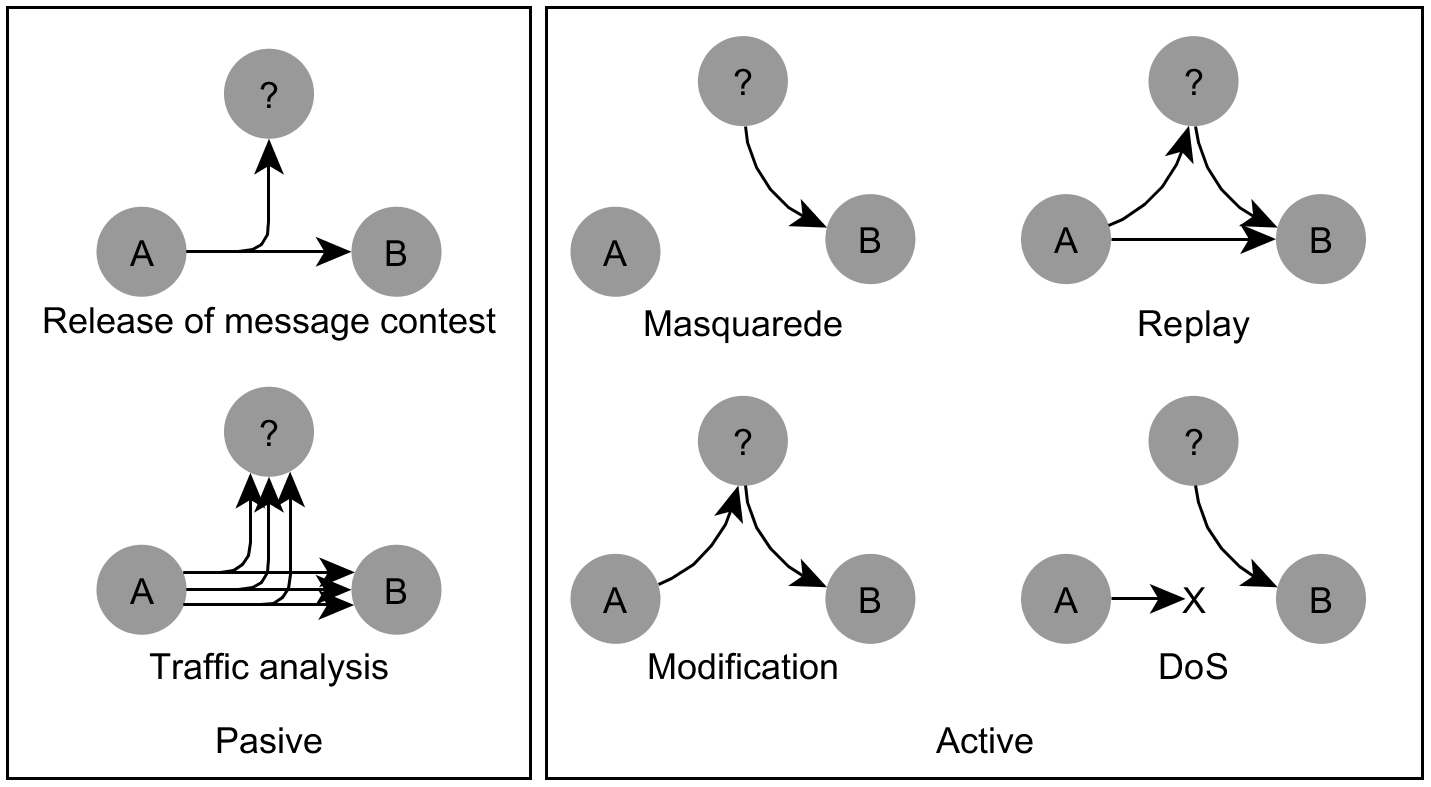
\includegraphics[scale=0.35]{a_attacks.png}
	\caption{Základné kategórie útokov. \cite{StallingsCryptographyandnetworksecurity}}
	\label{f:o_attacks}
\end{figure*}

\begin{figure*}[h]
	\centering
	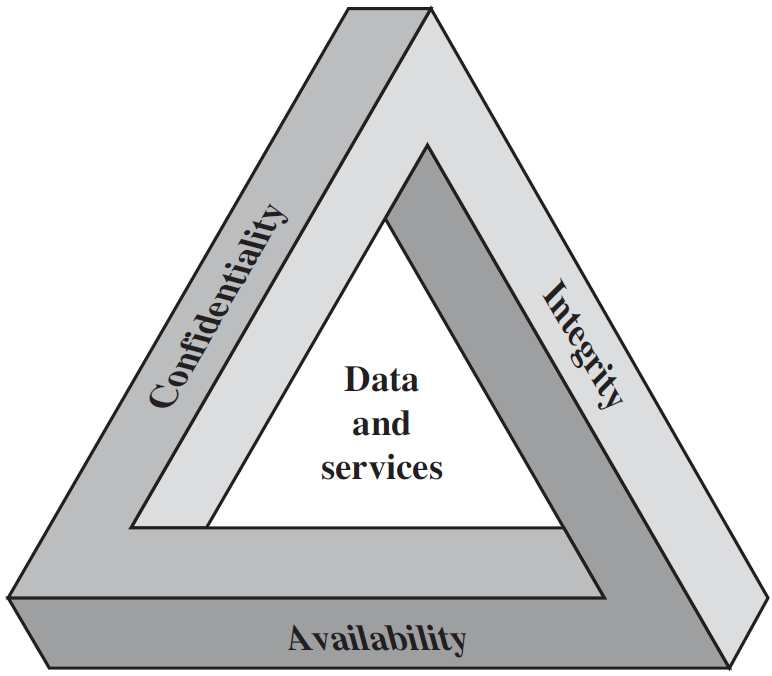
\includegraphics[scale=0.35]{a_CIA.png}
	\caption{Základné bezpečnostné ciele pre dáta a služby.\cite{StallingsCryptographyandnetworksecurity}}
	\label{f:o_cia}
\end{figure*}

%cite netowrk security
Keď vytvárame bezpečnú sieť, mali by sme brať do úvahy následovné\cite{bidgoli2006handbook}:
\singlespacing
\begin{itemize}
\item riadenie prístupu: autorizovaný používatelia majú možnosť komunikovať na príslušnej sieti, 
\item zabezpečiť dôvernosť: informácie na sieti ostanú utajené, 
\item zabezpečiť autentifikáciu: verifikovať, že používatelia sú tý, za ktorých sa vydávajú,
\item integritu: zabezpečiť, že správa nebola zmenená, modifikovaná alebo poškodená počas prenosu,
\item nepopierateľnosť: používateľ nemôže poprieť, že sieť použil.
\end{itemize}
\onehalfspacing

%Denial of service
%Unauthorized (accidental or intentional) disclosure
%Modification or destruction of information infrastructure components and data
%integrita
%nepopieratlenost
%autenticita
%confidentiality
%slassification
%DDOS
%

% Access – authorized users are provided the means to communicate to and from a particular network
% Confidentiality – Information in the network remains private
% Authentication – Ensure the users of the network are who they say they are
% Integrity – Ensure the message has not been modified in transit
%Non-repudiation - Ensure the user does not refute that he used the network

\subsection{Priebeh útoku} \label{s_attack}
Pre dostatočné zabezpečenie akéhokoľvek zariadenia alebo systému, je nutné rozumieť proti komu stojíte, chápať ich mentalitu, motiváciu, procesy a metódy, akými útočníci vyhľadávaju bezpečnostné slabiny ako ich zneužívajú a ako realizujú jednotlivé útoky. Týmito otázkami sa zaoberáme v kapitole.

Všeobecný a typický priebeh útoku na bezdrôtové komunikačné siete, ale aj na iné systémy je zobrazený na \ref{f:o_attack}. Zvyčajne sa skladá z nasledujúcich etáp \cite{bidgoli2006handbook}:

\singlespacing
\begin{itemize}
	\item Footprinting: získanie dostatočných informácií o cieľovom zariadení (TOE target of evaluation), veľkosti siete, počtu zariadení, infraštruktúre a získaní čo najviac relevantných informácií.
	\item Scanning: vyhľadávanie vhodných cieľov, vyhľadávanie bežiacich služieb a možných bezpečnostných slabín.
	\item Enumeration: podrobnejšie skúmanie vybraných zariadení a služieb.
	\item Získanie prístupu: zneužitie bezpečnostných slabín pre získanie prístupu k zariadeniu.
	\item Eskalácia privilégií: tento krok obnáša získanie dostatočných oprávnení na to, aby sme boli schopný získať úroveň prístupu potrebnú pre získanie citlivých dát a čo najvyšších oprávnení v systéme, keďže využitie slabín zvyčajne vedie k odkrytiu nových bezpečnostných slabín,
	\item Získanie citlivých dát: pozostáva zo získania prístupu a informácií o ďalších systémoch.
	\item Zahladenie stôp: spočíva v odstránení inkriminujúcich záznamov, operácií a opustenie systému, aby sme zanechali čo najmenej digitálnych stôp,
	\item Vytvorenie zadných vrátok: slúži pre možnosť jednoduchého opätovného navrátenia sa do napadnutého systému v budúcnosti,
	\item Odmietnutie služby: hovorí o vykonaní takých akcií, aby sme zamedzili prítup k zariadeniu alebo cieľovej služby ostatným používateľom a zariadení.
\end{itemize}

Existujú dva hlavné prístupy k riešeniu otázok zabezpečenia:
\singlespacing
\begin{itemize}
	\item Prevencia: správnym a vhodným spôsobom navrhnutá infraštruktúra, implementované bezpečnostné mechanizmy, smernice, správne a dostatočné fyzické zabezpečenie a podobné opatrenia,
	\item detekcia: cieľom detekcie je minimalizovať škody dôsledkom neošetrených hrozieb. Niektoré bezpečnostné situácie sa ošetriť nedajú, dajú sa iba detekovať. V takýchto prípadoch treba viesť evidenciu o vzniknutých situáciach pomocou auditných záznamov, logovaním kritických prístupov, vzniknutých chýb, môžu byť aj implementované metriky na zistenie neštandardného správania sa systému napr. dlhšia odozva zariadenia ako je normálne a im podobné.
\end{itemize}
\onehalfspacing

\begin{figure*}[h]
	\centering
	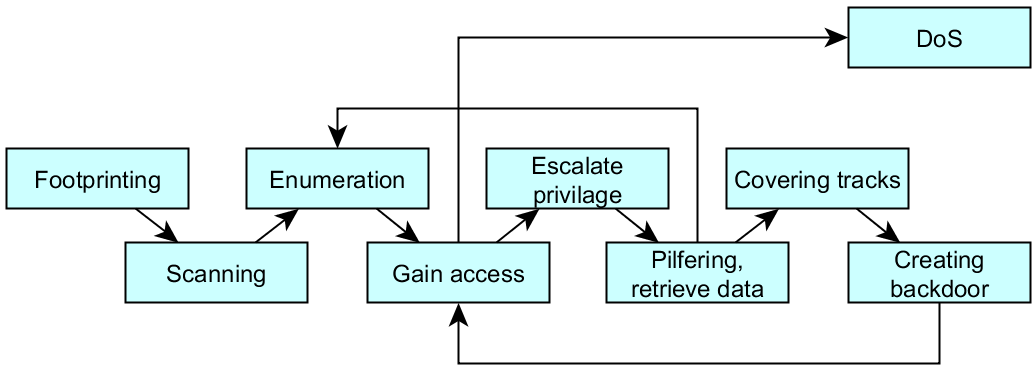
\includegraphics[scale=0.5]{a_attack.png}
	\caption{Všeobecný priebeh útoku.
	\cite{bidgoli2006handbook}}
	\label{f:o_attack}
\end{figure*}

\section{Kryptografia} \label{s_cryptography}
Základom kryptografie je umožňiť účastníkom komunikácie komunikovať po nezabezpečenom komunikačnom kanále tak, aby ostatné nezainteresované osoby neboli schopné získať obsah dôvernej komunikácie\cite{cryptodef}. Základné rozdelenie kryptografických prístupov je na obrázku \ref{f:o_kryptography}.

%handbook of applied kryptography
\begin{figure*}[!htb]
	\centering
	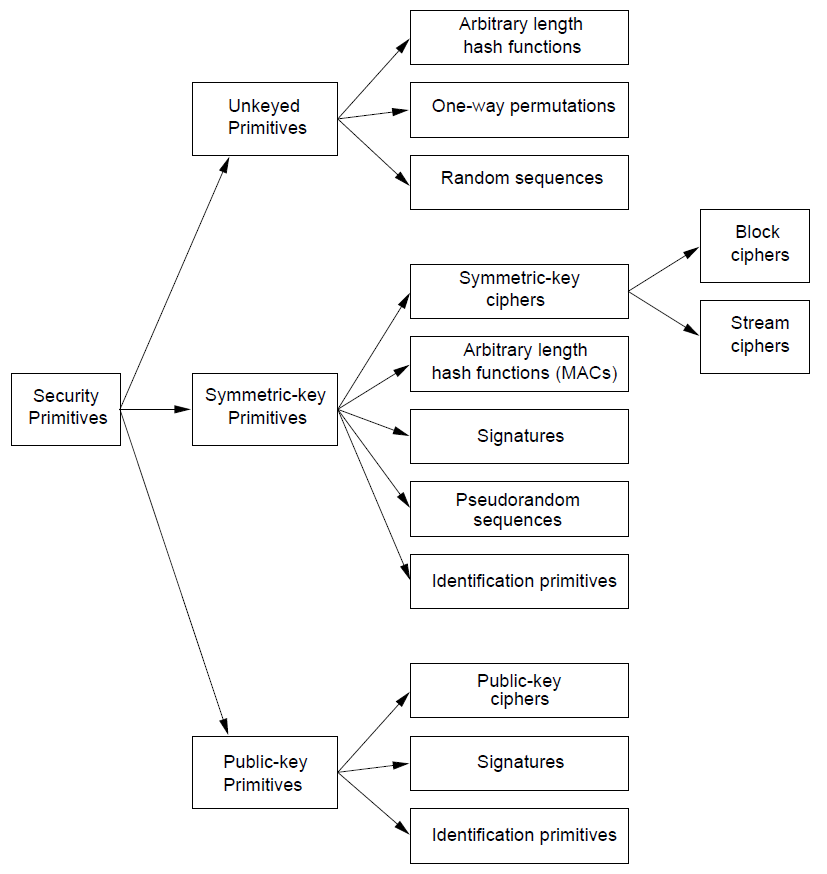
\includegraphics[scale=0.50]{a_kryptography.png}
	\caption{Rozdelenie kryptografických prístupov\cite{bidgoli2006handbook}.}
	\label{f:o_kryptography}
\end{figure*}

Základné rozdelenie kryptografických opatrení:
\singlespacing
\begin{itemize}
	\item Podľa typu použitých kľúčov:
		\subitem symetrické: na šifrovanie a dešifrovanie je použitý ten istý kľúč,
		\subitem asymetrické: na šifrovanie a dešifrovanie sú použité rôzne kľúče,
	\item podľa spôsobu transformácie nezašifrovaného textu na zašifrovaný text:
		\subitem substitučné šifry: nahrádzajú symboly z nezašifrovaného textu za nové,
		\subitem transpozičné metódy: poprehadzujú existujúce symboly medzi sebou na základe dopredu známych dohodnutých pravidiel,
	\item Podľa počtu spracovávaných dát:
		\subitem blokové: blokové šifrovacie algoritmy sú založené na šifrovaní dát po blokoch dopredu stanovenej pevnej dĺžky.
		\subitem prúdové: prudové šifrátory sú založené na šifrovaní dát prichádzajúcich do zariadenia bajt po bajtoch.
\end{itemize}
\onehalfspacing

%handbook of information and comunication security

Existujú štyri základné možnosti\footnote{Aj mnohé ďalšie napr. pod záštitou organizácie NIST: \url{http://csrc.nist.gov/groups/ST/toolkit/BCM/modes_development.html}} poprepájania kryptografických prvkov, ak potrebujeme poslať správu väčšiu ako je samotný kryptovaný blok, ktoré boli zavedené ako súčasť DES štandardu \cite{bidgoli2006handbook}:
\singlespacing
\begin{itemize}
	\item ECB: Electronic Codebook Mode,
	\item CBC: Cipher-Block Chaining,
	\item OFB: Output Feedback Mode,
	\item CFB: Cipher Feedback Mode.
\end{itemize}
\onehalfspacing

%elipticke a logaritmicke
%LUCIFER, DES, BLOWFISH, GOST, IDEA, RIJNDAEL

\subsection{Symetrické šifrovanie} \label{s_cpyt_symetric}
Princíp fungovania symetrických šifier je zobrazený na obrázku \ref{f:o_symetric}. Distribúcia kľúča použitého na šifrovanie prebieha zabezpečene napr. osobným stretnutím, alebo na základe vopred dohodnutých pravidiel.

\begin{figure*}[!hbt]
	\centering
	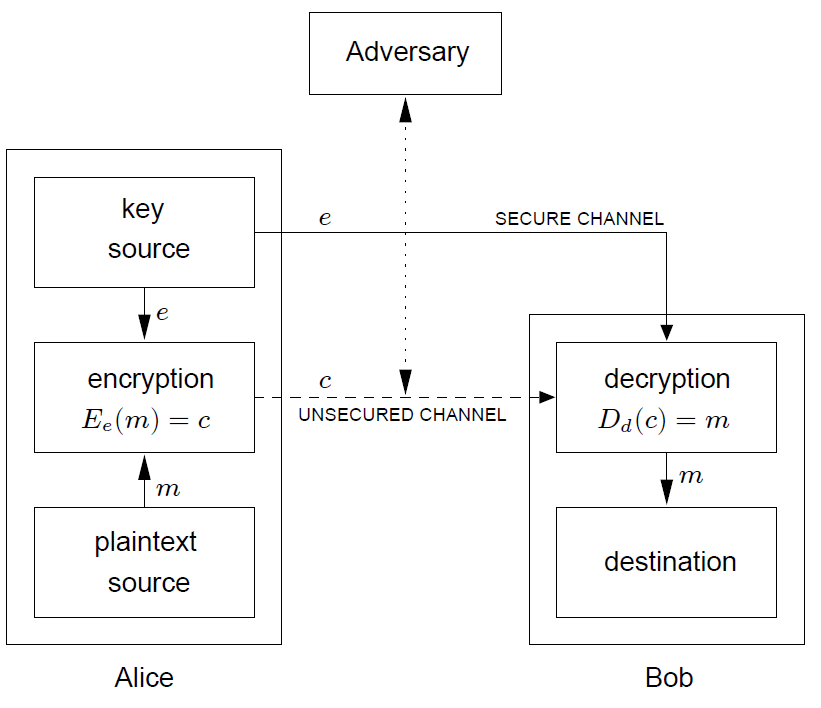
\includegraphics[scale=0.45]{a_symetric.png}
	\caption{Princíp fungovania symetrických šifier. \cite{cryptographyhandbook}}
	\label{f:o_symetric}
\end{figure*}

Komunikácia následne prebieha po bežnom nezabezpečenom kanále, ale šifrovane. Jediný nedostatok pri riešeniach problémov pomocou symetrických šifier je výmena kryptovacieho kľúča a komunikácia s viacerými používateľmi na naraz.

\subsubsection{AES} %DES,3DES,
Kryptovací štandard AES (Advanced Encryption System) vychádza z algoritmu s názvom Rijndael\footnote{\url{http://csrc.nist.gov/publications/fips/fips197/fips-197.pdf}}. Jedná sa o symetrickú blokovú šifru. Dĺžka spracovaváného bloku je pevne stanovený na 128 bitov, aj keď pôvodný navrhnutý algoritmus podporuje bloky s rôznou dĺžkou. Štandard dĺžky kľúčov 128, 192 a 256 bitov. Veľkosť vstupného a výstupného bloku je 128 bitov. Šifra sa zaraďuje medzi substitučno premutačné šifry.

Pre jednotlivé iterácie šifrovania sa z hlavného kľúča vygenerujú sub-kľúče, pomocou algoritmu key expansion, ktoré sú rôzne v iteráciach algoritmu.

Pre proces šifrovania je zadefinovaný pojem stav. Jedná sa o maticu o 4 riadkoch a 4 stĺpcoch a o veľkosti bunky 1 bajt. Nad touto maticou sa vykonáva celý proces šifrovania.

Operácie ščítania a multiplikácia sa vykonáva nad konečným poľom GF($2^8$).
%operácia násobenia a sčítania XOR Binárnymi ireducibilným polynómom rádu menším ako 8
Výhoda AES štandardu je v jeho rýchlosti, ľahkej hardvérovej  implementovateľnosti. Zložitosť AES spočíva v nelineárnej operácií SubBytes a v permutáciach realizovaných rotáciou riadkov a transformáciou stĺpcov.

Proces šifrovania nad aktuálnym stavom spočíva v 4 operáciach:

\begin{itemize}
	\item \textbf{AddRoundKey}: k aktuálnemu stavu sa pripočíta, priXOR-uje, aktuálna hodnota vygenerovaného pod-kľúča \ref{f:a_AES_round},
	\item \textbf{SubBytes}: realizuje nelineárnu transformáciu, ktorá nahradí každú hodnotu zo stavu inou hodnotou z inicializovanej lookup tabuľky,
	\item \textbf{ShiftRows}: realizuje posun riadku doľava po bajtoch, na základe indexu riadku, ktorý začína od nuly \ref{f:a_AES_shift},
	\item \textbf{MixColumns}: transformácia sa aplikuje na celý stĺpec aktuálneho stavu\ref{f:a_AES_columns}.
\end{itemize}

%ax^-1+c

\begin{figure*}[!htb]
	\centering
	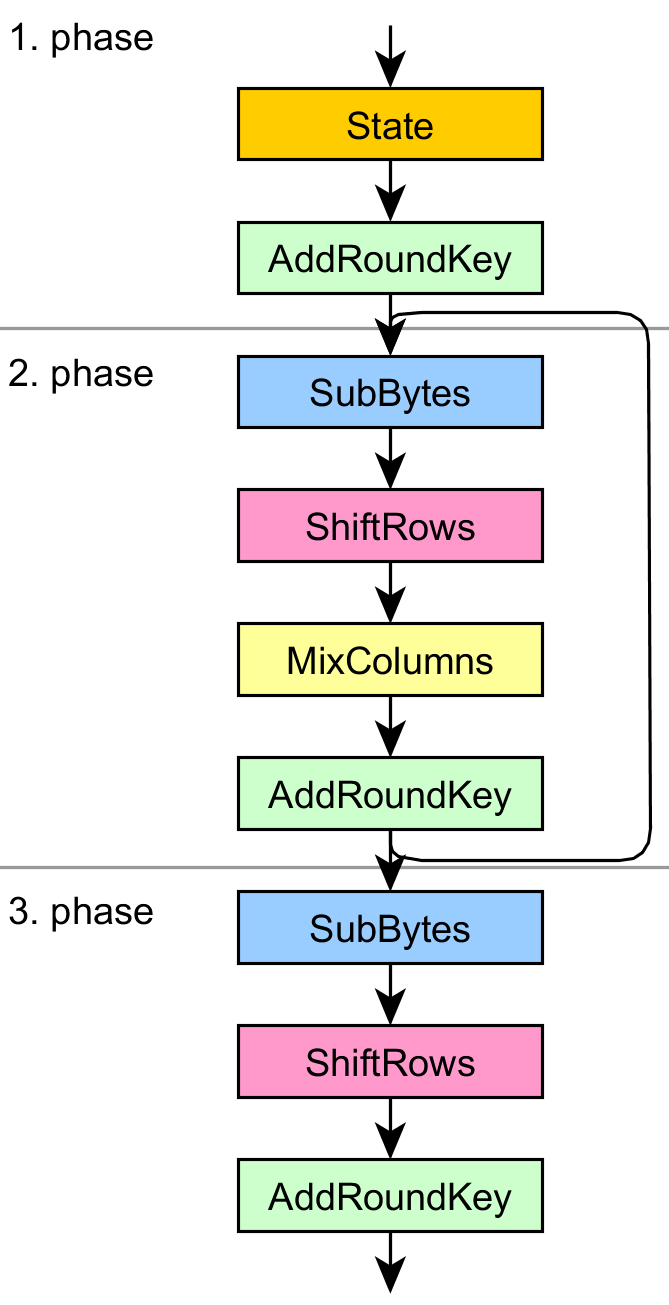
\includegraphics[scale=0.2]{c_AES_alg.png}
	\caption{Algoritmus štandardu AES\cite{AESAnimation}.}
	\label{f:a_AES_animation}
\end{figure*}

\begin{figure*}[!htb]
	\centering
	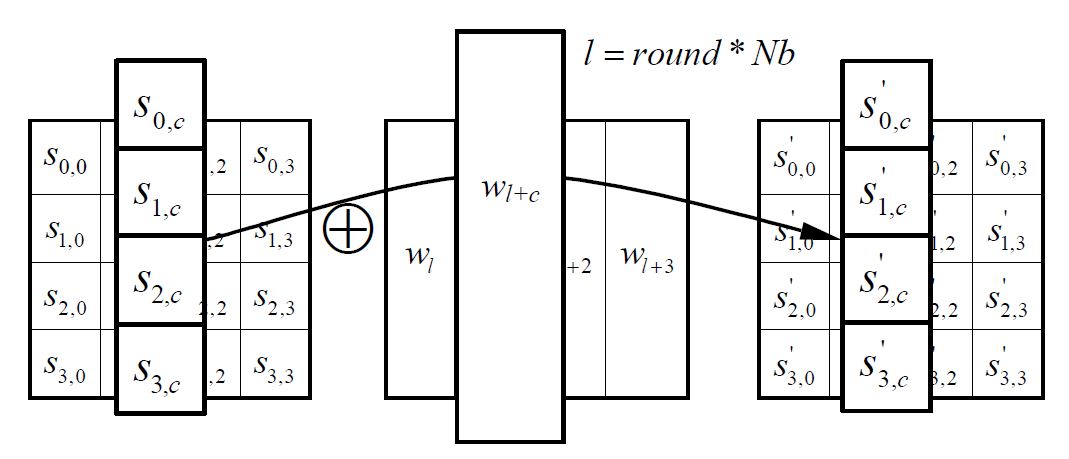
\includegraphics[scale=0.2]{c_aes_roundkey.png}
	\caption{AddRoundKey\cite{AES}.}
	\label{f:a_AES_round}
\end{figure*}

\begin{figure*}[!htb]
	\centering
	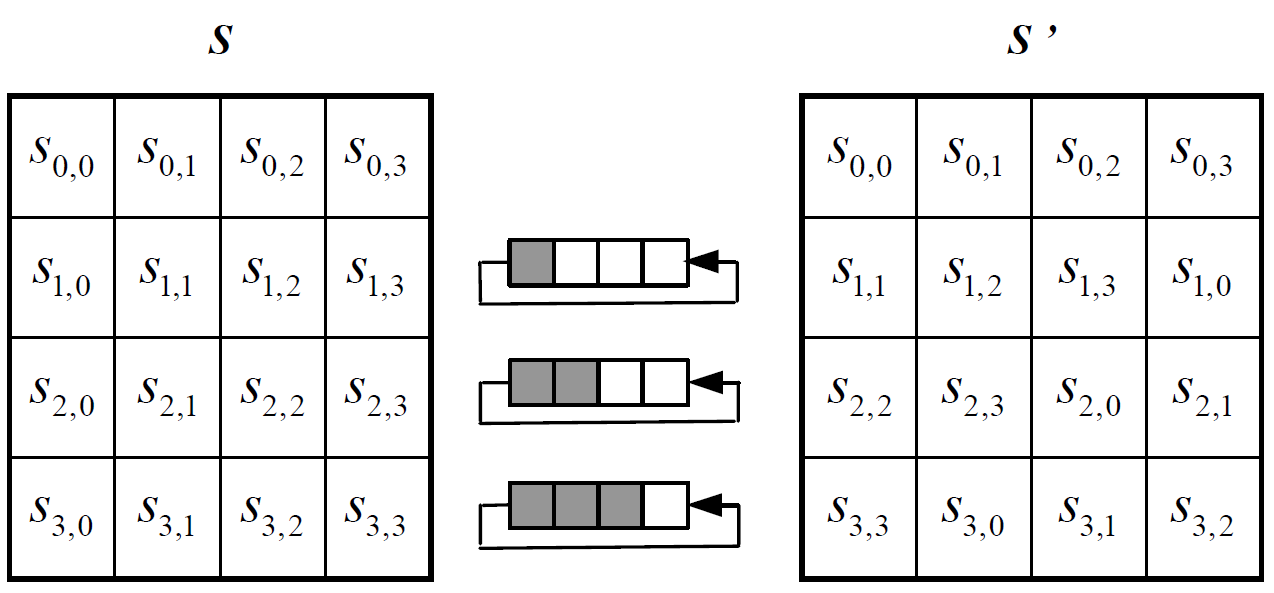
\includegraphics[scale=0.165]{c_aes_ShiftRows.png}
	\caption{Operácia shift rows\cite{AES}.}
	\label{f:a_AES_shift}
\end{figure*}

\begin{figure*}[!htb]
	\centering
	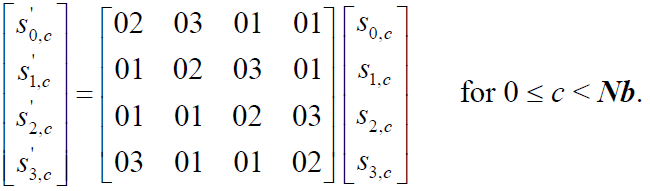
\includegraphics[scale=0.35]{c_aes_collumns.png}
	\caption{MixColumns\cite{AES}.}
	\label{f:a_AES_columns}
\end{figure*}

\begin{table}
	\centering
	\caption{Odporúčaný počet kôl šifrovania v závislosti od dĺžky kľúča\cite{AES}.} 
	\label{table:AES_pocet_iteracii}
	\begin{tabular}{|c|c|c|c|}
		\hline
		 & \textbf{dĺžka kľúča} [bit] & \textbf{veľkosť šifrovaného bloku} & \textbf{počet iterácií} \\
		\hline
		AES-128 & 4 & 4 & 10\\
		\hline
		AES-192 & 6 & 4 & 12\\
		\hline
		AES-256 & 8 & 4 & 14\\
		\hline
	\end{tabular}
\end{table}

%\subsubsection{3DES} %PGP %KEY %IDEA %blowfist twofisch %Asymetrické šifry: Ruksakový systém, McElieceov, RSA, Rabinov, systémy na

\subsection{Asymetrické šifrovanie}  \label{s_cpyt_asymetric}
Na rozdiel od symetrického šifrovania, pri asymetrickom šifrovaní existuje pár kľúčov, ktoré sú navzájom na sebe závislé. Tieto kľúče sa nazývajú privátny a verejný. Komunikácia prebieha iba po nezabezpečených komunikačných kanáloch. Používateľ, ktorý zašifroval správu niekoho verejným kľúčom, už ju nevie dešifrovať. Dešifrovať správu vie iba osoba, ktorá vlastní privátny kľúč a pre ktorú je správa určená.  sú označované aj názvom PKI.

Problém, ktorý vzniká pri asymetrickej kryptografií je, že ako odosielateľ si nemusíme byť istý, že osoba s ktorou komunikujeme je tá, za ktorú sa vydáva. Od toho vznikajú služby tretích strán s názvom certifikačné autority.

\begin{figure*}[!htb]
	\centering
	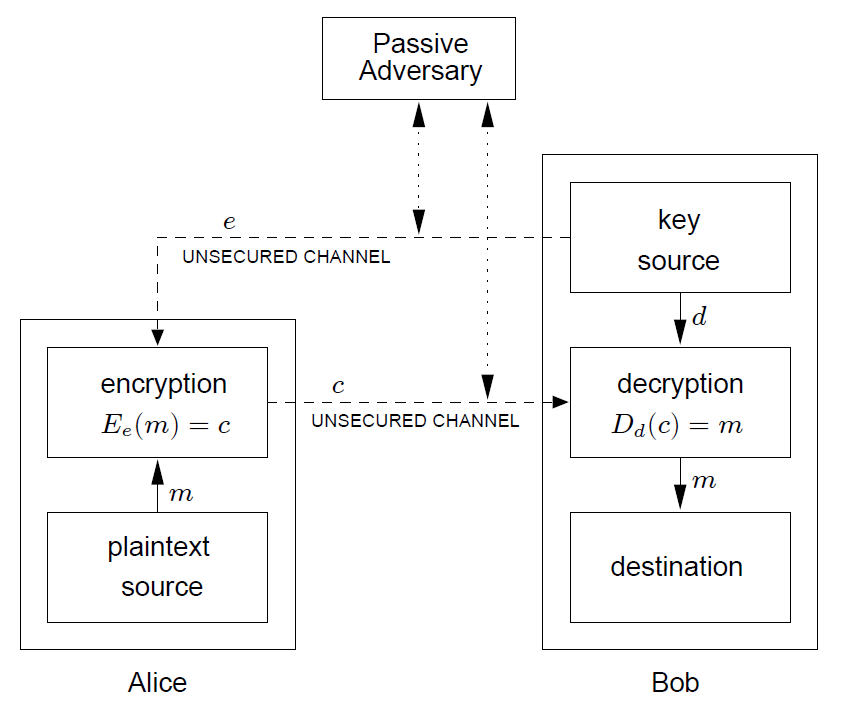
\includegraphics[scale=0.5]{a_asymetric.png}
	\caption{Princíp fungovania asymetrických šifier. \cite{cryptographyhandbook}}
	\label{f:o_asymetric}
\end{figure*}

%báze EC. Podpisové schémy. Autentizácia dokument
\subsubsection{RSA}
RSA algoritmus sa zaraďuje do asymetrickej kryptografie. Princíp fungovania je založený na probléme faktorizácie, rozkladu modulu na činitele, násobku dvoch veľkých prvočísiel. Udávaná zložitosť algoritmu je $O(N^3)$ \cite{rsalesson}.

Princíp inicializácie a fungovania kryptosystému RSA je nasledovný. Vygenerujú sa dve rôzne prvočísla označené $p$ a $q$. Následne sa vypočíta modul $n$, vynásobením vygenerovaných prvočísel $p$ a $q$: $n= p \times q $ \cite{rsalesson}.
%fi kolko cisiel mensich ako n je nesudelitencyh s n
Výpočet Eulerovej funkcie $\varphi(n)$ je jednoduchý, keďže modul je tvorený z dvoch prvočísiel: $\varphi(n)=(p-1)\times(q-1)$. Následne sa zvolí parameter $e$, tak aby spĺňal podmienku $1<e<\varphi(n)$ a $gcd(\varphi(n),e)=1$. Druhý parameter $d$ sa dopočíta zo vzorca $ed=1 mod \varphi(n)$ \cite{rsalesson}.

Verejný kľúč je tvorený dvojicou [n, e] a privátny kľúč je tvorený dvojicou [n, d].
Proces šifrovania a dešifrovania je nasledovný. Otvorený text, označený $x$, šifrujeme pomocou $E(x)=x^e mod n$. Šifrovaný text, označený $y$, dešifrujeme obdobne pomocou nasledovného vzorca $D(y)=y^d mod n$ \cite{rsalesson}.

%zavislosti a ed e je mensi p a q by mali byt co najdelej od seba

%\subsection{Alternativne pristupy}  \label{s_alternatives}
\subsubsection{ECC: Elliptic curve cryptography}
Kryptografický systém založený na ECC stavia na výpočtovej zložitosti problému diskrétneho logaritmu DLP.
%Elliptic Curve Discrete Logarithm Problem

%\clearpage

Typicky sa pre eliptické krivky používa rovnica nasledovného tvaru $E:y^2=x^3+ax+b$. Je to parametrizovaná rovnica parametrami $a$ a $b$. Zo vzorca vyplýva, že výsledný graf je symetrický okolo osy x.
Odporúčané parametre krivky sú také, ktoré spĺňajú podmienku: $4a^3 + 27b^2\neq0  mod(p)$. Tá garantuje, že rovnica má práve jedno riešenie v reálnej rovine.

\begin{figure}[h]
	\centering
	\adjustbox{angle=-90}%
	{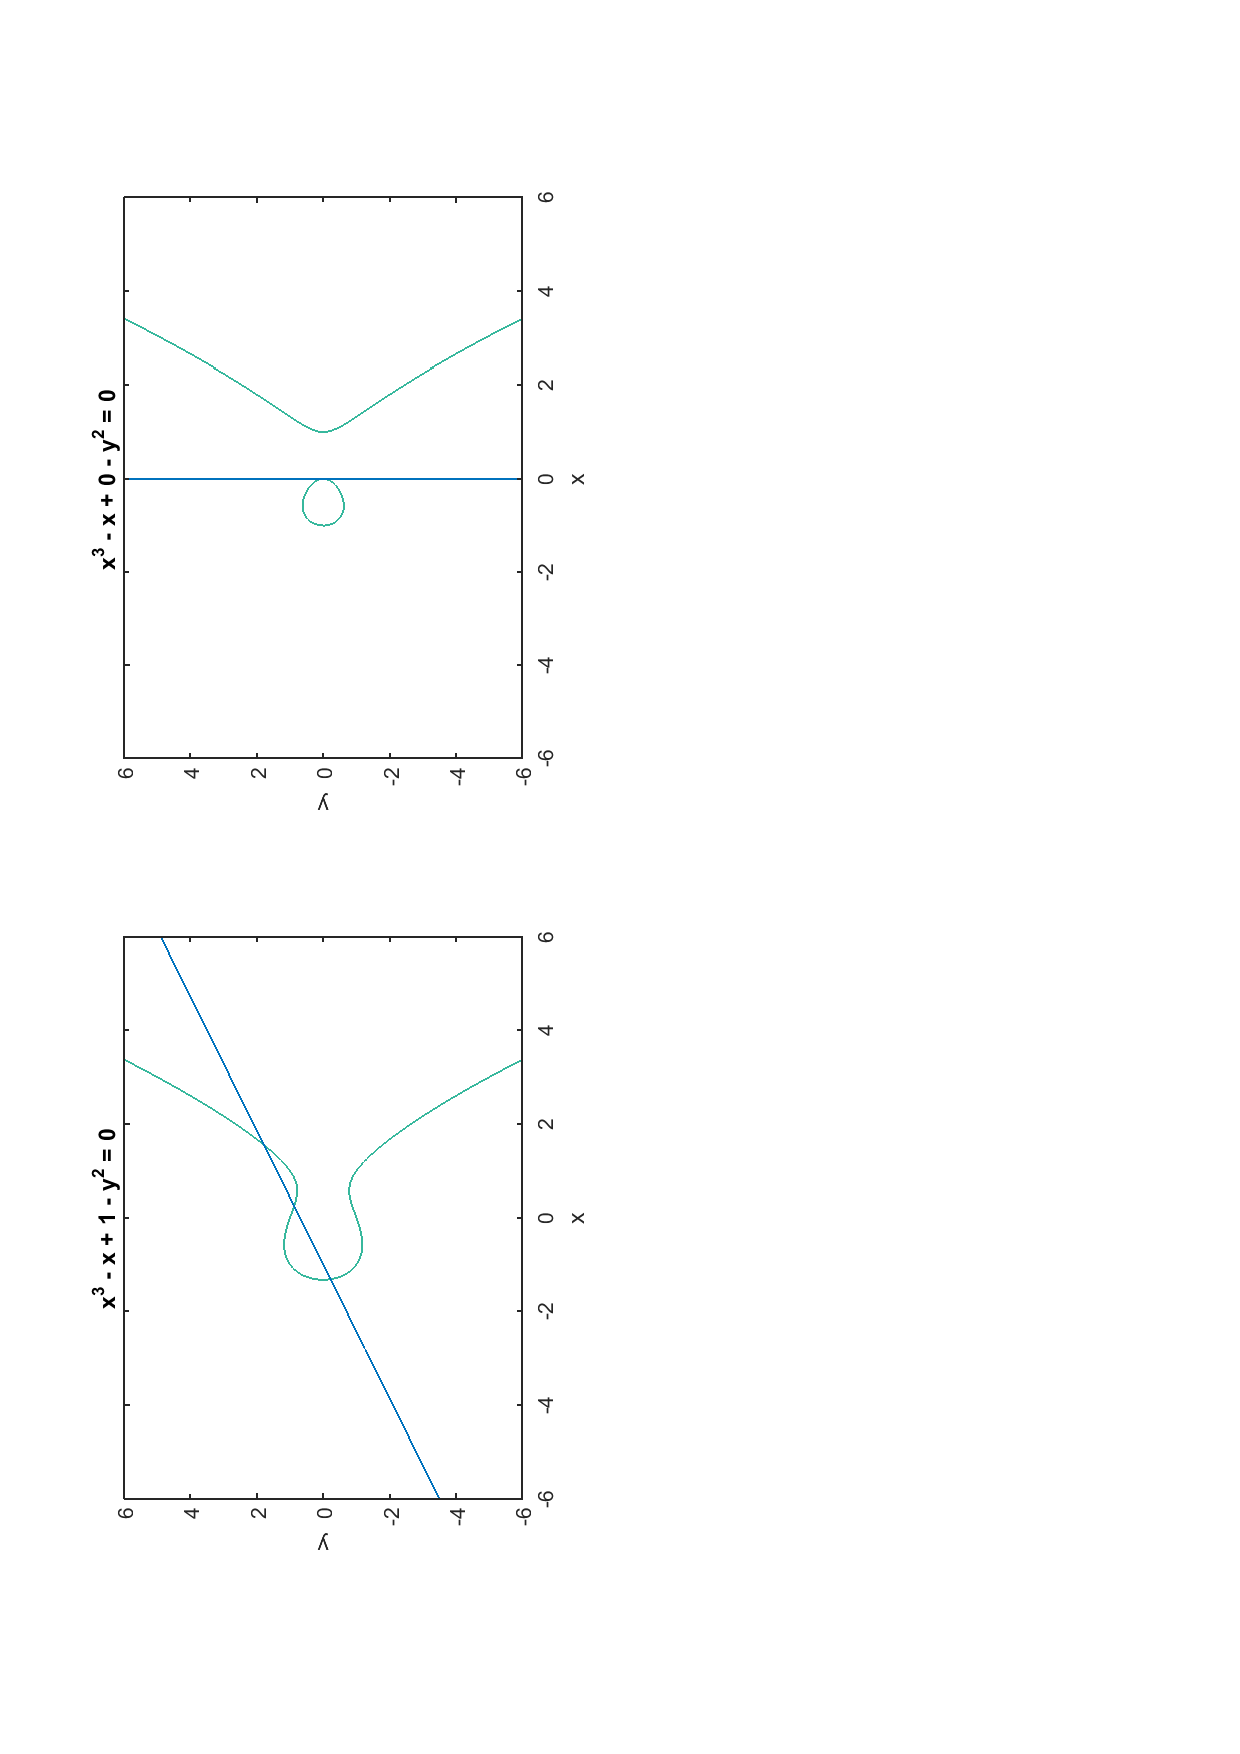
\includegraphics[scale=0.6, trim={0cm 1cm 10cm 0cm}, clip ]{ECC.pdf}}
	\caption{Príklady eliptických kriviek s rôznymi parametrami $a$ a $b$.}
	\label{f:o_ECC}
\end{figure}

%discretny logaritmus DL O(N^3)
Výpočty prebiehajú nad konečným, ale dostatočne veľkým poľom definovaným parametrom $p$: $E:y^2=x^3+ax+b mod(p)$.
Odporúčanie pre parameter $p$ je, aby to bolo prvočíslo a spĺňalo podmienku $p mod(3) = 4$.

Doménové parametre sú definované šesticou (p, a, b, G, h, n). Jedná sa o parametre krivky $a$ a $b$, použitý generátor grupy $G$, prvočíslo p, ktoré určuje veľkosť konečného poľa nad ktorým sa vykonávajú výpočty, rád grupy $h$ a kofaktor $n$\cite{ecclesson}.

Pre zabezpečenie adekvátnej bezpečnosti sa odporúča používať overené generátory pre danú eliptickú krivku.

Pre prácu nad množinou bodov patriacich krivke, boli zadefinované operácie ščítania a násobenia dvoch bodov. Každý z bodov sa skladá z  koordinátov x a y. Pre úplnosť a správnosť operácií bol dodefinovaný bod v nekonečne, pre ktorý platí: $P+O=O$ a $O=-O$.
Pre inverzný bod P(x,y) platí -P=(x,-y).

Operácia ščítania je priamka vedená cez body krivky P a Q a  pretne krivku v bode -R: P+Q=-R. Aby sme dostali výsledok R, je potrebné spraviť inverziu vypočítaného bodu -R. Verí sa, že operácia sčítania je dostatočne dobrá jednosmerná funkcia (tzv. trapdoor).

Výpočet ščítania dvoch bodov P a Q sa implementuje jednoducho, na základe analytickej geometrie a vzorcov pre strmosť priamky.
%(y=kx+y)%
Ak sa ščítavajú dva rôzne body, výpočet prebieha pomocou vzorca: $\alpha = \dfrac{ y_{Q}-x_{P}}{x_{Q}-x_{P}}$. Ak sa jedná o dotyčnicu krivky výpočet $\alpha$ je nasledovný: $\alpha = \dfrac{3x_{P}^2 + a}{2y_{P}}$. Súradnice x a y výsledného bodu sa vypočítajú
$x_{R}$ = $\alpha ^2 - x_{P} - x_{Q}$ a 
$y_{R}$ = $\alpha (x_{R} - x_{P}) + y_{P}$ \cite{ecclesson}.

Multiplikácia bodu P k-krát: $k\times P$ nieje nič iné, ako k-krát vykonané sčítanie bodu P $P+P+...P$ a označuje sa aj ako point doubling. $2\times P = P+P$\cite{ecclesson}.

Pri dostatočne veľkom konečnom poli (parameter p), nie sme schopný v reálnom čase zistiť, koľko-krát sme vykonali operáciu point doubling z počiatočného bodu generátora grupy pri privátnom kľúči k.

Je dokázené, že akákoľvek priamka ktorá pretína graf krivky, pretne graf práve v troch bodoch. Ak priamka krivku nepretne, definuje sa výsledný bod v nekonečne $O$.

Pre prácu s PKI infraštruktúrou bol zadefinovaný privátny kľúč, ktorý je tvorený práve jedným parametrom $k$, ktorý určuje, koľko-krát sme vykonali operáciu point doubling nad generátorom cyklyckej grupy. Privátny kľúč by mal spĺňať podmienku $1<k<n-1$. Verejný kľúč pre eliptickej kryptografií je tvorený doménovým parametrom a výsledným bodom $C$ po vykonaní operácií point doubling $C=kG$.

Pri generovaní certifikátu certifikačnou autoritou, je subjekt nútený dokázať, že je naozaj vlastníkom daného privátneho kľúča $k$, aby mu mohol byť vystavený certifikát\cite{ecclesson}.

Tak isto existuje aj spôsob, ako si vymeniť kľúč, bez toho, aby sme ho mali dopredu dohodnutý. Jedná sa o modifikáciu výmeny kľúča pomocou metódy DH (Diffie Hellman) označovaného ako ECDH. Na podpisovanie dokumentov pomocou ECC sa používa algoritmus označovaný ako ECDSA. Ako aj RSA, tak aj pri ECC fungujú certifikačné autority, ktoré garantujú, že daný subjekt vlastní príslušný verejný kľúč\cite{ecclesson}.

Veľkou výhodou eliptických kriviek, oproti algoritmu RSA je v tom, že poskytujú rovnakú bezpečnosť, pri oveľa menšej dĺžke použitého kľúča. To znižuje nároky aj prenosové pásmo a veľkosť vymieňaných správ. Samotný algoritmus je jednoduchší na implementáciu ale potrebuje dostatočne dobrý generátor náhodných čísiel. Porovnanie bezpečnosti pri rovnakej dĺžke kľúča je v tabuľke \ref{table:PorovnanieDlzkyKlucov}. 

%defaulte elgamal je nahodny cize rovnaka sprava sa zakryptuje rovnako, na rozdiel od RSA, ak sai tam nedame jeden byte nahodne cislo.

\begin{table}
	\centering
	\caption{Porovnanie dĺžky kľúčov\cite{ecclesson}.} 
	\label{table:PorovnanieDlzkyKlucov}
	\begin{tabular}{|l|l|l|}
		\hline
		\textbf{ECC} [bit] & \textbf{RSA a DH} [bit] & \textbf{Symetrické šifry} \\
		\hline
				\hline
		160 & 1024 & 80 \\
		\hline
		224 & 2048 & 112 \\
		\hline
		256 & 3072 & 128 \\
		\hline
		384 & 7680 & 192 \\
		\hline
		512 & 15360 & 256 \\
		\hline
	\end{tabular}
\end{table}

%\subsubsection{logaritmic}

\subsection{Porovnanie HW a SW kryptografických implementácií} \label{s_cpyt_comparison}
Nasledujúca podkapitola sa snaží čitateľovi poskytnúť porovnanie hardvérových a softvérových riešení v podobe ich silných a slabých stránok. \\
\textbf{Softvérové riešenia:}
	\begin{itemize}
		\item \textbf{Výhody softvérových riešení sú predovšetkým:}
		\begin{itemize}
			\item v rýchlom prototypovaní,
			\item jednoduchej aktualizácií systému na novšiu verziu,
			\item používajú prístupy v programovaní, ktoré sú človeku prirodzene bližšie ako: OOP, XML, JSON,
			\item jedna iterácia vývoja, vykonanie nových zmien a nasadenie softvéru je oveľa rýchlejšie ako pri návrhu hardvéru,
			\item nízka cena na nasadenie služieb a opravu chýb.
		\end{itemize}
		\item \textbf{Nevýhody:}
		\begin{itemize}
			%\subsubitem náchylné na programátorské chyby,
			\item vznikajú problémy, kde a ako uložíme citlivé heslá,
			%, zdieľané tajomstvá hash so soľou,
			%\subsubitem brute-force,
			%\subsubitem slabín systému,
			\item nedostatočné zabezpečenie, pri ktorom dochádza pri zlom ošetrení používateľských vstupov: XSS, CGI, 
			\item neošetrenie alebo nesprávne ošetrenie používateľského vstupu zvyčajne vedie k možnému code insertion, injection, shellcode,
			\item systémy sú náchylné na modifikácie neplatných cache záznamov,
			\item nepremazanie dynamických pamätí typu RAM pri preplánovaní procesu a jej následné pridelenie inému procesu dokáže sprístupniť citlivé dáta novému procesu,
			\item dajú sa použiť segmentation chyby k prístupu k neautorizovaným dátam,
			\item zneužívanie pretečení zásobníkov a buffrov,
			\item odchytenie nového firmvéru alebo updatov môže viesť k odhaleniu bezpečnostných slabín, alebo k získaniu hard-coded prihlasovacých údajov,
			\item bezpečnosť celého systému často závisí na bezpečnosti celého operačného systému, vzdelanosti používateľa pri útokoch typu social engineering, od bežiacich služieb a od spustených používateľských programov, ktoré môžu kompromitovať ostatné bežiace služby, procesy alebo zabezpečenia, od nastavení systému a jeho konfigurácie,
			\item niektoré nedostatočné bezpečnostné opatrenia sa dajú ľahko obísť,
			\item zneužitím jednej bezpečnostnej slabiny sa môžu postupne odkrývať ďalšie,
			\item kvôli získaniu citlivých dát z dynamických RAM pamätí sú útočníci schopný pamäť ochladiť tekutým dusíkom, extrahovať ju z pôvodného systému do nového a na novom systéme robiť následnú analýzu a zber citlivých dát,
			\item kódy sú náchylné na reverzné inžinierstvo, disassembly a dekompiláciu. Často následne dochádza aj k modifikácií kódu aj počas vykonávania. Existujú však aj isté opatrenia v podobe code obfuscation, ochrany proti dekompilácií, odstraňovaním nadbytočných symbolických informácií alebo pomocou zabudovanej kontroly toku programu.
			%DES butoforce
		\end{itemize}
	\end{itemize}
	
	\textbf{Hardvérové riešenia:}
	\begin{itemize}
		\item \textbf{Výhody:}
		\begin{itemize}
			\item sú ideálne na ukladanie klúčov, ktoré niesú natvrdo vložené do firmvéru, ale sú bezpečne uložené v špecializovaných registroch a pri nutnej aktualizácií firmvéru sa tieto informácie neprenášajú spolu s novou binárkou,
			\item zvyčajne poskytujú pridanú hodnotu v podobe overených bezpečnostných služieb, programátori ich nemusia nanovo implementovať softvérovo, 
			\item nižšia prúdová spotreba,
			\item vyšší výpočtový výkon ako pri rovnocenných softvérových implementáciach,
			\item riešenia sú dedikované a odlaďované na vykonávanie špecifickej funkcie,
			\item implementované hardvérové ošetrenia proti čítaniu naprogramovaného firmvéru,
			\item presne daná nemeniaca sa funkcia, ktorá ma prístupné zvonku iba zabezpečené rozhrania,
			\item dedikovaný hardvér ktorý rieši iba to čo má, často implementuje dodatočné bezpečnostné mechanizmy proti rôznym typom útokom napr. generovanie náhodných hodnôt na nepoužívaných zberniciach alebo vykonávanie nadbytočných náhodných inštrukcií,
%			\item IP jadrá, zvyšujú bezpečnosť a chránia výrobcu,
			
			\item na hardvérové systémy sa ťažšie aplikuje revezné inžinierstvo, využívajú sa špecializované a alternatívne prístupy napr. pomocou elektronových mikroskopov, röntgenov, presné odfrézovanie vonkajšieho obalu a analýza čipu po jednotlivých vrstvách na samotnom kremíku. Podobne sa dá realizovať aj analýza naprogramovaných ROM pamätí,
			\item útoky sú všeobecne náročnejšie na realizáciu. Realizujú sa útoky na časovanie, generujú sa krátke nábežné hrany, neštandardné napäťové úrovne hodinového signálu mimo prevádzkových parametrov,  
			\item realizujú sa útoky, kde sa monitorujú zmeny, poklesy a výkyvy na napájaní, tzv. side channel monitoring,
			\item monitorujú sa zmeny v elektromagnetickom vyžarovaní samotného čipu,
			\item často sú implementované hardvérové detekcie manipulácie so zariadeniami (temper proof alebo temper detection) napr. POS terminály pri fyzickom otvorení vymažú internú dynamickú pamäť.			

			%odolne ore falsovanie, implementovane hw osetrenia proti utokom, zmazu sa alebo 

		\end{itemize}
		\item \textbf{Nevýhody:}
		\begin{itemize}
			\item zvyčajne ťažšie odlaďovanie požadovanej funkcionality. Postupne však dochádza k vylepšovanie simulačných systémov napr. ModelSim,
			\item sú potrebné rozsiahlejšie znalosti na správny návrh a odladenie systému. Správne a vhodné rozmiestnenie súčiastok, potrebné znalosti z rôznych oblastí od problematiky vysokofrekvenčných signálov, šírenie signálov na dlhom vedení, správne impedančné prispôsobenie vstupov a výstupov, elektrotechniky, limity použitých technológií, teplotné zavislosti až po distribúciu tepla,
			\item rozšírenie systému o novú funkcionalitu vyžaduje väčšie množstvo vynaložených nákladov a času,
			\item čas na nasadenie produktu je n-násobne dlhší ako pri softvérových riešeniach,
			\item návrh trvá niekoľko iterácií, kým sa systém správne odladí. Väčšia dostupnosť a znižujúca sa cena FPGA čipov a ASIC (Application Specific Integrated Circuit) na druhú stranu podstatne urýchľuje prvotný návrh a odladenie,
			\item výskyt špecifických chýb sa často odhalí až pri reálnej prevádzke, alebo až po istom čase,
			\item následná ťažšia celková systémová údržba a opravy,
			\item riešenia pre kritické operácie v podobe bezpečného návrhu, verifikácie a systémy odolné voči poruchám realizované pomocou informačných, hardvérových alebo časových redundancií sú drahšie v podobe vynaložených prostriedkov,
			\item pokiaľ je dedikovaný hardvér oddelený od odstatných komponentov systému a nieje všetko vnorené na jednom čipe, pri komunikácií s hardvérovým zariadením môže prísť k odchyteniu nešifrovaných dát alebo komunikácie pri nedostatočnom fyzickom zabezpečení zariadenia alebo objektu.
			
			%Ak má niekto prostredky tak ho nezastavíte, môžte ho len spomaliť. často navyše špecializované zariadenia a tým sa predražuje a predlžuje aj čas potrebný
		\end{itemize}
	\end{itemize}


\section{Bezdrôtové komunikačné protokoly} \label{s_protocols}
%UDP bez potvrdzovania
%TCP s potvrdzovanim
\subsection{WPAN siete}
Štandardizáciou a vývojom protokolov v oblasti LAN/MAN sietí sa stará organizácia s označením IEEE
802 \footnote{\url{http://grouper.ieee.org/groups/802/15/pub/Download.html}}. V štandardoch definuje odporúčané postupy pre jednotlivé vyvíjané a udržiavané typy sietí. V
inteligentných domácnostiach sa najčastejšie zvyknú používať siete s označením 802.15 WPAN (Wireless Personal Area Network).
\subsection{IEEE 802.11}
Prvý spomenutý štandard nepatrí do sietí typu PAN ale WLAN. Stojí za spomenutie aj keď cena, spotreba a nároky na hardvér a softvér sú pomerne vysoké. Disponuje ale veľkými prenosovými rýchlosťami v závislosti od štandardu a ponúka aj dostatočné zabezpečenie v podobe WPA2. Maximálna vzdialenosť medzi uzlami je 100m. 
\subsection{IEEE 802.15.1}
Prvý štandard z rodiny sietí WPAN je známy pod označením Bluetooth
\footnote{\url{https://www.inf.ethz.ch/personal/hvogt/proj/btmp3/Datasheets/Bluetooth_11_Specifications_Book.pdf}}. Za pár rokov existencie bolo vydaných pár verzií štandardu, ktoré sú postupne vylepšované a prispôsobované požiadavkám trhu.
Bluetooth 2 označovaný aj BR/EDR (Basic Rate/Enhanced Data Rate) podporuje v štandardnú rýchlosť 1 Mbps a v rozšírenej verzii rýchlosť až 2 Mbps.
Bluetooth 3 HS (High Speed) je určený hlavne pre streamovanie audia s prenosovou rýchlosťou do 24 Mbps.
Bluetooth 4 je označovaný aj ako LE (Low Energy). Disponuje kryptovaním 128-bit AES a bol vytvorený tak aby mal malú spotrebu energie. Najnovšia verzia jadra 4.2 \footnote{\url{https://www.bluetooth.com/specifications/adopted-specifications}} umožnuje komunikovať zariadeniam cez bránu s internetom a podporuje adresovanie IPv6 označované ako 6LoWPAN.
%\footnote{\url{https://www.bluetooth.org/DocMan/handlers/DownloadDoc.ashx?doc_id=286439&_ga=1.129180943.2007277090.1462873055}}
Dosah Bluetooth zariadení je udávaný vo výkonových triedach Class 1-0.1W, Class 2-2.5 mW a Class 3-1 mW.
\subsubsection{Bluetooth}

\subsubsection{Bluetooth SMART, BLE}

\subsection{IEEE 802.15.3}
V štandarde 802.15.3 boli zadefinované požiadavky na fyzickú vrstvu a vrstvu MAC (Media Access Control) tak aby bolo možné prenášať dáta väčšou rýchlosťou. Tieto siete sa označujú HR-WPAN (High Rate).

\subsection{IEEE 802.15.4}
Štandardy pod týmto identifikátorom sú označované ako LR-WPAN (Low Rate). Nad týmto štandardom sú postavené protokoly známe pod názvom Zigbee, Z-Wave alebo Thread.
Podporované topológie siete pri ZigBee sú mash a star. Zariadenia implementujúce štandard Zigbee sa vyznačujú nízkou cenou a malou spotrebou. Maximálny počet uzlov v sieti vyplýva zo smerovacej hlavičky na sieťovej vrstve, ktorá má dĺžku 16 bitov. Nevýhodou štandardu sú pomerne malé prenosové rýchlosti, nie je vhodné na streamovacie účely, ale na prenos malých objemov dát. Má zabudované kryptovanie typu AES s dĺžkou 128 bitov. Dosah ZigBee uzla je variabilný od použitého vysielacieho výkonu pri platformách XBee sa vysielací výkon pohybuje v rozmedzí od 1 mW až po 1 W.
\footnote{\url{http://www.ni.com/white-paper/4450/en/}}
Módy Zigbee uzlov:
%\singlespacing
\begin{itemize}
	\item AT (Attention mód) - Command mód: slúži na priamu komunikáciu so ZigBee uzlom, používa sa na jeho konfiguráciu,
	\item transparent mód: slúži na posielanie dát cez sieť.
\end{itemize}
\onehalfspacing

Typy uzlov v ZigBee sieti:
\singlespacing
\begin{itemize}
	\item Fully functional device:
		\subitem koordinátor: v sieti musí byť aspoň jeden,
		\subitem router: je zodpovedný za smerovanie paketov,
		\subitem end device: koncové zariadenie.
	\item reduced function device:
		\subitem end device.
\end{itemize}
\onehalfspacing

%black hat 
Typy používaných kľúčov:
\singlespacing
\begin{itemize}
	\item Network key: rovnaký na celej sieti,
	\item link Key: je zdieľaný iba medzi dvoma komunikujúcimi zariadeniami.
\end{itemize}
\onehalfspacing

%mic
%Pan ID
%Beacon enable
%Non beacon network
%https://sites.google.com/site/macnetriotfan/802-15-4-x-zigbee
%Mac service data unit
%MSDU
%Physical service data unit
%PSDU
%ZIGBEE: A LOW POWER WIRELESS TECHNOLOGY FOR INDUSTRIAL APPLICATIONS Nisha Ashok Somani 1 and Yask Patel 2

\begin{figure*}[h]
	\centering
	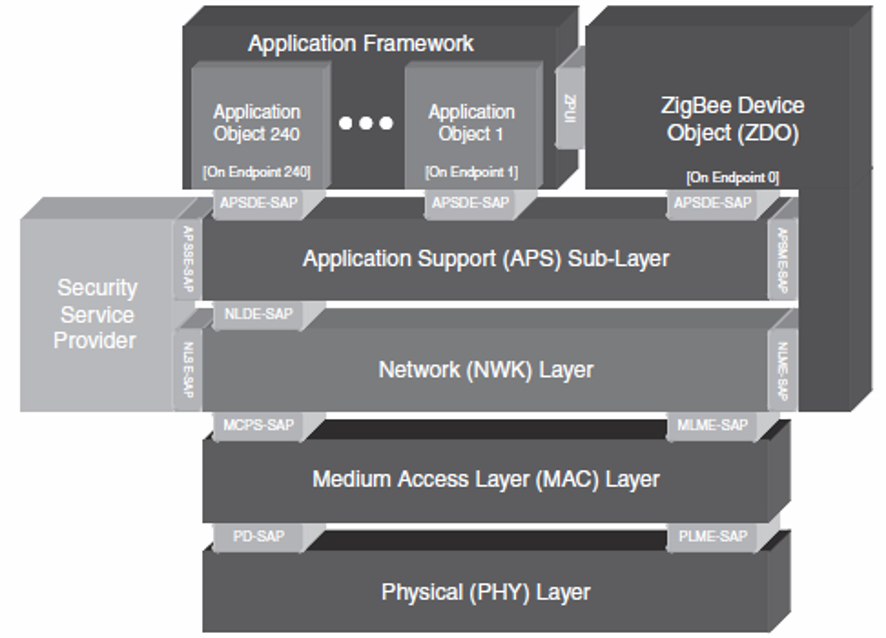
\includegraphics[scale=0.6]{a_zigbee.png}
	\caption{Zásobník ZigBee architektúry.
	\cite{gislason2008zigbee}}
	\label{f:o_zigbee_stack}
\end{figure*}

\begin{figure*}[h]
	\centering
	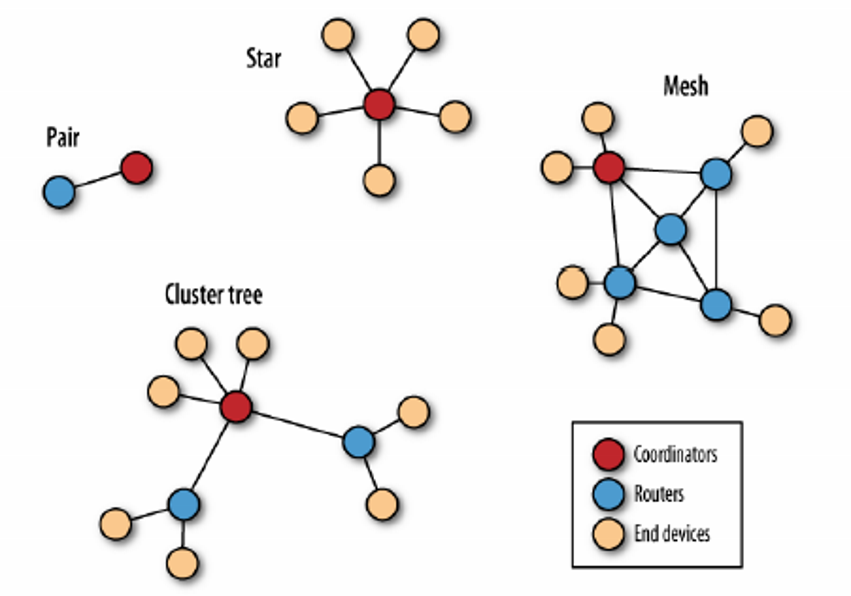
\includegraphics[scale=0.4]{a_zigbee_topologies.png}
	\caption{Možné topológie sietí s použitím ZigBee protokolu. \cite{faludi2010building}}
	\label{f:o_zigbee_topology}
\end{figure*}

%book zigbee
\singlespacing
\begin{table}
	\caption{Výhody a nevýhody jednotlivých ZigBee topológií. \cite{zigbeebook}} 
	\label{table:zigbee_arch}
	\begin{tabularx}{\textwidth}{|c|Y|Y|}
		\hline
		\textbf{Topológia} & \textbf{Výhody} & \textbf{Nevýhody} \\
		\hline
		\textbf{Star} & 
		\singlespacing
		\begin{itemize}
			\item Jednoduchá synchronizácia,
			\item podpora nízkého výkonu,
			\item malá odozva,
		\end{itemize}
		&  
		\begin{itemize}
			\item malá rozšíriteľnosť.
		\end{itemize}
		\\
		\hline
		\textbf{Tree} & 
		\begin{itemize}
			\item Nízke nároky na routovanie,
			\item možnosť vytvárať superframy s podporou sleep režimu,
			\item podpora pre multi-hop komunikáciu.
		\end{itemize}
		&
		\begin{itemize}
			\item Rekonštrukcia cesty je náročnejšia na prostriedky,
			\item môžu vznikať väčšie odozvy.
		\end{itemize}
		\\
		\hline
		\textbf{Mesh} &
		\begin{itemize}
			\item Robustná multi-hop komunikácia,
			\item sieť je pružnejšia na prispôsobenie,
			\item malé odozvy.
		\end{itemize} & 
		\begin{itemize}
			\item Nemožnosť vytvárať superframy, nepodporuje ani sleep režim,
			\item vyhľadávanie cesty je výpočtovo náročné,
			\item väčšie nároky na routovacie tabuľky.
		\end{itemize} \\
		\hline
	\end{tabularx}
\end{table}
\onehalfspacing

\begin{figure*}[h]
	\centering
	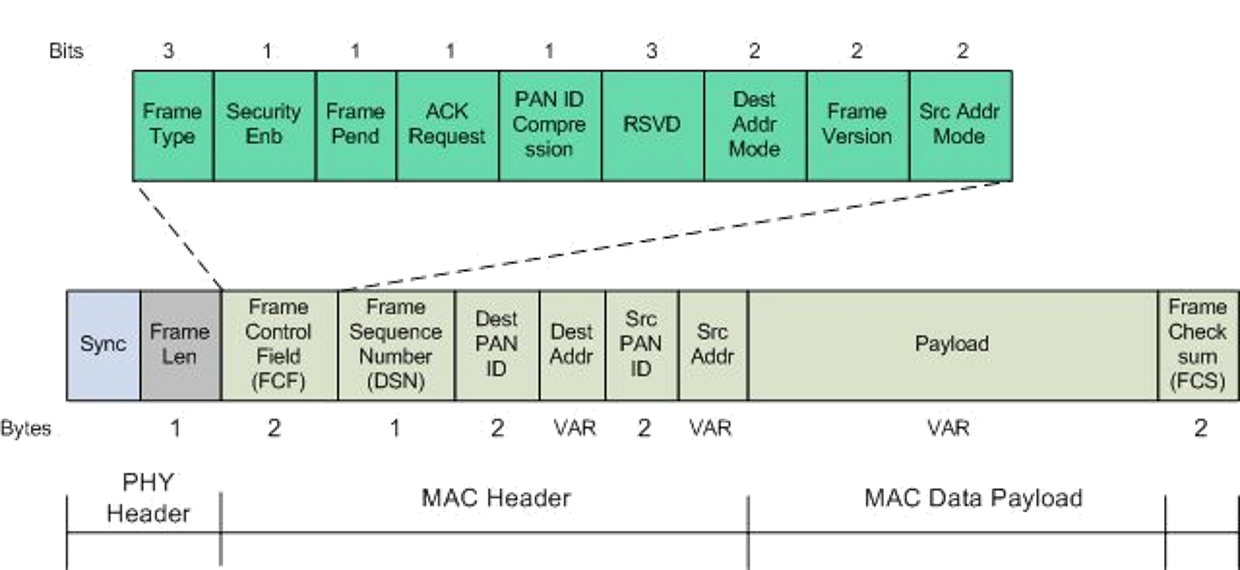
\includegraphics[scale=0.4]{a_zigbeepacket.png}
	\caption{Formát paketu 802.15.4 PPSDU. \cite{zigbeepacket}}
	\label{f:o_zigbee_packet}
\end{figure*}

%http://fosiao.com/content/zigbee-and-wifi-rf-channels
Všetky pásma používajú tzv. DSSS Direct Sequence Spread Spectrum prístup. \footnote{\url{http://www.ni.com/white-paper/4450/en/}}
\begin{figure*}[h]
	\centering
	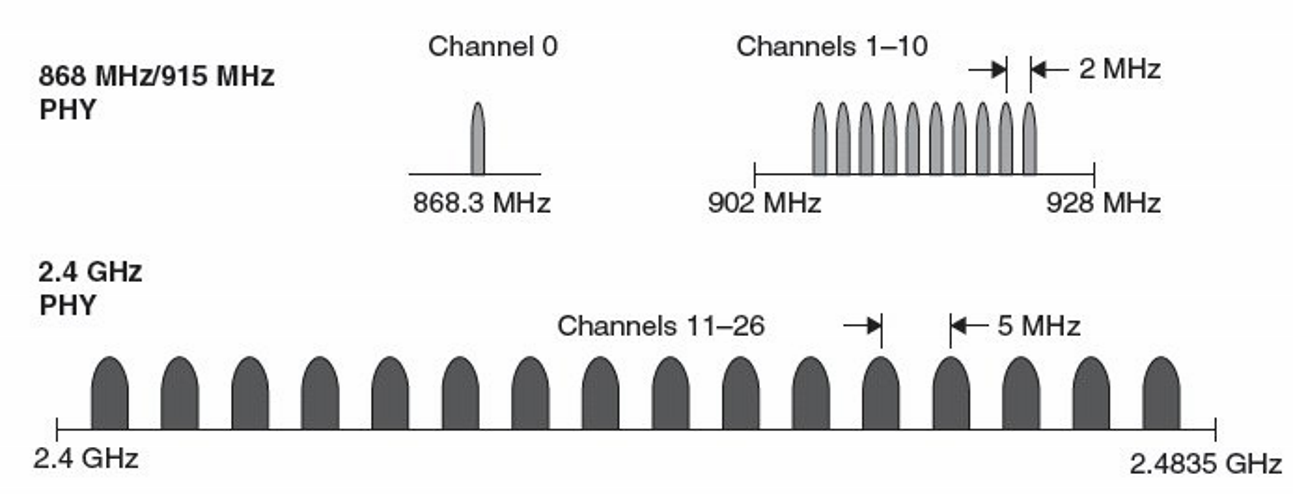
\includegraphics[scale=1]{a_zigbee_bands.png}
	\caption{Prenosové pásma protokolu ZigBee pre rôzne krajiny. \cite{zigbeebands}}
	\label{f:o_zigbee_bands}
\end{figure*}

%TODO Analýzou zraniteľsností ZigBee protokolu, bola zistená bezpečnostná slabina ktorá spočíva v nezmenených preddefinovaných kľúčoch, kde útočník zarušením prenosového komunikačného pásma a následneho spárovania cieľového zariadenia s útočníkovým uzlom, vie získať Network Key v nešifrovanej podobe a tým sa pripojiť do cieľovej siete. Tým, že je robená autentizáciu na aplikačnej úrovni pomocou PKI sa vyhneme podvhrnutiu, modifikácií a falšovaniu správ. Útočník však vie realizovať útok na koncové uzly a zahlcovať ich neautentifikovanými správami. V ďalšej fáze sa pozrieme na navrhované bezpečnostné mechanizmy, ktoré by mali predísť tomuto problému. \cite{zigbeeexploit} \footnote{\url{https://www.blackhat.com/docs/us-15/materials/us-15-Zillner-ZigBee-Exploited-The-Good-The-Bad-And-The-Ugly-wp.pdf}}

\subsection{IEEE 802.15}
Štandardy ako NFC alebo RFID sú použiteľné napr. na identifikáciu ľudí alebo zariadení v objekte. Pomenej sa v inteligentných domácnostiach zvyknú používať aj siete typu MAN alebo UWB (Ultra Wide Band).
Na aplikačných vrstvách štandardu 802.15 sa zavádzajú rôzne služby ako IPv6 adresovanie, definované podľa štandardu 6LoWPAN. alebo sa snažia zjednodušiť prenos dát v ľudsky čitateľnej forme, ako je tomu pri protokole CoAP (Constrained Application Protocol). Ten umožňuje prenášať dáta vo forme JSON alebo XML. Na zabezpečenie používa mechanizmus DTLS (Datagram Transport Layer Security).

\subsection{X-10}
X-10 je komunikačný protokol, ktorý bol pôvodne navhrnutý na prenos signálov prenášaných po napäťovej elektroinštalácii s napätím 120 V. Protocol X-10 používa 120 kHz dávky, ktoré sú synchronnizované na prechod fázy nulou\footnote{\url{http://www.johnloomis.org/ece445/topics/x-10/x10.html}} s elektrickým vedením, tak aby reprezentovali digitálnu informáciu. Dostupné sú produkty od rôznych výrobcov, ktoré spolu navzájom vedia komunikovať a umožnujú automatizáciu.\cite{x10mi}
Neskôr sa protokol presunul aj na bezdrôtový komunikačný kanál. Štandard funguje na dvoch frekvenčných pásmach: 433.29 MHz a 310 MHz. \cite{x10freq}

\subsection{Insteon}
Protocol navrhnutý spoločnosťou Insteon umožňuje prenos dát po bezdrôtovej a drôtových komunikačných linkách, napr. v prípade výpadku bezdrôtového komunikačného média.
Dáta na elektrickom vedení sa prenášajú na nosnej frekvencií 131.65 kHz. Nosná frekvencia RF bezdrôtového komunikačného kanála je 915 MHz.
Po stránke zabezpečenia ponúka maskovanie adries, čím schováva topológiu a ponúka aj kryptovanie dát. \cite{insteon}
%\subsection{KNX}
%\subsection{UPB} universla power line buss

\subsection{Lutron ClearConnect RF}
Protokol je vyvinutý spoločnosťou Lutron, ktorý slúži hlavne pre automatizáciu a poprepájanie osvetlenia so zabezpečením maximálnej možnej spoľahlivosti. Protokol využíva prenosové pásmo na frekvencií 400 MHz. Systém podporuje obojsmernú RF komunikáciu, Dual frequency. Základné udávané parametre protokolu \cite{lutron}:
%\singlespacing
\begin{itemize}
	\item Zariadenia môžu vysielať nepretržite,
	\item celý systém je riadený udalosťami v systéme,
	\item architektúra a topológia siete je daná fixne, čím urýchľujú prenos dát v sieti,
	\item možnosť riadiť a komunikovať s viacerými zariadeniami v skupine.
\end{itemize}
\onehalfspacing

\subsection{ANT}
ANT je bezdrôtový komunikačný protokol na pásme ISM o frekvencií 2.4 GHz. Protokol je navrhnutý pre nízko-napäťové aplikácie, Podporuje niekoľko rôznych topológií. Topológie sú zobrazené na obrázku \ref{f:a_ant_network_types}. Komunikačný protokol je navrhnutý aby odolal elektromagnetickému rušeniu z okolia, aby sa dal ľahko adaptovať a podporuje spoľahlivú komunikáciu.
S ANT modulom sa komunikuje pomocou sériovej komunikácie a na implementáciu architektúry postačuje 8 bitový mikropočítač.

Protokol ANT podporuje niekoľko typov komunikačných kanálov:
\begin{itemize}
	\item bidirectional: zariadenie definuje, +že bude komunikačný kanál využívať obosjmerne. Primárne však zadefinuje, či preferuje skôr uplink alebo downlink,
	\item shared bidirectional: sa používa na komunikáciu po jednom komunikačnom kanále s centralizovaným uzlom,
	\item receive only, transmit: umožnuje jednosmernú komunikáciu s uzlom. Zariadenie vie napr. posielať správy typu broadcast, ale nemôže prijímať potvrdenia správ.
\end{itemize}

\begin{figure*}[h]
	\centering
	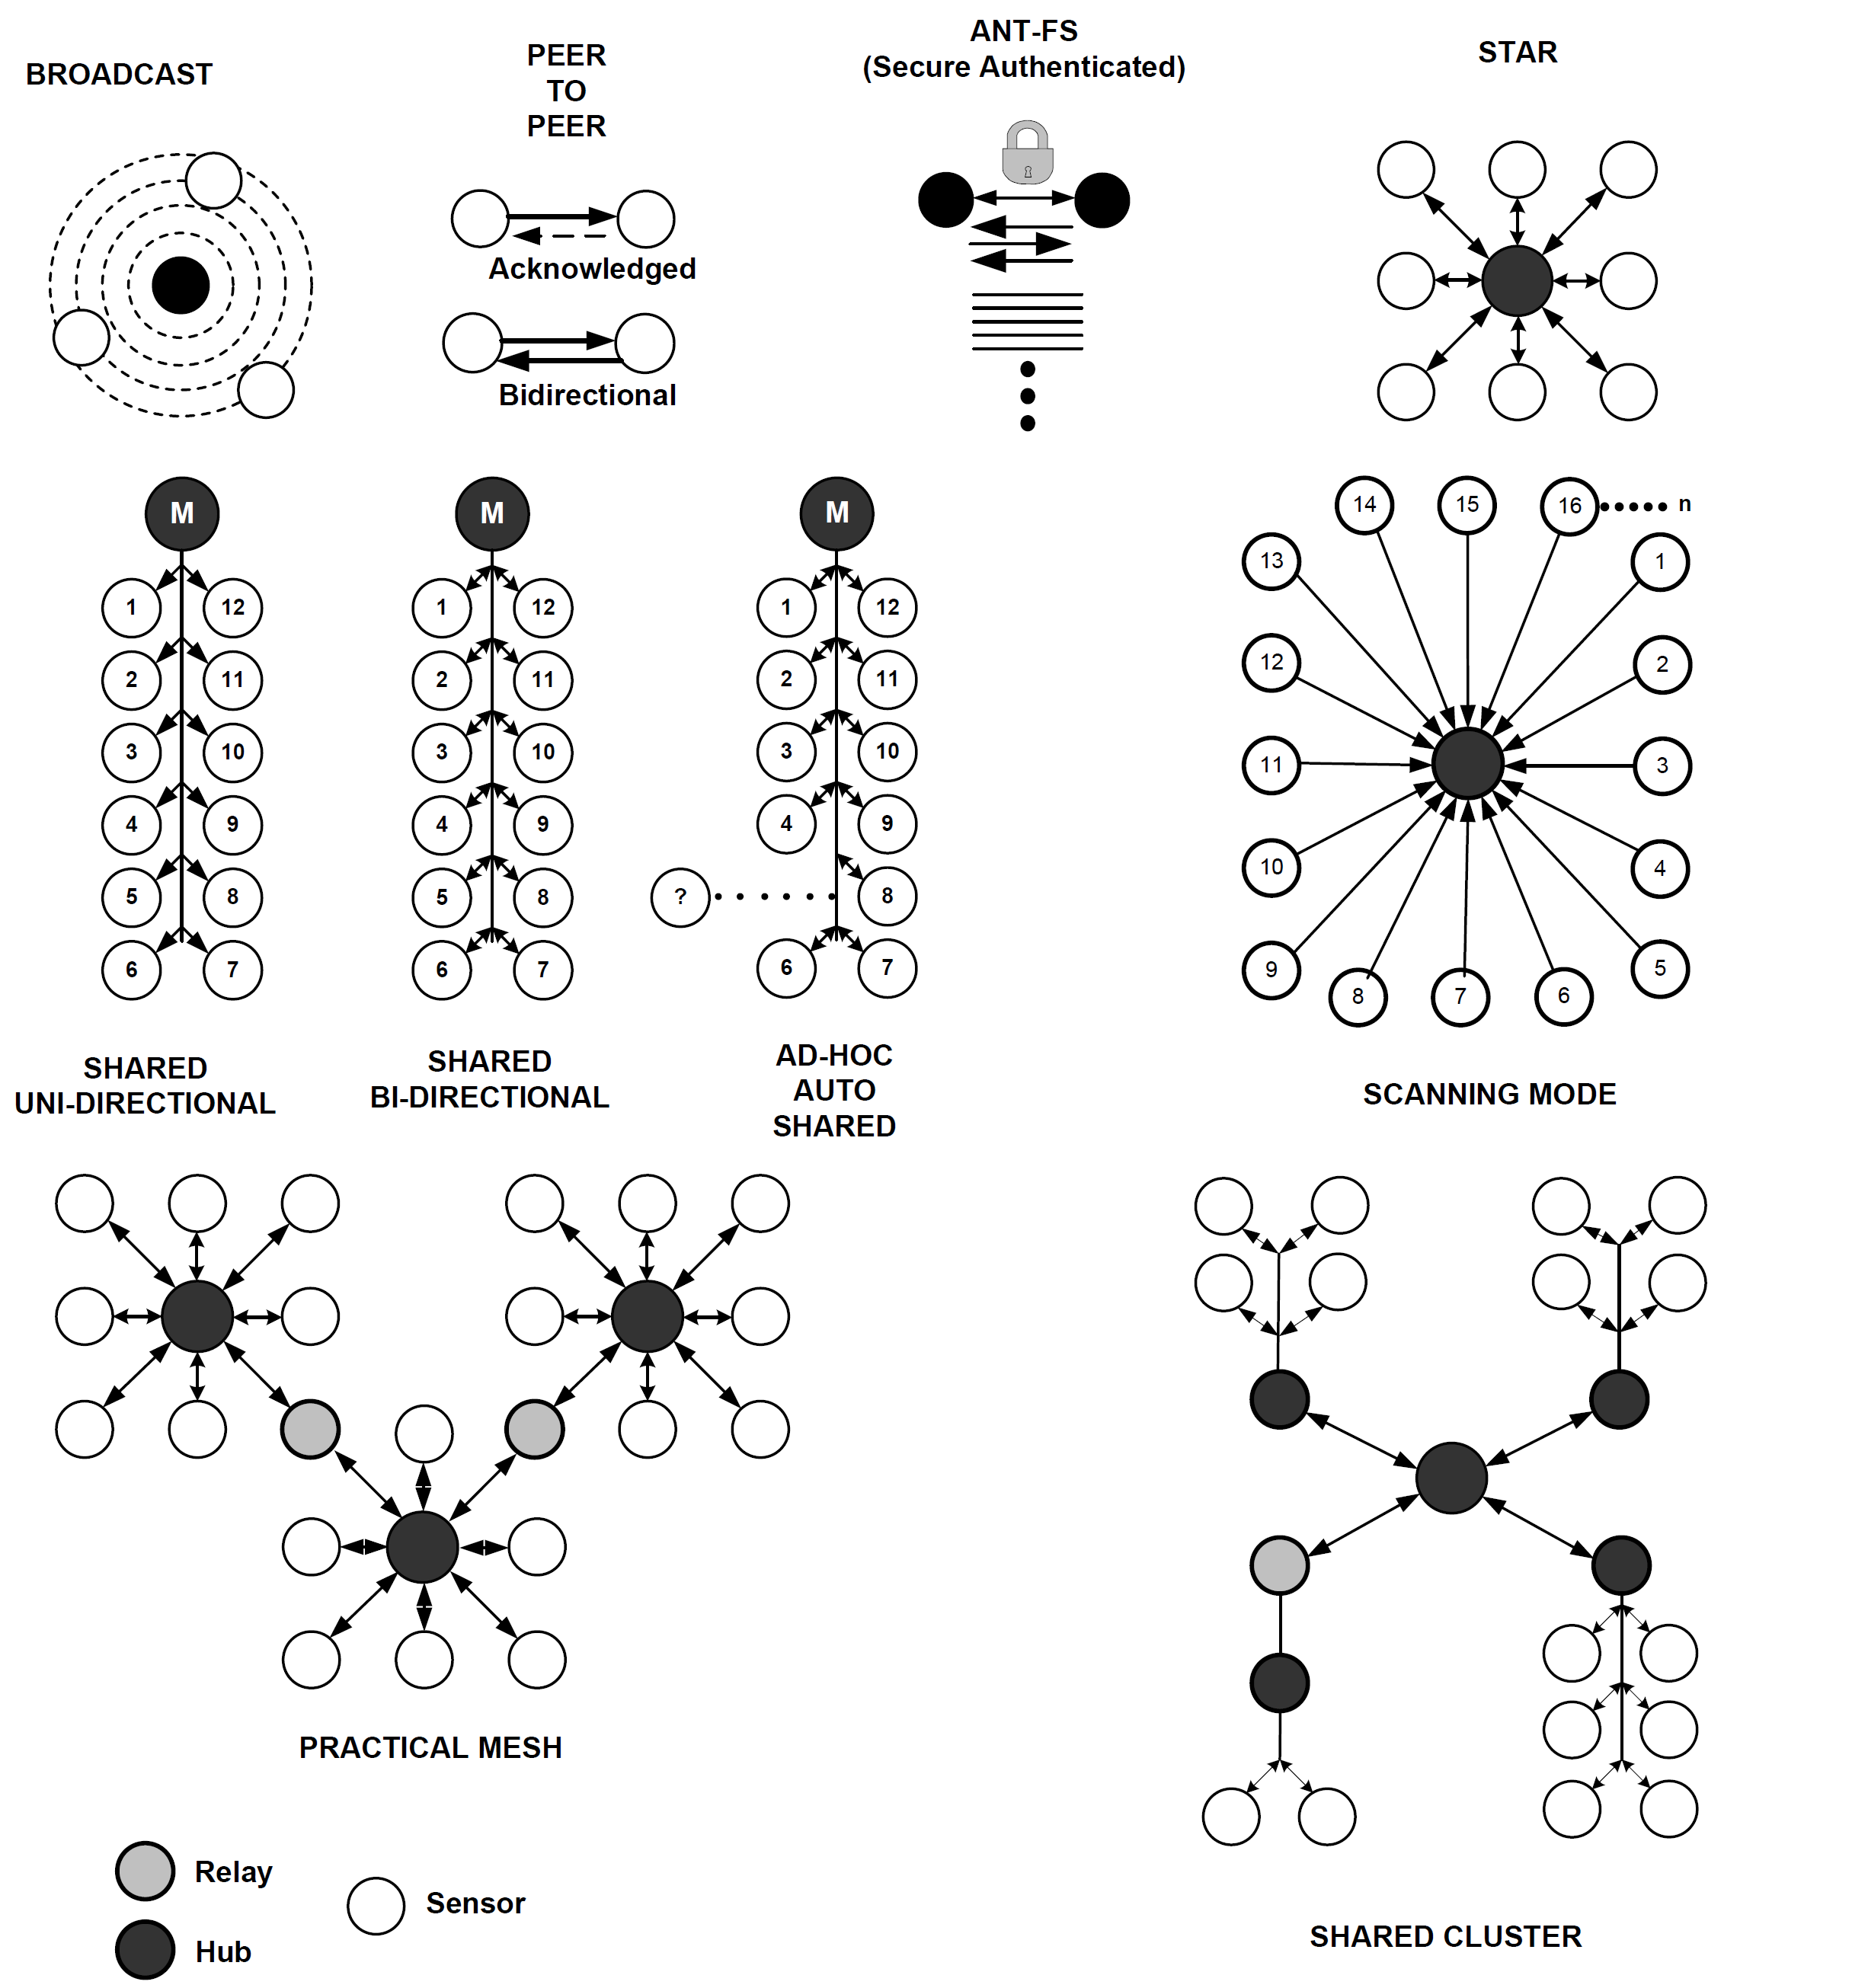
\includegraphics[scale=0.13]{ant_structures.png}
	\caption{Podporované topológie protokolu ANT.\cite{ANT}}
	\label{f:a_ant_network_types}
\end{figure*}

ANT protokol definuje 3 typy sietí, v ktorej každý typ môže definovať sadu pravidiel, ktoré musia uzly na danej sieti \cite{ANT}:
\begin{itemize}
	\item verejné: tento typ sietí vie zabezpečiť, že sieť je verejne dostupná, alebo zámerne zdieľaná medzi rôznymi výrobcami.
	\item privátne siete sa snažia zabezpečiť bezpečnosť siete a obmedzenie prístupu iba vybraných zariadení.%zariadenie mozu byt rozdelene do  kanalov viacerych roznych sieti
	\item manažované, ANT+ alebo ANT-FS siete. Zariadenia v tomto type sietí zabezpečujú vzájomnú štandardizáciu, interoperabilitu a kompatibilitu.
\end{itemize}
\onehalfspacing

ANT protokol podporuje 4 typy posielaných správ \cite{ANT}:
\begin{itemize}
	\item Broadcast: je najjednoduchší typ správy, ktorý sa posiela od Master zariadenia smerom ku všetkým Slave zariadeniam. Správy typu broadcast nie sú nikdy potvrdzované. Tento mód spotrebuváva najmenej elektrickej energie.
	\item Potvrdzované správy: na obojsmernej linke, zariadenie vie poslať potvrdenie o prijatí správy v ďalšom voľnom časovom slote. Treba však mať napamäti, že správa sa automaticky nepošle znova pri neprijatí správy o úspešnom prijatí. Tento komunikačný mód spotrebuváva viac energie a prenosového pásma.
	\item Burst: umožnuje posielať väčšie množstvo dát jednému uzlu v sieti. Tento mód je potvrdzovaný o úspešnom prijatí celého bloku dát.
	\item Advanced burst je rovnaký ako burst mód, s jediným rozdielom vo väčšej rýchlosti prenosu dát medzi uzlami blížiacich sa až k 60 kbps.
\end{itemize}
\onehalfspacing

Formát najzákladnejšej správy na ANT protokole je na \ref{f:a_ant_message}. Synchronizačná postupnosť bitov je 10100100. Kontrolná suma je počítaná ako XOR všetkých predošlých bajtov v správe \cite{ANT}.

\begin{figure*}[h!]
	\centering
	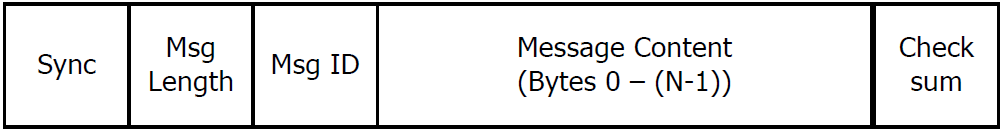
\includegraphics[scale=0.3]{a_ant_message_structure.png}
\caption{Najjednoduchší formát správy protokolu ANT\cite{ANT}.}
\label{f:a_ant_message}
\end{figure*}

\subsection{LoRaWAN, LoRa}
Označenie LoRa (Long Range) definuje spôsob modulácie pre bezdrôtovú komunikáciu, ktorá vznikla za účelom komunikácie na väčšiu vzdialenosť, batériami napájaných zariadení a s podporou veľkého počtu zariadení v sieti. Jedná sa o fyzické rozhrania PHY. Technika modulácie je odvodená od CSS (Chirp Spread Spectrum) a obsahuje doprednú korekciu chyby (FEC). Z takto zakódovaného signálu sme schopný extrahovať informáciu, aj keď je prijatý signál žašumený a oslabený na úroveň -19.5 dB pod hranicou šumu.

Štandardu LoRa je často porovnávaný so sieťou IoT od poskytovateľa s názvom SigFox. Topológia použitá pre štandard LoRa je star. Tým by sa mala zabezpečiť vyššia kapacita siete, nižšia spotreba a väčší dosah\cite{LoRaSpec}\cite{LoRaFAQ}.

Tento štandard sa zaraďuje do kategórie LPWAN Low-Power Wide Area Network. 

Štandard LoRa používa na komunikáciu bezplatné ISM pásmo frekvenčných pásmach Sub-GHz. Tým sa zaručí nižšia cena zariadení, keďže niesú potrebné licenčné poplatky. Navyše sa vyhýbajú frekvenčným pásmam 2.4 GHz, na ktorých operuje v dnešnej dobe veľa zariadení a stávajú sa preplnenými. Vyhradené frekvencie pre jednotlivé regióny sú na obrázku \ref{f:a_LoRaWAN}.

LoRaWAN označuje MAC (Media Access Control) nad fyzickým rozhraním LoRa a definuje komunikačný protokol, formáty posielaných správ a samotnú architektúru siete.

V LoRa sieti zariadenia patria do jednej siete. Odoslaná správa od jedného zariadenia môže byť prijatá a spracovaná viacerými bránami. Pri poruche jednej brány bude správa doručená cez iný, ktorý počúva na tej istej frekvencií, v závislosti od regiónu \ref{f:a_LoRa_Architecture}. Brány sú rozmiestňované tak, aby sa navzájom čiastočne prekrývali.

LoRaWAN štandard je orientovaný pre cloudové aplikácie. Správy prijaté v jednotlivých bránach sú ďalej preposielané severu na spracovanie po inom komunikačnom kanále\ref{f:a_LoRa_Architecture}.
Správy štandardu LoRa sú rôzne pre uplink a downlink.

Štandard používa na zapezpečenie spoľahlivého prijatia metódu ADR (Adaptive data rate)\ref{f:a_LoRa_ADR}. Prenosová rýchlosť a vysielací výkon zariadenia sa prispôsobujú vzdialenosti, alebo počtu zariadení v sieti. Takýmto spôsobom sa dá zaručiť efektívne nakladanie s kapacitou batérie. Prenosové rýchlosti pri modulácií LoRa sa pohybujú v rozmedzí 0.3-50 kbps a pri modulácií GFSK 100 kbps \cite{LoRaFAQ}.

Zariadenia v štandarde LoRa sú rozdelené do troch kategórií, kvôli rôznym nárokom a požiadavkám na uzly:
\begin{itemize}
	\item kategória A (All-end devices): uzly tejto kategórie sú napájané batériami. Zvyčajne sa jedná o senzory. Prijímanie správ je možné iba v 2 časových úsekoch po odoslaní dát. Keďže zariadenie sú zvyčajne v režime šetriacom a nemajú zapnuté. Umožňuje im to uspať a prijať dáta, ak si ich zažiadali alebo ich očakávajú.
	\item kategória B (Beacon): do tejto kategórie patria aktuátory napájané batériami. Komunikácia s takýmito zariadeniami je synchronizovaná v časových úsekoch a umožnuje viac prijímacích okien.
	\item kategória C (Continuously listening): jedná sa o zariadenia napájané z elektrickej siete, ktoré môžu počúvať na komunikačnom kanále nepretržite s výnimkou vysielania.
\end{itemize}

Zabezpečenie je dvojúrovňové, pomocou kryptosystému AES. Prvá úroveň je na aplikačnej úrovni, ktorá zabezpečuje dôvernosť prenášaných dát cez sieť. Druhá úroveň je na sieťovej úrovni.

Pokiaľ je posielaná správa od koncového uzla zachytená aspoň tromi bránami je možná geolokácia s príslušnou presnosťou. LoRaWAN štandard sa dá aplikovať aj na menšie privátne siete, na rozdiel od siete SigFox.
%Problem pri pohybe a posielaní

\begin{figure*}[!htb]
	\centering
	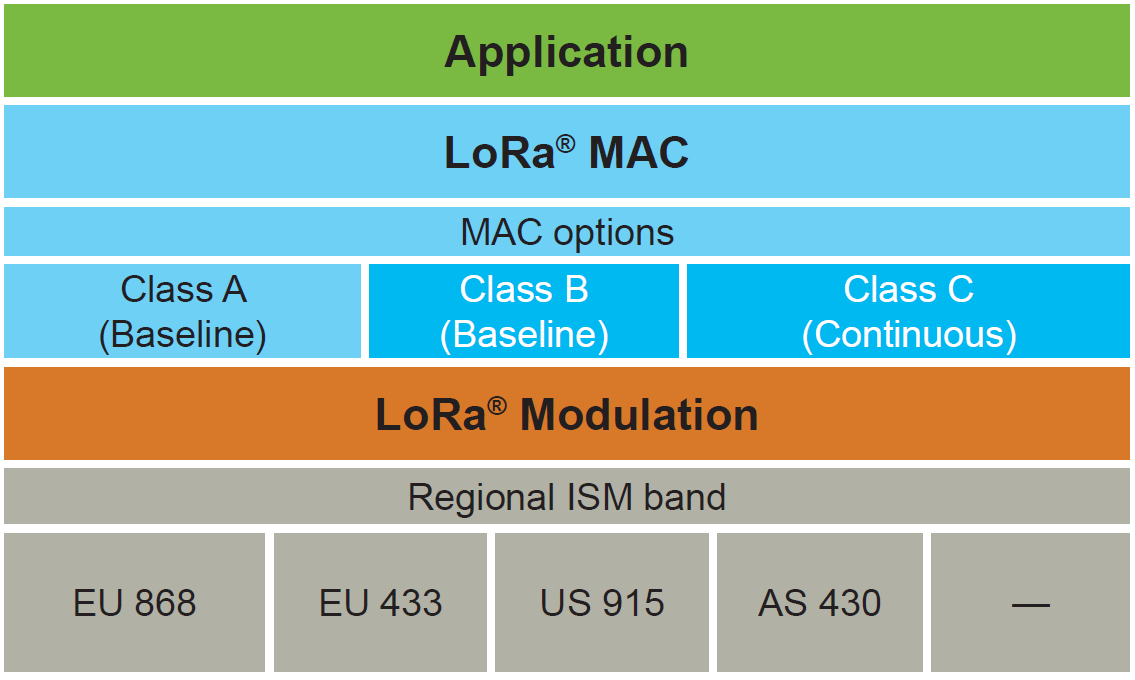
\includegraphics[scale=0.22]{LoraWAN.png}
	\caption{Architektúra LoRaWAN\cite{LoRaOverview}.}
	\label{f:a_LoRaWAN}
\end{figure*}


\begin{figure*}[!htb]
	\centering
	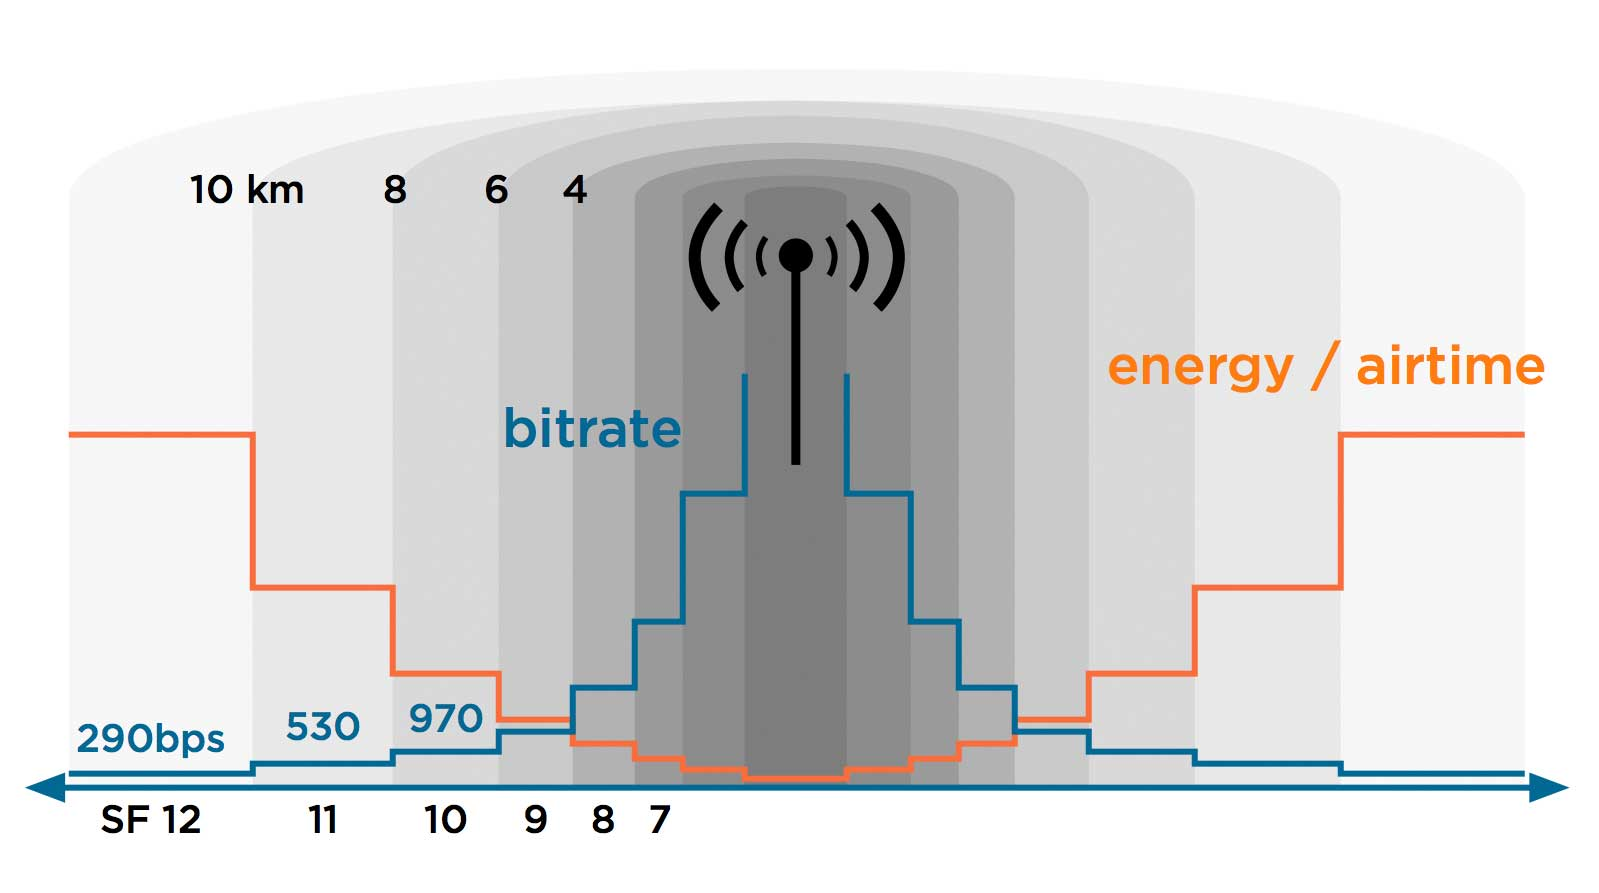
\includegraphics[scale=0.2]{a_LORA_VBR_adr.jpg}
	\caption{Prispôsobovanie výkonu a prenosovej rýchlosti v závislosti od vzdialenosti komunikujúcich uzlov.\cite{LoRa_VBR}}
	\label{f:a_LoRa_ADR}
\end{figure*}

\begin{figure*}[!htb]
	\centering
	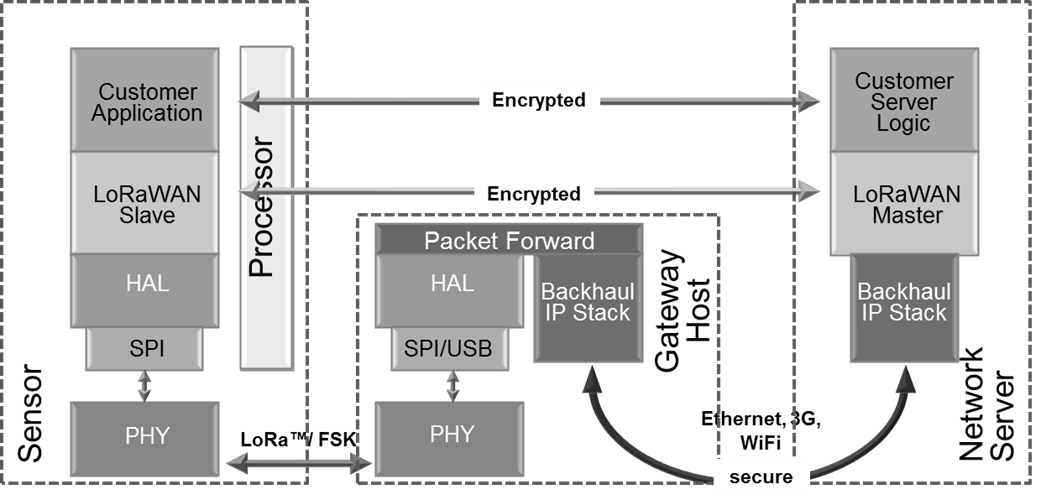
\includegraphics[scale=0.7]{a_LORA_networkBW.png}
	\caption{Infraštruktúra LoRaWAN\cite{LoRa}.}
	\label{f:a_LoRa_Architecture}
\end{figure*}

\section{Porovnanie protokolov}
%TODO
V závislosti na veľkosti siete a počtu uzlov v sieti, nie je každý protokol najvhodnejší. Na veľmi malé priestory v podobe malých jednopodlažných firiem sa najviac hodí protokol BLE napr. v prevedení piconet.
Na malé viacpodlažné domčeky s menšou predzáhradkou, niektorý so štandardov 802.15.4 napr. Zigbee.
Na väčšie domy s vlastnými farmami, niekoľkými budovami, s veľkými záhradami a poliami a na priemyselné použitie vo veľkých fabrikách sa hodí protokol LoRa.
Viaceré protokoly sú spolu porovnané v tabuľke \ref{table:Porovnanie protokolov}.
%Celulárne riešenia sa mi nepacia, potrebujes poskytovatela, musis mu platit za architekturu, nemusi mat pokrytie, handovery, znizena bezpecnosti.

\begin{table}[H]
	\centering
	\caption{Porovnanie jednotlivých parametrov vybraných protokolov.}
	\label{table:Porovnanie protokolov}
	\Rotatebox{90}{
		\begin{tabularx}{\textwidth}{|X|p{1.5cm}|p{1.5cm}|p{2cm}|p{2.4cm}|p{1.8cm}|p{2.4cm}|}\hline
			\textbf{Protokol} & \textbf{Výkon} & \textbf{Range} & \textbf{Data rate} & \textbf{Frekvencie} & \textbf{Devices} & \textbf{Security}  \\ \hline 	% &  & \textbf{Stack req.}  modulacia cena za jednotku
			\textbf{NFC} &  & 20cm  & 26 - 848kb/s & 13.56 MHz & 2  &  \\ \hline
			\textbf{ANT} & 2.5 mW  &  300m & 60 kbps & 2.4GHz  & 65535  &  AES-128\\ \hline % 8 bit newtork 16 bit devid 4dbM
			\textbf{Bluetooth} & 1/2.5/ 100mW & 10cm/ 10/100m & 24Mb/s & 2.4GHz & 7  & SSP, 16B PIN, ECDH, AES-CMAC, $E_0$\\ \hline
			\textbf{Zigbee} & 1mW-1W & 100m  & 250 kb/s &  2.4GHz, 915MHz 868MHz & 65535 & AES-128\\ \hline
	    	\textbf{WiFi} & 30 mW-250mW & 38-250m &  1-2,54,248 Mb/s & 2.4, 4.9, 5 GHz & 30-60 & AES-CCMP\\ \hline % WPA2 PSK preshared  key a lebo eap
	    	\textbf{LoRa} & 25mW - 1W & 2-22km & 250b/s- 50kb/s & 868, 433 915 430 MHz &  $2^{25}$ & AES-128\\ \hline
	    	\textbf{GSM} & 1W, 2W & 31 km  & 9.2 kb/s & 850, 9**, 1900 MHz &  & COMP128\\ \hline % 380, 4**, 7**, MHz, TMSI
	    	\textbf{LTE} & 200mW  & 13 - 100 km &  10 - 100 Mb/s & 700-2600 MHz &  & 128-EEA EIA \\
		\hline \end{tabularx}
	}
\end{table}

%http://www.sharetechnote.com/html/Handbook_LTE.html

\section{Používané technológie v inteligentných domácnostiach} \label{s_solutions}
Táto kapitola sa zaoberá dostupnými a používanými technológiami používanými v technologických riešeniach inteligentných domácností.  \ref{s_smarthubs} a \ref{s_devices}
\subsection{Smart gateways} \label{s_smarthubs}
Smart gateways, často označované a dostupné na internete aj pod názvom Smart Things Hubs, označujú zariadenia, ktoré sú pripojené k internetu a poskytujú konektivitu pripojeným senzorom, ktoré nemajú priamo zabudované pripojenie k internetu. Takýmto spôsobom je možné monitorovať a ovládať dianie v inteligentnej domácnosti pomocou vzdialeného prístupu, posielať namerané dáta von z privátnej siete napr. do cloudu na následné spracovanie alebo notifikovať vlastníka objektu o narušiteľovi, poprípade o spustení požiarneho alarmu. Okrem pridanej konektivity často vedia komunikovať a prepájať zariadenia nachádzajúce sa na rôznych bezdrôtových komunikačných protokoloch.
Vybrané najrozšírenejšie dostupné produkty:
%\singlespacing
\begin{itemize}
	\item Icontrol Networks Piper,
%	\item SmartThings Hub,
	\item Samsung SmartThings hub,
	\item Bee-wi,
	\item Icontrol Networks Piper,
	\item Logitech Harmony Home Hub,
	\item Lutron Smart Bridge.
\end{itemize}
\onehalfspacing

\begin{figure*}[h]
	\centering
	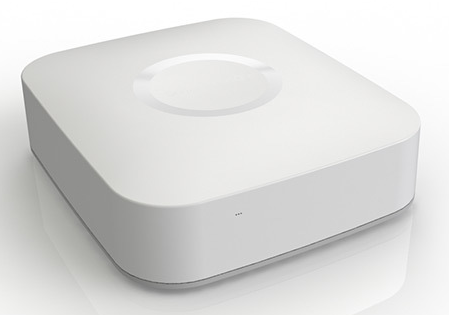
\includegraphics[scale=0.5]{a_hub.png}
	\caption{Samsung SmartThings hub.\cite{hub}}
	\label{f:o_hub}
\end{figure*}
\subsection{Dostupné produkty} \label{s_devices}
Na trhu sú dostupné a predávané rôzne zariadenia, ktoré používateľovi umožňujú ručné prispôsobenie nastavení, automatizáciu alebo monitorovanie zariadení, či už prostredníctvom univerzálnejších centralizovaých riadiacich jednotiek, alebo pomocou mobilných applikácií.
Pre priblíženie spomenieme zopár zariadení spolu so stručným popisom ponúkanej funckionality:
%\singlespacing
\begin{itemize}
	\item Belkin Wemo Internet Wall plug: umožňuje prostredníctvom Wifi pripojenia vypínať a zapínať pripojené zariadenia,
	\item GreenWave Reality Smart Bulb: nastaviteľná a ovládateľná žiarovka,
	\item Phillips Hue: ponúka používateľovi prispôsobenie osvetlenia,
	\item Winkhub produkty: spoločnosť sa venuje predávaniu žiaroviek, LED diódových pásov, vypínačov, zásuviek, detektorov pohybu a úniku vody, zámkov alebo termostatov, s ktorými používateľ komunikuje pomocou bezdrôtového komunikačného kanála.
\end{itemize}
\onehalfspacing
%\subsection{Microchip IoT, TexasInstruments}

%Kupim riesenie,
%Spajam od roznych vendorov
%Cele robim sam krabickovo,

%prudovy blokovy prenos
%QOS
%Detekcia compromitovaneho sensoru, observeri, watchdog
\subsection{Smart SD karty}
Nasledujúca podkapitola sa venuje opisu rozširujúcich sa hardvérových zariadení, ktoré ponúkajú funkcionalitu prevážne z oblasti zabezpečenia a konentivity, akými sú bezpečné ukladanie kryptografických kľúčov alebo citlivých dát.
Existujú aj SD karty, ktoré neponúkajú zvýšené služby zabezpečenia ale iba bezdrôtovú komunikáciu prostrednícvtom Wi-Fi protokolu a úložisko. Príkladmi daných kariet sú napr. SD karty s názvom Eyefi\footnote{\url{http://www.eyefi.com/}} a Transcend\footnote{\url{http://www.transcend-info.com/Products/No-401}}. Na trh sa snaží dostať aj spoločnosť Toshiba s NFC SDHC  kartou\footnote{\url{http://www.toshiba.com/taec/adinfo/technologymoves/pdfs/2015/World's\%20First\%20NFC\%20Built-in\%20SDHC\%20Memory\%20Card.pdf}}.

\subsubsection{Secure Element} \label{s_se}
Secure element alebo embedded secure element je zariadanie, ktoré je odolné proti modifikácií. Príklad použitia tejto technológie je napr. pri autetizácií, identifikácií, zabezpečovaní integrity, bezpečnom ukladaní dôverných a kryptografických dát. Rozlišujú sa tri typy secure elementov. Použité sú napr. aj v kreditných a debetných kartách, SIM kartách alebo TV smart kartách. \cite{gp}\cite{gemalto}
Existujú tri hlavné typy secure elementov:
%\singlespacing
\begin{itemize}
	\item UICC (Universal Integrated Circuit Card) je karta, používaná v sieťach typu GSM, podobná SIM karte,
	\item microSD,
	\item eSE (embedded Secure Element): je SoC, ktorý má širokospektrálne použitie v rôznych zariadeniach.
\end{itemize}
\onehalfspacing
%https://www.globalplatform.org/mediaguideSE.asp
%http://www.gemalto.com/iot/consumer-electronics/embedded-secure-element

\subsubsection{Java Card} \label{s_jc}
%http://pfa12.free.fr/doc_java/javacard_specifications/specs/jcvm/html/
%http://www.oracle.com/technetwork/java/index.html
%http://www.javacardforum.org
%http://www.gemalto.com/techno/javacard
Pod označením Java Card sa nachádza priemyselný štandard, ktorý bol vyvinutý spoločnosťou Sun Microsystems (dnešný Oracle). Tento štandard umožnuje aby aplikácie na báze Javy tzv. applety, mohli byť spustené na smart kartách. Výhody takýchto riešení sú v jej interoperabilite, prenositeľnosti kódu a zníženým hadvérovým nákladom pri tvorbe cieľového produktu.
Typické použitia Java Card technológie \cite{jcop}:
%\singlespacing
\begin{itemize}
	\item identifikácia pri fyzickom alebo logickom prístupe k objektom, zariadeniam alebo databázam,
	\item platobné karty,
	\item identifikačné karty,
	\item karty používané vo verejnej preprave,
	\item telekomunikáciach,
	\item komunikácia v sieťach typu M2M medzi strojom a strojom bez prítomnosti a asistencie človeka.
\end{itemize}
\onehalfspacing

\subsubsection{Java Card OpenPlatform} \label{s_jcop}
%http://www.smartcardsource.com/contents/en-ca/d9_JCOP-NXP-cards.html
%http://www.usmartcards.co.uk/cards/java-cards.html
%http://www.zurich.ibm.com/jcop/
Pojem JCOP zastrešuje implementáciu vnoreného bezpečnostného operačného systému, ktorý rozširuje funkcionalitu tradičných smart kariet. \cite{jcopz} 
%ftp://ftp.software.ibm.com/software/pervasive/info/JCOP_Family.pdf
Základné vlastnosti JCOP operačného systému sú \cite{jcop}:
\singlespacing
\begin{itemize}
	\item Podporuje kompatibilitu s nasledujúcimi štandardami:
	\subitem JavaCard 2.1.1,
	\subitem GlobalPlatform 2.0.1,
	\subitem EMV a ISO 7816,
	\subitem ISO 14443,
	\subitem 3GPP 03.19 a 11.14,
	\item na beh mu postačujú pomerne malé hardvérové nároky:
	\subitem 8-bitový mikropočítač,
	\subitem 48 kB pamäte ROM,
	\subitem uloženie používateľského appletu v ROM pamäti spolu s OS,
	\item poskytuje metódy:
	\subitem RSA (2048 bitov),
	\subitem kontaktné alebo bezkontaktné rozhranie,
	\item prenositeľnosť kódu.
	\item kompatibilitu medzi rôznymi priemyselnými technológiami:
	\subitem bankovníctve/EMV,
	\subitem telekomunikáciach/SIM,
	\subitem zdravotníctve/ID.
\end{itemize}
\onehalfspacing

\begin{figure*}[h]
	\centering
	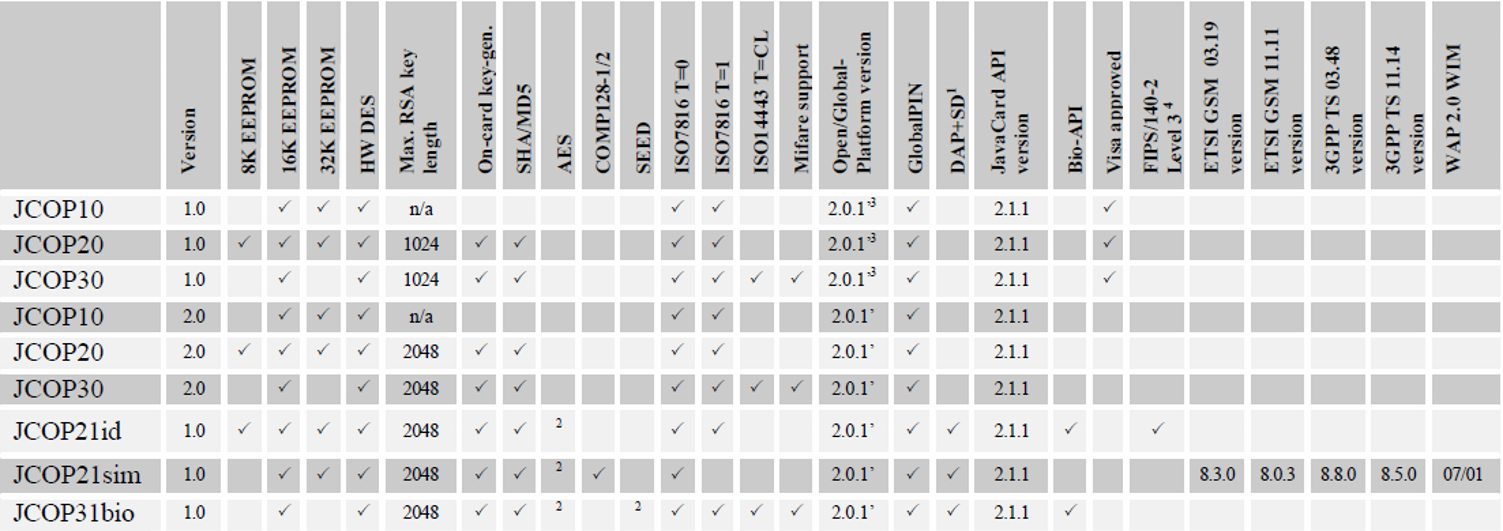
\includegraphics[scale=0.4]{s_jcop_versions.png}
	\caption{Verzie OS JCOP s vyznačenou podporou pre rôzne služby. \cite{jcop}}
	\label{f:o_jcop_0}
\end{figure*}
%
%\begin{figure*}[h]
%	\centering
%	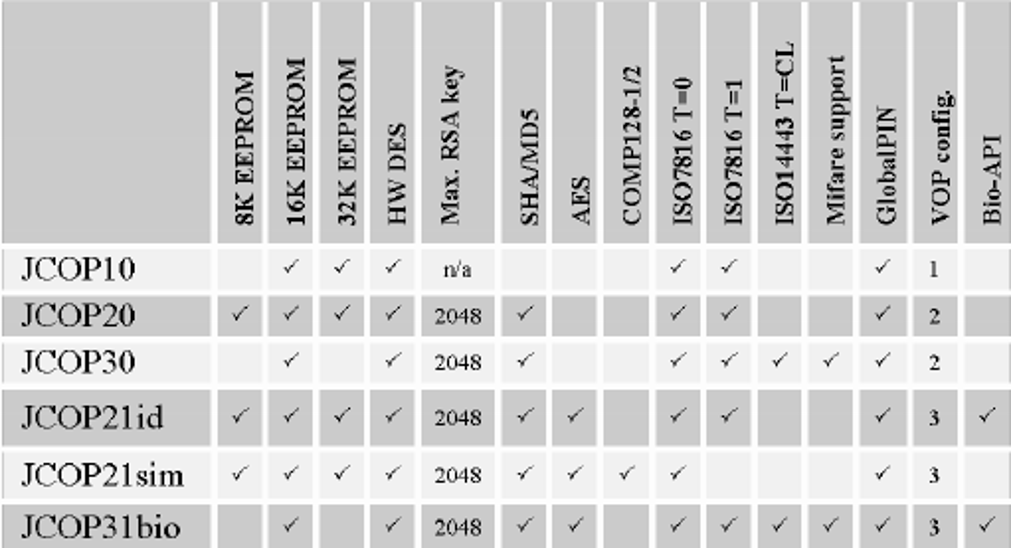
\includegraphics[scale=0.5]{s_jcop_versions0.png}
%	\caption{Verzie OS JCOP. \cite{jcop}}
%	\label{f:o_jcop_1}
%\end{figure*}

\subsubsection{Programovanie Secure Elementov}
Na programovanie secure elementov sa používa programovací jazyk so syntaxou Java a istými výraznými limitáciami zo strany inštrukčnej sady, služieb a podpory samotného virtuálneho stroja. Pre skompilovanie programu pre secure elementy je potrebné napr. vývojové štúdio Eclipse\footnote{\url{https://eclipse.org/}} spolu s nainštalovaným balíčkom JavaCard SDK\footnote{\url{http://www.oracle.com/technetwork/java/embedded/javacard/downloads/javacard-sdk-2043229.html}}.
Základná štruktúra programu je zobrazená na \ref{lst:jcop_program}. Program je nutné skompilovať do CAP formátu\ref{f:applet}.
Pre nahratie appletu na cieľovú smart kartu je ďalej potrebný manažér appletov napr. program od Global Platform s názvom GPShell\footnote{\url{https://sourceforge.net/p/globalplatform/wiki/GPShell/}}\ref{f:applet_install}. Následne je potrebné zariadenie, pomocou ktorého nahráte skompilovaný applet na smart kartu, napr. PCSC čítačku, ktorá komunikuje so Secure Elementom prostredníctvom štandardu a rozhrania ISO 7816.
% http://javacard.vetilles.com/2006/09/17/hello-world-smart-card/#sthash.gJ3w69ya.dpuf
%\singlespacing
\begin{lstlisting}[caption={Hello World na platforme JCOP. \protect\cite{jchelloworld}}, label={lst:jcop_program}, language=java] 
package com.vetilles.helloworld;
import javacard.framework.*;

public class HelloWorld extends Applet  {
  private final static byte[] hello = { 0x48, 0x65, 0x6c, 0x6c, 0x6f };
  public static void install(byte[] buffer, short offset, short length) {
    (new HelloWorld()).register();
  }
	
  public void process(APDU apdu) {
    byte[] buf = apdu.getBuffer(); 

      switch(buf[ISO7816.OFFSET_INS]) {
        case 0x40:
          Util.arrayCopy(
            hello,(byte)0,buf,ISO7816.OFFSET_CDATA,(byte)5);
          apdu.setOutgoingAndSend(
            ISO7816.OFFSET_CDATA,(byte)5);
          break;
       default:
        ISOException.throwIt(ISO7816.SW_WRONG_INS); 
    }
  }
}
\end{lstlisting}
\onehalfspacing

\begin{figure*}[h]
	\centering
	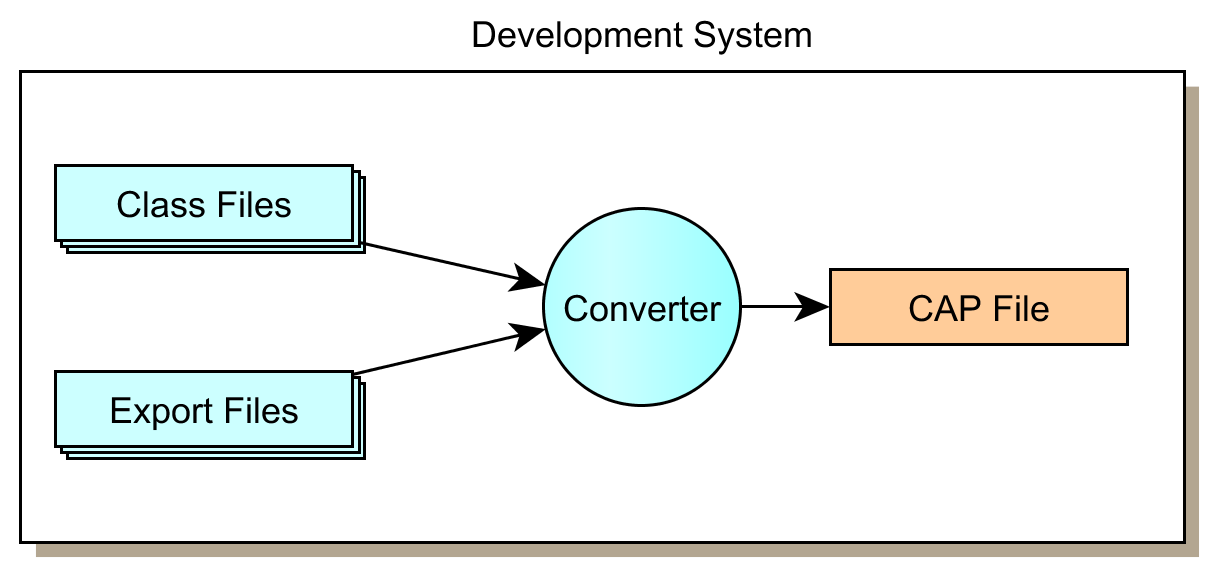
\includegraphics[scale=0.4]{applet.png}
	\caption{Kompilácia appletu do CAP formátu. \cite{javacardinstruction}}
	\label{f:applet}
\end{figure*}

\begin{figure*}[h]
	\centering
	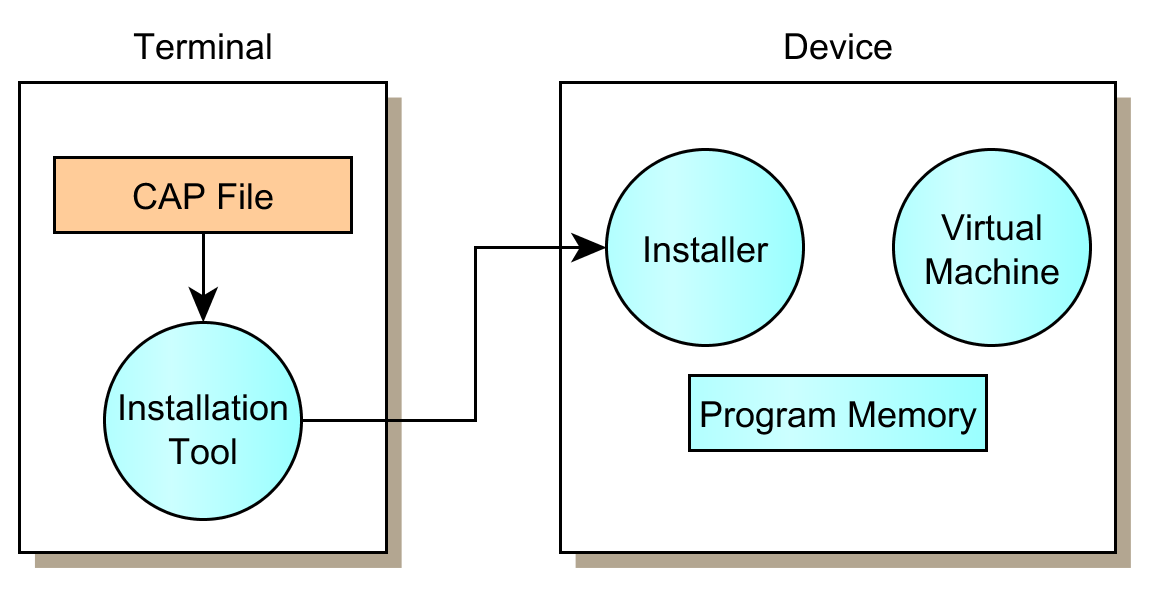
\includegraphics[scale=0.4]{applet_install.png}
	\caption{Inštalácia appletu na cieľové zariadenie. \cite{javacardinstruction}}
	\label{f:applet_install}
\end{figure*}

%https://www.sdcard.org/developers/overview/sdio/sdio_spec/Simplified_SDIO_Card_Spec.pdf
%http://alumni.cs.ucr.edu/~amitra/sdcard/Additional/sdcard_appnote_foust.pdf

Pri písaní programov pre Secure Elementy, treba mať napamäti, že spôsob, akým je napísaný samotný program ovplyvňuje aj výsledné zabezpečenie navrhovaného a implementovaného systému voči fyzickým útokom.
Vybrané odporúčania pri písaní appletov:
%\singlespacing
\begin{itemize}
	\item vkladať náhodné inštrukcie typu nop do vykonávaného programu,
	\item používať maskovanie hodnôt pri posielaní kritických parametrov funckiám napr. pomocou funkcie xor, bitových rotácií a ich následná rekonštrukcia,
	\item nepoužívať podmienené vetvenia, tie zvyknú byť náchylné na útoky hodinového signálu,
	\item pristupovať do ramky, nie do externých pamätí, vykonávanie programu je rýchlejšie a spotrebuje sa pri tom menej energie. Prístup do externých pamätí môže byť viditeľný pri útoku typu na postranný kanál,
	\item používať čo najviac zabudovaných služieb, ktoré sú overené a neimplementovať vlastné softvérové metódy,
	\item odpourúča sa programovať program tak, aby sa kód vykonával rovnaký počet hodinových cyklov v prípade v prípade správne zadanej používateľskej hodnoty aj pri zlej, napr. pri zadávaní pinu na hardvérovej klávesnici.
\end{itemize}
\onehalfspacing

Komunikácia s SD kartou pomocou štandardného rozhrania je možná pomocou dvoch hlavných módov\cite{sdio}:
\singlespacing
\begin{itemize}
	\item SD označovaný aj ako SDIO mód slúži na priamu komunikáciu, ten je možné realizovať po zberniciach s rôznou šírkou,
	\subitem 1-bitový synchrónny mód, umožňuje pomalší prenos informácií, šetrí sa však miesto na vyvíjanom čipe,
	\subitem 4-bitový synchrónny mód, rýchlejšia komunikácia s SD kartou,
	\item SPI mód podporuje jedno master zariadenie a viac slave zariadení. Tento mód podporuje iba menšiu množinu vykonávaných operácií nad SD kartou, ako je tomu pri SD móde.
\end{itemize}
\onehalfspacing

\begin{figure*}[h]
	\centering
	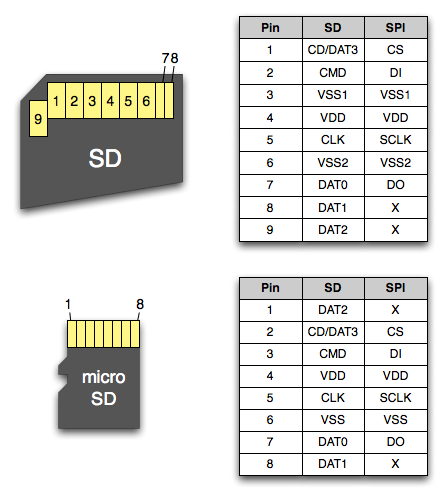
\includegraphics[scale=0.45]{a_sd-card-pinout.png}
	\caption{Rozmiestnenie pinov na SD a microSD karte. \cite{usdpinout}}
	\label{f:o_usd}
\end{figure*}

%http://www.cardwerk.com/smartcards/smartcard_standard_ISO7816-3.aspx komunikacia
\begin{figure*}[h]
	\centering
	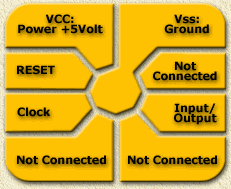
\includegraphics[scale=0.5]{iso7816pinout.png}
	\caption{Rozhranie štandardu ISO7816. \cite{iso7816pinout}}
	\label{f:o_ISO7816}
\end{figure*}
%sd usd pinout http://elasticsheep.com/2010/01/reading-an-sd-card-with-an-atmega168/

%http://www.allpinouts.org/index.php/SmartCard_ISO_7816_-_AFNOR
%https://developer.mbed.org/users/MadVoltage/notebook/smart-card/
%iso7816 pinout

%\subsubsection{Podobne implementacie}
\subsubsection{Google Poject Vault} \label{s_sd_google}
%Project Vault Demo at Google I/O 2015
Project Vault je aktuálne vo vývoji, zastrešený spoločnosťou Google, konkrétne skupinou ATAP (Advanced Technology and Projects). Celý projekt je realizovaný ako OpenSource. Dostupné su zdrojové VHDL súbory, kódy pre FPGA čipy \footnote{\url{https://github.com/ProjectVault/orp}}. Procesor na microSD karte je architektúry ARM, na ktorom beží RTOS s názvom mircoSEL. Aj samotný použitý procesor s označením OpenRISC1200 je realizovaný ako OpenSource. Karta sa dá použiť na široké spektrum použitia od IoT, v stolových počítačoch, mobilných aplikáciach, zabezpečenie bezpečnosti komunikácie, bezpečné úložisko citlivých dát, v inteligentných telefónoch, posielaní správ alebo zabezpečenie end-to-end šifrovanej komunikácie.
Prístup, komunikácia a bezpečnostné služby poskytované SD kartou sú realizované prostredníctvom virtuálneho súborového systému.
Vyhlásili, že najprv chcú riešenie testovať na enterprise riešeniach a neskôr chcú pôsobenie rožšíriť pre bežných spotrebiteľov v komerčnej sfére so zameraním hlavne na mobilné aplikácie.
Karta disponuje NFC anténou, poskytuje kryptografické služby, generátor náhodných čísiel, hashovacie funkcie, digitálne podpisovanie dokumentov a používateľ má k dispozícií 4 GB izolovanej bezpečnej pamäte\cite{googlevault}.
%NAND FTL TPS trusted service, Project Vault IDL SD protoco;
%flash translated layer.
%project Abacus

%TLb translation lookaside buffer

%\begin{figure*}[h]
%	\centering
%	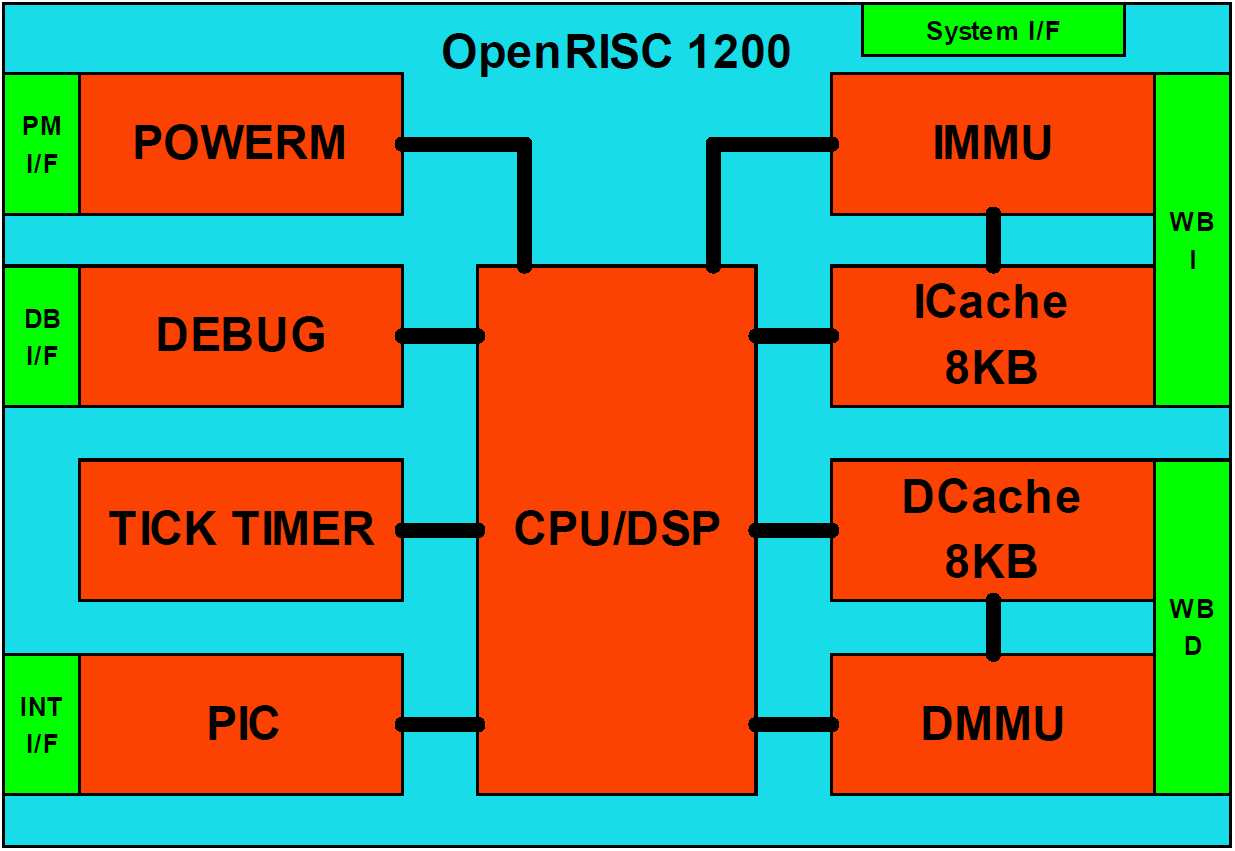
\includegraphics[scale=0.45]{openrs1200.png}
%	\caption{Bloková schéma procesora OpenRISC 1200.\cite{openrisc}}
%	\label{f:o_orisc}
%\end{figure*}

\begin{figure*}[h]
	\centering
	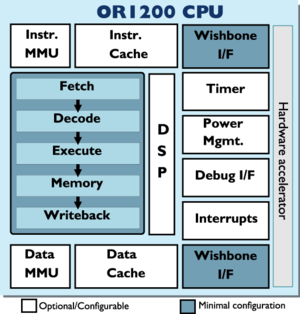
\includegraphics[scale=0.6]{a_Or1200.png}
	\caption{Bloková schéma procesora OpenRISC 1200.\cite{openrisc}}
	\label{f:o_orisc2}
\end{figure*}
%http://www.isy.liu.se/en/edu/kurs/TSEA44/OpenRISC/or1200_spec.pdf
%http://opencores.org/or1k/OR1200_OpenRISC_Processor
OpenRisc1200 procesor je implementácia rodiny procesorov s označením OpenRisc1000 a má nasledovné základné parametre:
\singlespacing
\begin{itemize}
\item 32 bitový RISC procesor,
\item 8 kB cache pamäť pre inštrukcie,
\item MMU s podporou pre virtuálnu pamäť,
\item 5 stupňový pipelining inštrukcie,
\item 3 hlavné módy regulácie spotreby,
\item podpora DSP,
\item centrálny CPU blok spolu s DSP,
\item IEEE 754 kompatibilná jednotka pre prácu s pohyblivou rádovou čiarkou (FPU Floating Point Unit),
\item priamo mapovaná dátová cache pamäť,
\item priamo mapovaná inštrukčná cache pamäť,
\item dátová MMU založená na hashovaní pre dátový TLB (Translation Lookaside Buffer),
\item inštrukčná MMU založený na hashovaní pre inštrukčný TLB,
\item jednotka pre riadenie spotreby,
\item tick timer pre presné meranie uplynutého času,
\item jednotka pre debugovanie a vývojové rozhranie,
\item jednotka prerušení,
\item rozhranie kompatibilné s inštrukciami a dátami so štandardom WISHBONE B3\footnote{\url{http://cdn.opencores.org/downloads/wbspec_b3.pdf}}.
\end{itemize}
\onehalfspacing

\subsubsection{VAULTSECURE} \label{s_sd_vault}
%http://www.insidesecure.com/Markets-solutions/Payment-and-Mobile-Banking/Embedded-Secure-Element-for-Mobile2
Je vyvíjaná spoločnosťou INSIDE Secure. Karta je vhodná pre vnorené aplikácie, použitie v mobilných telefónoch, tabletoch, počítačoch a systémoch typu M2M. 
Secure element je založený na zabezpečenej ARM architektúre s použitým jadrom s označením SC300, čo je 32 bitový ARMv7-Cortex M3 procesor s podporou Thumb-2 inštrukčnej sady, s nízkou spotrebou a s vysokým výkonom. Kartu je možné zakúpiť s rôznymi veľkostami pamätí pre program a dáta, v závislosti od aplikácie a od požiadaviek na navrhovaný systém. \footnote{\url{https://www.arm.com/products/processors/securcore/sc300.php}}
\begin{figure*}[h]
	\centering
	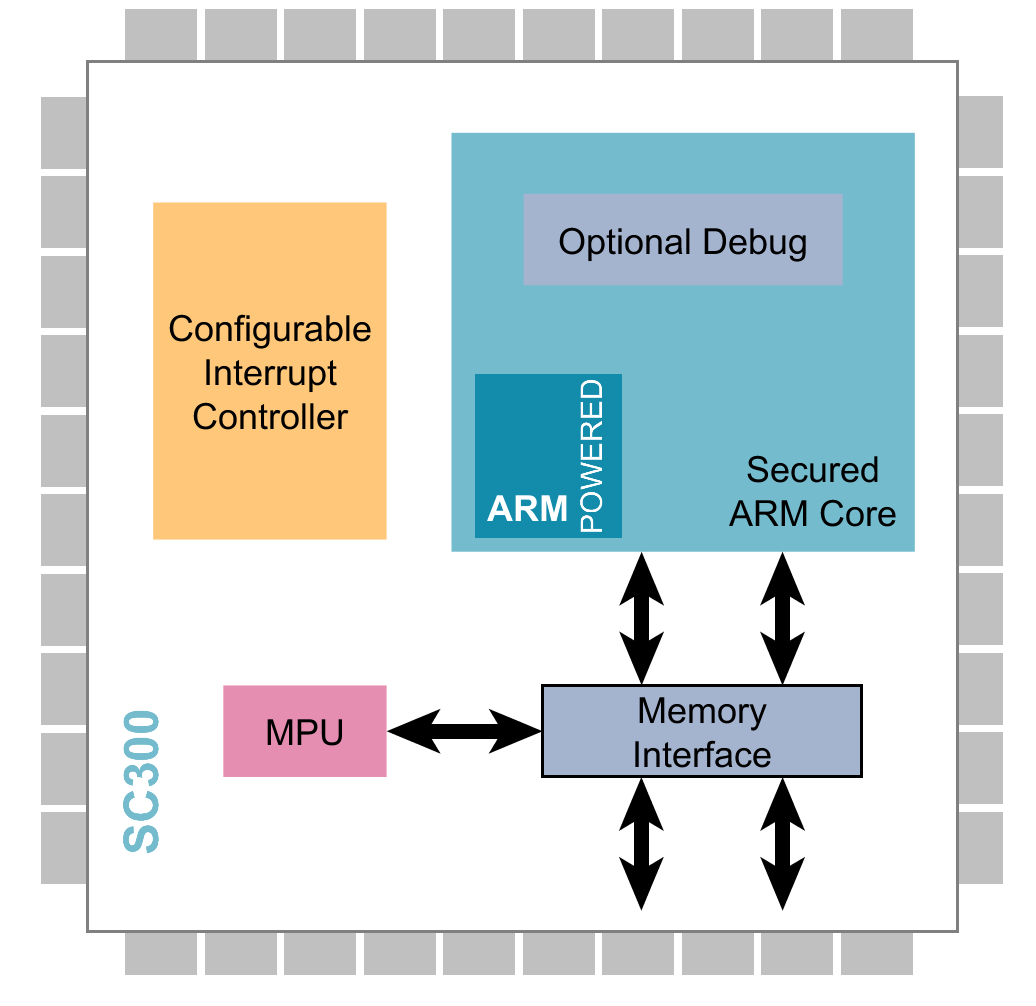
\includegraphics[scale=0.3]{a_sc300.png}
	\caption{Rodina ARM procesorov s označením SC300. \cite{sc300}}
	\label{f:o_sc300}
\end{figure*}
Výrobcovia udávajú nasledujúce parametre\cite{vaultsecure}:
\singlespacing
\begin{itemize}
\item Špecifikácia OS a kompatibilita:
\subitem JavaCard® 3.0.4 Classic Edition,
\subitem Global Platform® 2.2.1 dodatky A, C, D,
\subitem Global Platform® embedded SE Configuration compliant,
\subitem Global Platform® Requirement for embedded SE Interfaces compliant,
\item hardvérová špecifikácia:
\subitem 32-bitový RISC processor ARM SC300,
\subitem od 100 kB do 1 MB Flash pamäte,
\subitem do 24 kB RAM,
\item umožňuje komunikáciu prostrednícvtom protokolov:
\subitem SPI,
\subitem I2C,
\subitem ISO 7816,
\subitem SWP (Single Wire protocol),
\item poskytuje kryptografické funkcionality:
\subitem hardvérová realizácia algoritmov DES/3DES s ochranou proti DPA,
\subitem hardvérová realizácia algoritmu AES,
\subitem kompatibilný s MIFARE technológiou,
\subitem 32-bitový kryptografický akcelerátor pre algoritmy ako RSA, ECC, DH a ECDH,
\subitem CRC16 a CRC32,
\subitem kryptografické podpisovanie kódu.
\end{itemize}
\onehalfspacing

\subsubsection{MicroSD OneCard} \label{s_sd_usd}
%http://rdas.sk/
%http://www.nfcworld.com/2012/10/16/320548/logomotion-launches-nfc-microsd-card/
MicroSD karta s názvom OneCard je vyvíjaná spoločnosťou Logomotion\footnote{\url{http://www.smk-logomotion.com/}} v spolupráci so spoločnosťou RDAS s.r.o\footnote{\url{http://rdas.sk/}}.
%The Smart Card Controller hardware comprises of 8 bit processing unit, volatile and non-volatile memories accessible via a memory management unit, cryptographic co-processors, security components and three communication interfaces. 
Secure element je založený na procesore intelovskej rodiny x51 od spoločnosti NXP, ktorá bola založená spoločnosťou Philips. Procesor je rožšírený o sadu špecializovaných inštrukcií pre prácu s pridanými hardvérovými jednotkami.
SD karta obsahuje NFC anténu a obsahuje aj rozhranie štandardu ISO7816. Obsahuje hardvérový generátor náhodných čísiel, hardvérovú podporu pre PKI infraštruktúru, DES koprocesor a koprocesor pre kryptografický algoritmus AES a eliptické krivky. Karta je použiteľná pre rôzne aplikácie od úschovy kryptografických klúčov, v zdravotníctve, verejnej doprave, elektronických platbách, mobilných aplikáciach a im podobných.

%http://www.nfcworld.com/2012/10/16/320548/logomotion-launches-nfc-microsd-card/
\begin{figure*}[h]
	\centering
	
\includegraphics[scale=0.4]{logomotion-nfc-microsd.jpg}
	\caption{Logomotion MicroSD karta.\cite{lgmsd}}
	\label{f:usd}
\end{figure*}

\begin{figure*}[h]
	\centering
	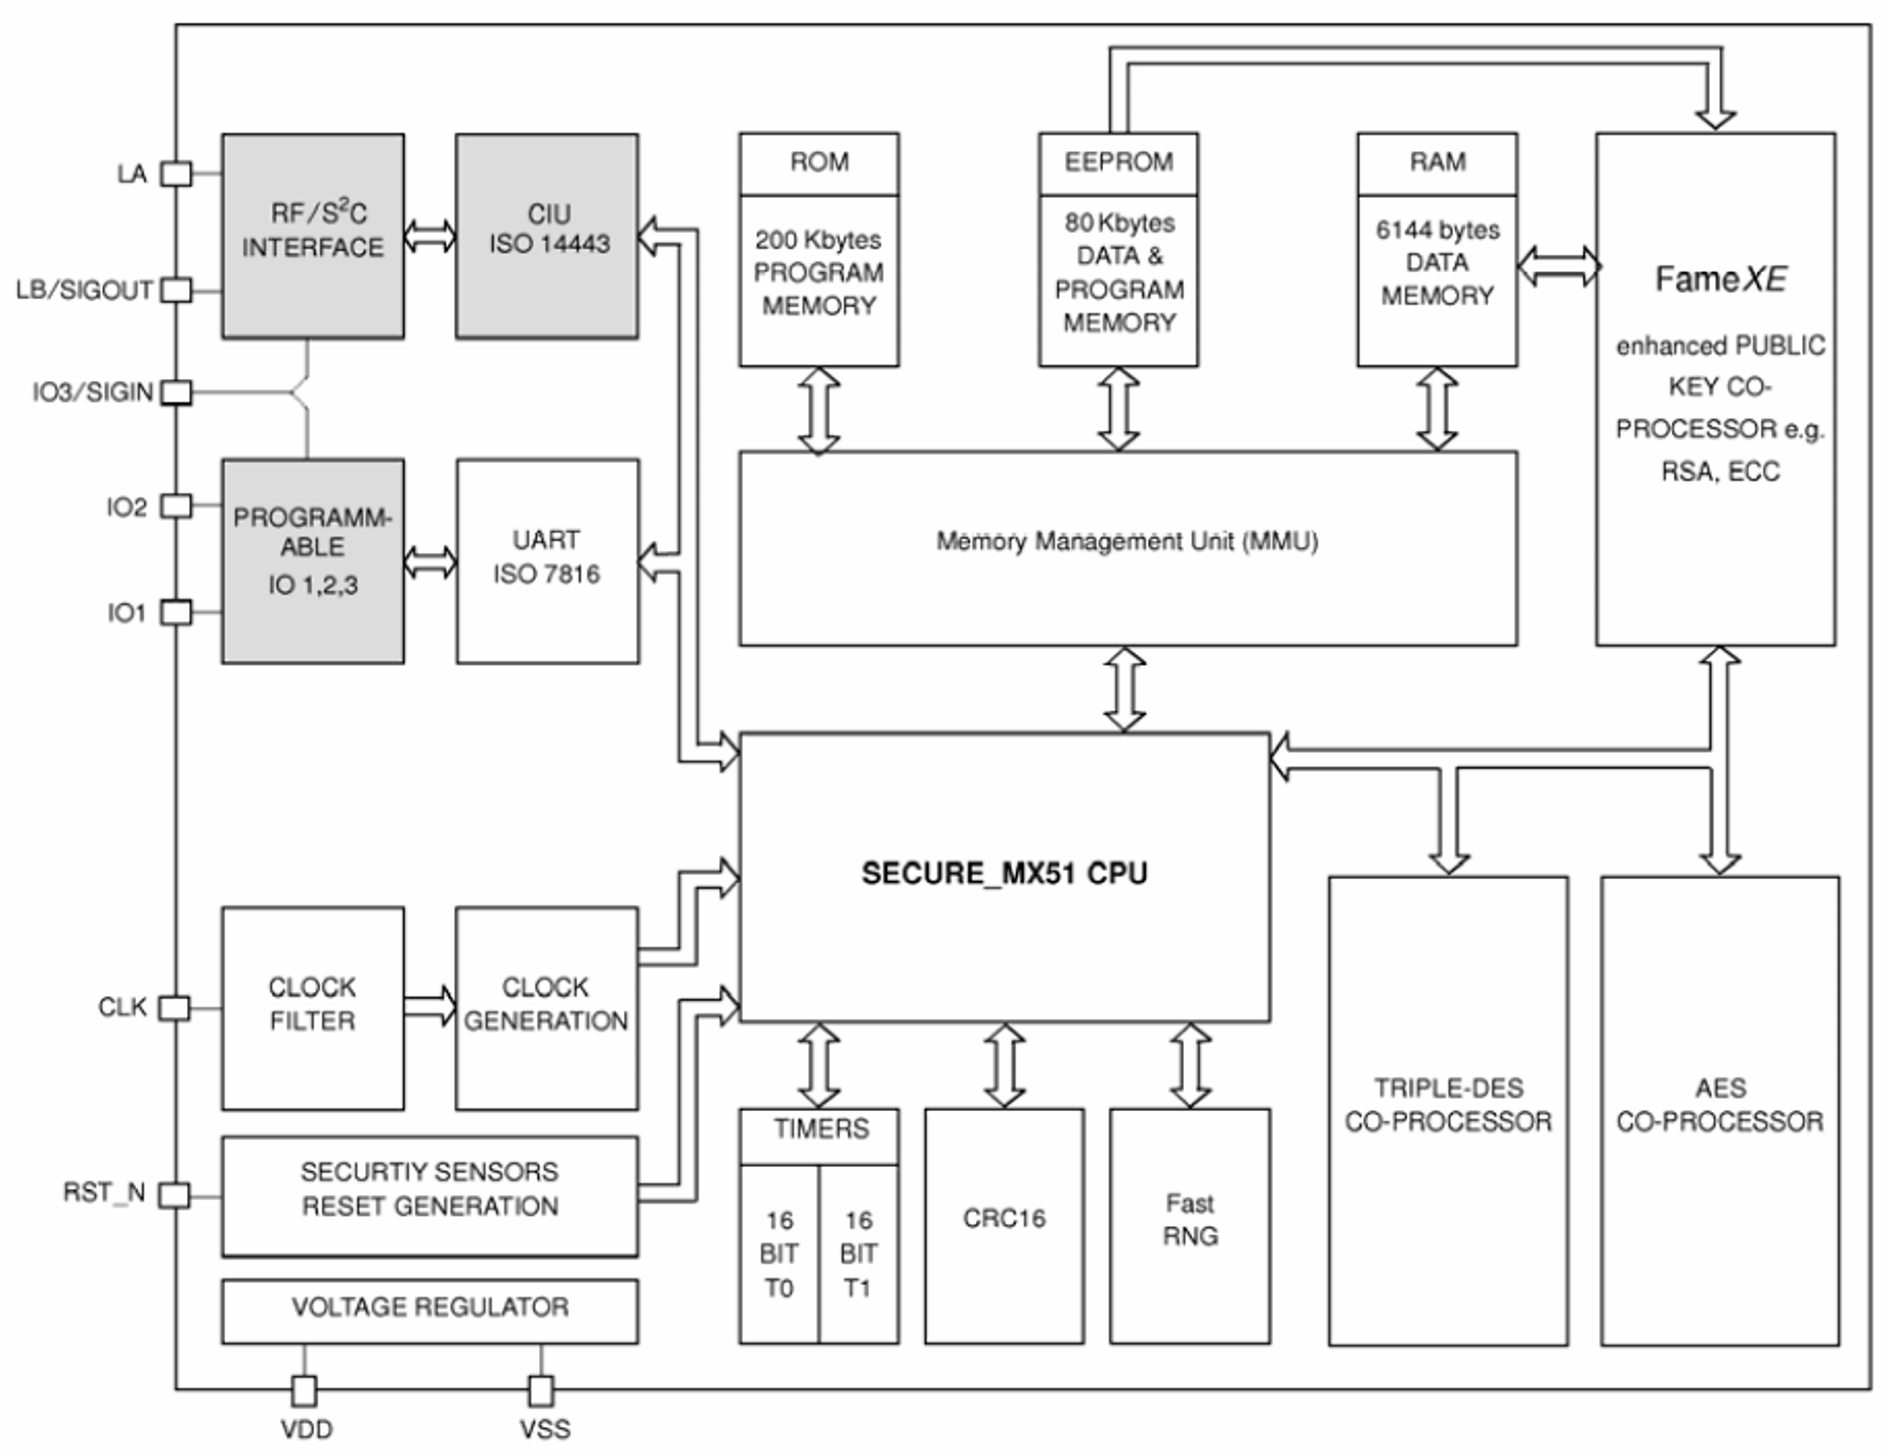
\includegraphics[scale=0.3]{s_analysis_usd1.png}
	\caption{Bloková schéma procesora x51 s rozšíreniami. \cite{nxpp5c}}
	\label{f:o_usd1}
\end{figure*}


\section{Porovnanie centralizovaných a decentralizovaných sietí} \label{s_centrilized_decentrilized}
%podla rozlohy LAN MAN WAN
%medium
%Synchornne
%asynchronne
%klient server
%Two-tier architectures
Podkapitola stručne porovnáva hlavné črty centralizovaných a decentralizovaných architektúr.
Čisto centralizované siete odoberajú hlavnú rozhodovaciu logiku z koncových uzlov a všetky výpočty a nároky prenášajú na centralizovaný uzol. Centralizovaný uzol, pokiaľ nie je dostatočne zabezpečený a zálohovaný, predstavuje potencionálnu hrozbu v podobe single-point-of-failure, ak zlyhá, tak zlyhá celá sieť napr. pri výskyte hardvérovej poruchy, sotvérovej poruchy alebo pri jeho kompromitácií. Preto voľbu čistého centralizovaného riadenia je potrebné vhodne zvážiť. Všetky dôležité informácie, rozhodovacie algoritmy sú však umiestnené v centralizovanom uzle.
Centralizovaná architektúra je jednoduchšia na odladenie jednotlivých funckionalít v porovnaní s decentralizovanou logikou. Výkon a limitácie celej siete závisia na výpočtovom výkone centrálneho uzla.

V decentralizovaných architektúrach sa každý prvok v sieti rozhoduje sám za seba v závislosti od vstupov a vnútorného stavu. Výpočtové nároky a nároky na samotný hardvér akými sú operačná pamäť, spotreba, pamäť pre program sú vyššie v porovnaní od centralizovaných architektúr, keďže každý uzol musí byť schopný udržiavať routovacie tabuľky, reagovať na vzniknuté situácie a byť robustný s pohľadu zabezpečenia. Pri zlyhaní jedného alebo viacerých uzlov v sieti sa pri správnom návrhu sieť vie zotaviť automaticky bez toho, aby si koncový používateľ vôbec niečo všimol. Distribúcia nových verzií softvéru na jednotlivé uzly je o kúsok zložitejšia ako preprogramovanie jedného centralizovaného uzla. Rekonfigurácia a manažovanie jednotlivých uzlov je v tomto prípade takisto náročnejšia.

%handbook of information and communicatiin security

%semicentralizovane
%centralizovane
%decentralizovane peer to peer 

\chapter{Návrh} \label{s_navrh}
Kapitola sa zaoberá návrhom dôležitých častí siete a prideľuje hlavné funkcionality jednotlivým systémom.

\section{Architektúra siete}
Základná navrhnutá bloková schéma architektúry je zobrazená na \ref{f:o_blok_topology}. Podrobnejšie rozkreslená bloková schéma je zobrazená na diagrame \ref{f:o_advanced_topology}.

Navrhovaná architektúra sa skladá z nasledujúcich základných prvkov:
\singlespacing
\begin{itemize}
	\item centralizovaná riadiaca jednotka,
	\item certifikačná autorita,
	\item koncové zariadenia,
	\item prvky vytvárajúce komunikačnú sieť.
\end{itemize}
\onehalfspacing
Dodatočné prvky siete zabezpečujúce prídavnú funkcionalitu:
\singlespacing
\begin{itemize}
	\item patria sem dedikované honeypot-ové zariadenia, ktoré by mali generovať náhodnú komunikácie s riadiacou jednotkou, ktoré budú vysielať na vyššom výkone ako ostatné koncové zariadenia a prípadné potencionálne hrozby budú hlásiť centralizovanému uzlu,
	\item ďalej sem patria špecializované uzly na detekciu kompromitovaných uzlov podľa\cite{compromisedsensors}. Ich implementácia do navrhovanej site nieje možná, keďže by na sieti obchádzali komunikáciu cez centralizovaný uzol a komunikovali by napriamo s ostatnými zariadeniami.
\end{itemize}
\onehalfspacing
%Zabezpecujeme proti jendoltivym utokom a jednotlive kroky ktore vedu ku kompormitacii a process utoku.

Každý prvok v sieti bude mať osadené zariadenie v podobe kryptovacieho elementu, poprípade . Tým sa zabezpečí, že každý prvok v sieti bude zabezpečený na rovnakej úrovni má rovnaké bezpečnostné možnosti, keďže reťaz je tak silná ako jej najslabší článok.

Kryptovanie od uzla k uzlu asi nieje nutné, keďže PKI infraštruktúra spolu s AES kryptovaním by mala poskytovať dostatočne bezpečné end-to-end šifrovanie s autentifikáciou.

Pre správne bezpečnostné zabezpečenie je nutné myslieť aj na zber dát v podobe auditných záznamov, samozrejme na prijateľnej úrovni v závislosti od použitých architektúr a možností hardvéru, napr. v podobe číselníkov, ktoré budú preddefinované, aby sa šetrilo miesto v pamäti a bola možná realizácia aj na menších 8-bitových architektúrach. Aby v prípade vzniku bezpečnostnej udalosti, bolo možné vykonať dostatočnú post-mortem analýzu stavu siete a jednotlivých uzlov v sieti. Na tento účel môže poslúžiť aj vnútorná zabezpečená pamäť microSD karty, ktorá nám zabezpečuje, že dáta nemôžu byť  modifikované ani manipulované bez patričných oprávnení. Pristúpiť k nim bude môcť iba autorizovaná osoba. Dáta by mali byť uchovávané spolu s časovou značkou. Pri preplnení pamäte sa môžu začať prepisovať najstaršie dáta.
Ilustračný príklad preddefinovaného číselníka:
%\singlespacing
\begin{itemize}
	\item 1: CRC chyba v prijatom pakete,
	\item 2: neplatný certifikát,
	\item 3: strata paketu, 
	\item 4: neprijaté ACK,
	\item 5: duplikovaná správa,
\end{itemize}
\onehalfspacing

Systém treba navrhnúť tak aby bol rozšíriteľný a bezpečný. Treba dbať aj na bezpečný návrh prislúchajúceho softvéru.
Jednotlivé uzly by mali byť odoloné proti istým SW alebo HW chybám a mohli by mať implementované ošetrenia na HW úrovni s možnosťou automatického zotavenia, napr. pomocou implementácie WatchDog časovača. Keďže niektoré koncové zariadenia môžu riadiť kritické a potencionálne nebezpečné zariadenia ako plynové kotle.

\subsection{Centralizovaná riadiaca jednotka} 
Jednotka je v prvom rade zodpovedná za zber dát zo vstupných senzorov, ich spracovanie, uloženie, kvôli štatistikám a riadení koncových uzlov. Prostredníctvom centralizovanej jednotky používateľ pristupuje k celému systému. Centralizovaná jednotka, ktorá by mala poskytovať nasledovné funkcionality:
%\singlespacing
\begin{itemize}
	\item plní funkciu brány, poskytuje konektivitu na internet, tzn. implentácia firewall-u niekde medzi centralizovanou jednotkou a internetom,
	\item monitorovanie stavu siete,
	\item manažment a konfiguráciu siete,
	\item evidenciu dovolených zariadení na sieti,
	\item evidenciu zakázaných zariadení na sieti,
	\item evidenciu aktívnych koncových uzloch na sieti,
	\item pridávanie a odoberanie prvkov siete,
	\item ohlasovanie identifkovaných neštandardných situácií, na základe vhodných metrík,
	\item ohlasovanie, ktoré koncové zariadenie potrebuje vymeniť batérie,
	\item mala by podporovať automatický režim riadenia vybraných systémov a manuálne nastavenie iných systémov,
	\item mala by byť jednoduchá na použitie,
	\item a netreba zabúdať ani na iné možnosti paralélneho prístupu k systému, či už pomocou mobilnej aplikácie, desktopovej aplikácie, poprípade ošetrených API služieb.
\end{itemize}
\onehalfspacing

%Netreba zabúdať, že dom môže byť viacpodlažný a zákazník môže žiadať inštaláciu viacerých terminálov. Tým pádom treba zabezpečiť distribúciu potrebných dát pre tieto terminály a treba riešiť aj prístup k zdieľaným prostriedkom. Ak by dvaja používatelia chceli nastavovať tie isté parametre. Jedno riešenie by bolo, tieto terminály integrovať do samotnej architektúry ako koncové zariadenia.
Návrh nerieši otázky rozmiestnenia, fyzického ani logického zabezpečenie hlavného centralizovaného uzla, zálohy databáz ani formát a štruktúru uložených dát ani politiky prístupu. Pri realizácií finálneho produktu treba myslieť na dostatočné zabezpečenie tohto uzla, keďže na ňom závisí celé riešenie.
Otázku, ako sa dostanú dáta z jedného koncového uzla do druhého, ak druhý uzol potrebuje jeho dáta, je ponechaný na centralizovanú riadiacu jednotku, ktorý má prehľad o aktuálne pripojených koncových zariadeniach.

\subsection{Certifikačná autorita}
Vlastná certifikačná autorita zabezpečuje overenie pravosti páru kľúčov pri ich generovaní, programovanie kľúčov do secure elementov, evidenciu používaných a vyradených klúčov, generovanie a podpisovanie certifikátov pre jednotlivé uzly.

\subsection{Koncové zariadenia} 
Pri návrhu treba brať do úvahy podporu zhlukovania koncových zariadení alebo zariadení tvoriacich sieť do logicky súvisiacich blokov a ich spoločné riadenie, poprípade manažovanie. Napr. na základe rozmiestnenia po miestnostiach, alebo podľa typu uzla. Ponúkajú sa dve riešenia. Rozlišovať zariadenia na vyšších aplikačných vrstvách pomocou algoritmov, alebo logicky závislé prvky budú rozmiestné na sieťach z rôznym identifikátorov siete. Smerovanie by prebiehalo medzi rôznymi sieťami a broadcast na danej sieti by sa prešíril iba zainteresovaným koncovým zariadeniam.
Treba sa rozhnodúť, či koncové zariadenia môžu obsahovať malú lokálnu logiku. Napr. v prípade zlyhania centralizovaného uzla, aby mohol používateľ systému v prípade núdze otvoriť dvere ovládané pomocou systému na základe identifikácie napr. pomocou NFC rozhrania na microSD karte.
V prípade neštandardných situácií, sa treba zamyslieť nad automatickým ohlasovaním vzniknutých udalostí od koncových uzlov centralizovanej riadiacej jednotke.
% Treba však zvoliť vhodnú implementáciu s obmedzeniami, aby neprišlo k samovoľnému preťaženiu siete a jednotlivých uzlov.

\subsection{Prvky sieťovej architektúry}
%V závislosti od veľkosti siete, počtu zariadení a požadovaných prevádzkových parametrov siete bude treba vybrať z dostupných možných topológií ZigBee protokolu.
Primárna funkcia je vytvoriť prepojenú komunikačnú sieť medzi koncovými zariadeniami a centralizovanou riadiacou jednotkou.

%Navrhuta architektura siete
Zabezpečenie jednotlivých bezpečnostných cieľov pomocou bezpečnostných mechanizmov:
\singlespacing
\begin{itemize}
	\item autorizácia: certifikáty a PKI,
	\item autenticita správy: PKI a CRC,
	\item nepopieratelnosť prijatia: potvrdzovanie správ o ich prijatí,
	\item integrita správ: digitálne podpisovanie dokumentov a CRC,
	\item zabezpečenie proti retransmission a duplicite: počítadlom paketov,
	\item eskalovanie privilégií a zabezpečenie proti sidechannel analýze: kritická logika vie byť implementovaná vo forme appletu na secure elemente.
\end{itemize}
\onehalfspacing
%dostupnost
%confidentiality
%gaining access
%proti analyze beziacich sluzieb a procesov

%Záložná logická adresa, v pripade zahltenia alebo zlyhania

%Ci budu uzly na alebo sa topológia bude obmienat po pripojeni tychto uzlov
\section{Formát posielaných dát}
Navrhovaný formát dát je orientovaný na čo najefektívnejšie využitie prenosového pásma. 
Pre zabezpečenie lepšej čitateľnosti a rozšíriteľnosti v budúcnosti, dáta by sa mohli posielať v ľudsky čitateľných formátoch ako JSON alebo XML.
% Dáta a formát paketu je zatiaľ navrhovaný tak, aby sa všetky potrebné informácie, ktoré sa majú preniesť, zmestili do jedného paketu.

%Ponúka sa otázka, či chceme mať implementované aj metódy proti reverznému inžinierstvu, na základe deterministických pravidiel, rotovaním dát po bitoch pred zakryptovaním, ktoré sú následne posielané v z Zigbee pakete. Ďalšia z ponúkaných metód je dopĺnať nevyužité miesto v pakete o padding náhodnej dĺžky, ktorý bude obsahovať náhodne vygenerované dáta.
Posielané dáta budú kryptované pomocou štandardu AES-128 s využitím. Dáta tak budú kryptované dvojúrovňovo.

%ci to chceme zmestit do jedneho, alebo viacerych. Do jedneho, kvoli vypoctovej narocnosti a problemami ak nieco pokazi na niektorej strane, cislovanie jednotlichv paketov
%Spominany zigbee packet, jeho v kapitole ZigBee.
Navrhované dáta sú zabalené v pakete pre príslušný komunikačný protokol:
% tak aby sa zmestili do 127 B
\singlespacing
\begin{itemize}
	\item certifikát zariadenia,
%	\item magic number,
	\item ID cieľového zariadenia alebo služby,
	\item CommandID: identifikácia príkazu, ktorý sa má vykonať, zhasnúť svetlá, stlmiť osvetlenie, nastaviť farbu a pod.
	\item GroupID: identifikácia cieľovej skupiny zariadení,
	\item Configuration: príznak hovoriaci či sa jedná o konfiguráciu cieľového zariadenia,
	\item GetStatus, SetStatus: identifikátor žiadosti o dáta alebo o spracovanie dát,
	\item stream, priority: identifikátor priority dát alebo identifikátor streamovaných dát malých objemov,
	\item reserved: miesto vyhradené pre zmeny v budúcnosti,
	\item payload: samotné dáta.
\end{itemize}
\onehalfspacing

%logical network id 0 -2\textsuperscript{16}-1 255 255 vsetky.
%Návrh štruktúry posielaných dát.

\section{Formát cerifikátu}
Aby sme zamedzili útoku Man in the Middle, je nutné používať a implementovať zabezpečenie pomocou  certifikátov. Certifikáty sú generované a distribuované ešte pred nasadením koncového zariadenia do siete, napr. cez komunikačné rozhranie NFC s vlastnou certifikačnou autoritou. Certifikačná autorita pošle koncovému zariadeniu aj vlastný certifikát, aby si ho mohlo zariadenie počas prevádzky porovnať, či naozaj komunikuje s certifikačnou autoritou.
 Pre efektívne využitie prenosového pásma, samotný certifikát bude obsahovať iba najnutnejšie položky. Výmena certifikátu za nový, bude prebiehať použitím zabezpečenej komunikácie, prostredníctvom existujúcej siete. Certifikačná autorita vygeneruje nový certifikát. Ten sa následne na pošle cez komunikačnú sieť koncovému zariadeniu a po úspešnej verifikácií si ho uloží do zabezpečeného úložiska.

% (CRC check a verifikácia digitálneho podpisu)

\begin{figure*}[h]
	\centering
	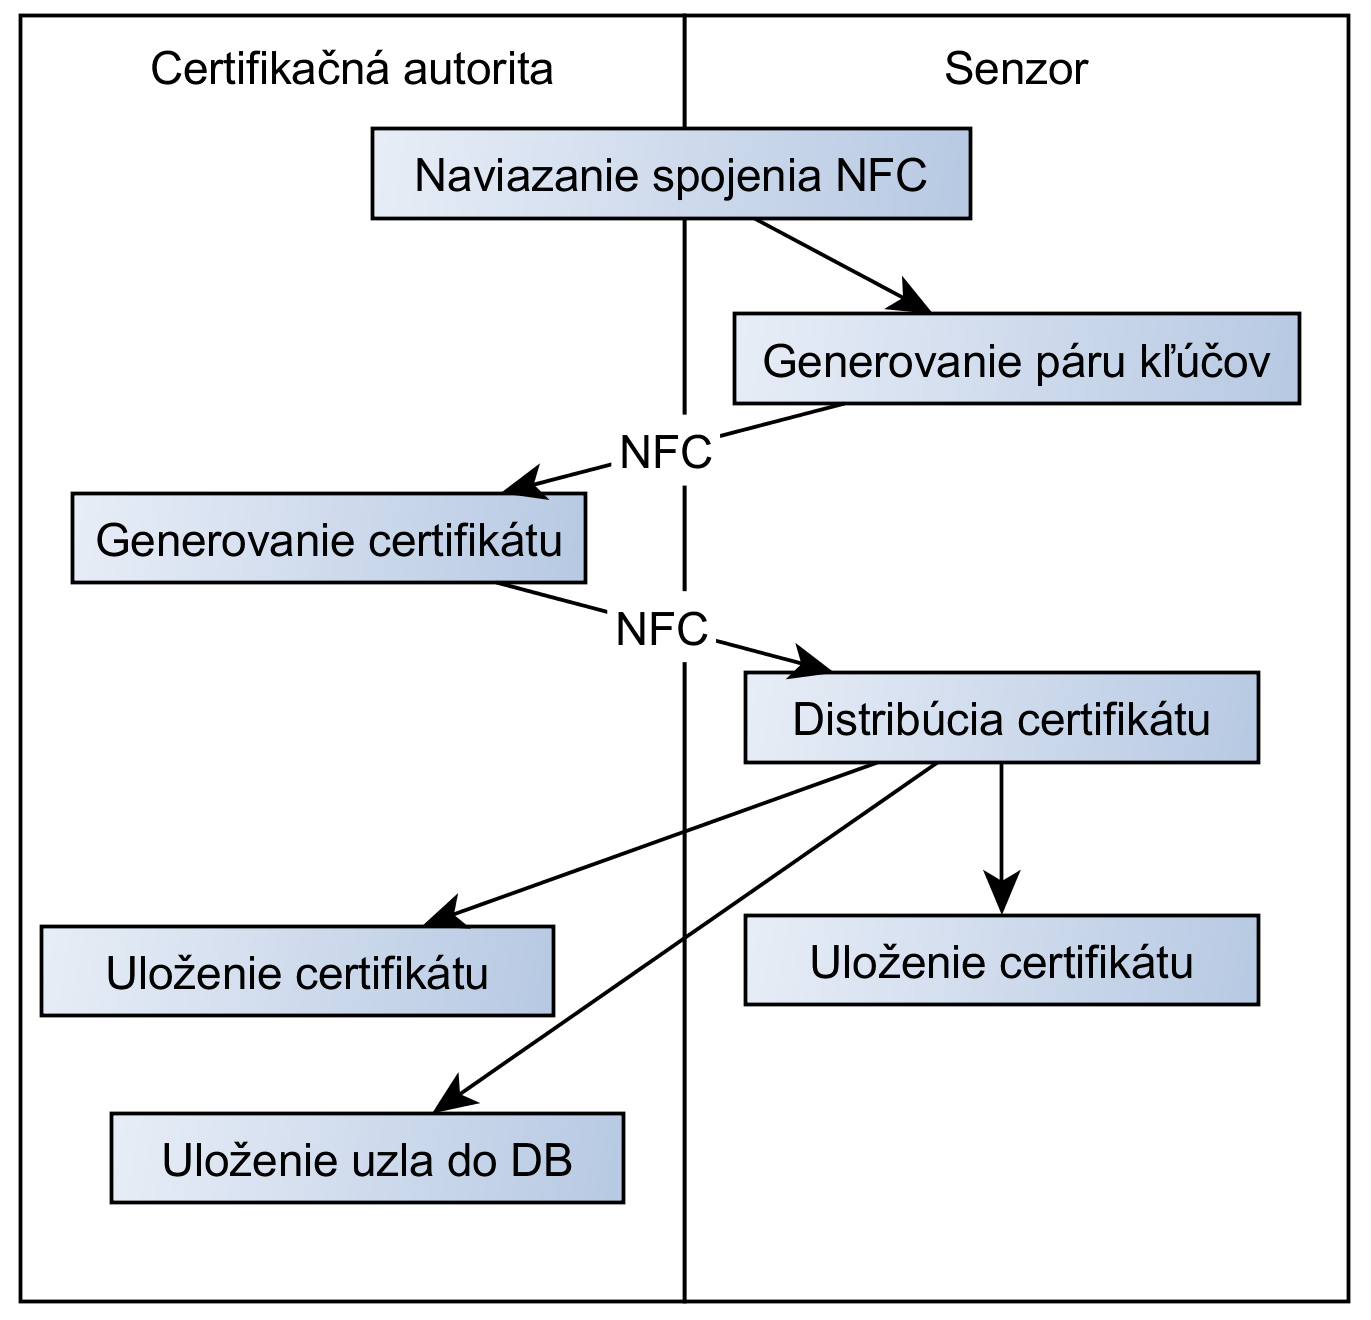
\includegraphics[width=8cm]{n_precondition.png}
	\caption{Prvotné vygenerovanie a rozdistribuovanie certifikátov.}
	\label{f:n_CA_distribution}
\end{figure*}


Identifikované základné a potrebné parametre  certifikátu:
%\singlespacing
\begin{itemize}
	\item Identifikátor zariadenia,
	\item verejný kľúč zariadenia,
	\item typ uzla, či sa jedná o vstupné alebo výstupné zariadenie.
	\item elektronický podpis certifikačnou autoritou.
\end{itemize}
\onehalfspacing

\section{Konvergencia siete}
Po zapnutí napájania sa vykoná jednoduchý Power on Self test, ktorý otestuje relevané funkcionality alebo pripojené hardvérové komponenty jedtnotlivých zariadení. Po úspešnom vykonaní testu si všetky uzly nastavia time-out na náhodnú hodnotu. Po uplynutí tohto časového limitu si uzol vyžiada, na ktorej logickej adrese sa nachádza centralizovaná riadiaca jednotka s certifikačnou autoritou napr. pomocou broadcastu. Riadiaca jednotka pošle svoj certifikát a zakryptuje aktuálny čas svojim privátnym klúčom. Vykoná sa autentifikácia od koncového uzla smerom k centralizovanej riadiacej jednotke. Koncové zariadenie pošle certifikát zakryptovaný certifikačnou autoritou. Tým koncové zariadenie vie, kde sa nachádza riadiaca jednotka a riadiaca jednotka má priradenú dvojcu (Logická adresa, Fyzické ID koncového zariadenia). Riadiaca jednotka si nastaví príznak, kedy a kde naposledy videla dané koncové zariadenie.

\begin{figure*}[h]
	\centering
	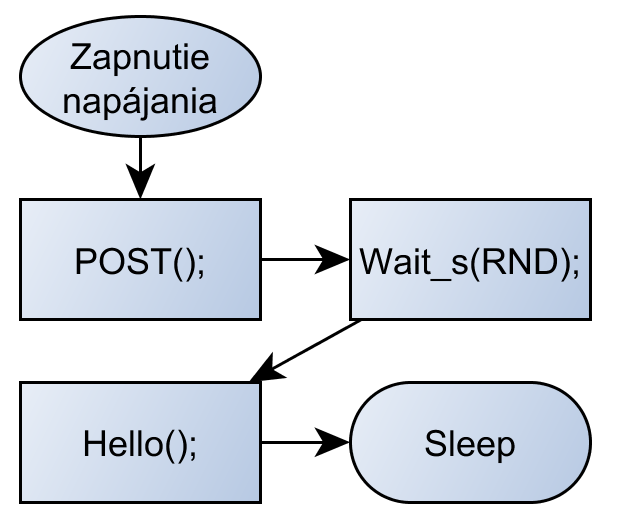
\includegraphics[scale=0.3]{n_konvergencia.png}
	\caption{Reakcia koncového uzla na udalosť.}
	\label{f:n_konvergenica}
\end{figure*}

Zariadenia sa budú v preddefinovaných pravidelných intervaloch hlásiť centralizovanému uzlu, že sú stále nažive. V prípade že uzol dlhšie neodpovedá, po prekročení nastavenej hraničnej hodnoty, môže centralizovaný uzol notifikovať používateľa o prípadnom probléme.

%\section{Architektúra}
%x
%https://webstore.iec.ch/preview/info_isoiec27039%7Bed1.0%7Den.pdf
%iso/iec 27039
%iso/iec 27034
Zišlo by sa zamyslieť nad implementáciou bezpečnostých mechanizmov na základe už existujúcich zadefinovaných smerníc a usmernení vytvorených odborníkmi v jednotlivých oblastiach a inšpirovať sa nimi. Medzi ne patrí napr. certifikačná a štandardizačná autorita ISO/IEC, konkrétne smernica 27039:2015, zaoberajúca sa kybernetickou a informačnou bezpečnosťou s názvom Security techniques Selection, deployment and operations of intrusion detection and prevention systems (IDPS)\cite{iso27039}, ktorá má zadefinovaný nasledujúci obsah:
\begin{itemize}
\item Integrita súborov a správ zabezpečená pomocou CRC a PKI,
\item firewall,
\item honeypot-y,
\item nástroje pre manažovanie siete,
\item nástroje pre Security Information Event Management (SIEM),
\item nástroje pre ochranu obsahu pred vírusmi,
\item nástroje na posúdenie zraniteľností,
\item ošetrenie výstrah,
\item odpovede na vzniknuté výstrahy,
\subitem aktívne: spustia sa preddefinovaé procesy, programy alebo spustí sa automatická hĺbková analýza siete, zariadenia prestanú vysielať, zmažú sa vybrané citlivé dáta.
\subitem pasívne.
\end{itemize}
\onehalfspacing

%iso/iec 27034 application security, to sa nas momentalne netyka v sieti

\begin{figure*}[h]
	\centering
	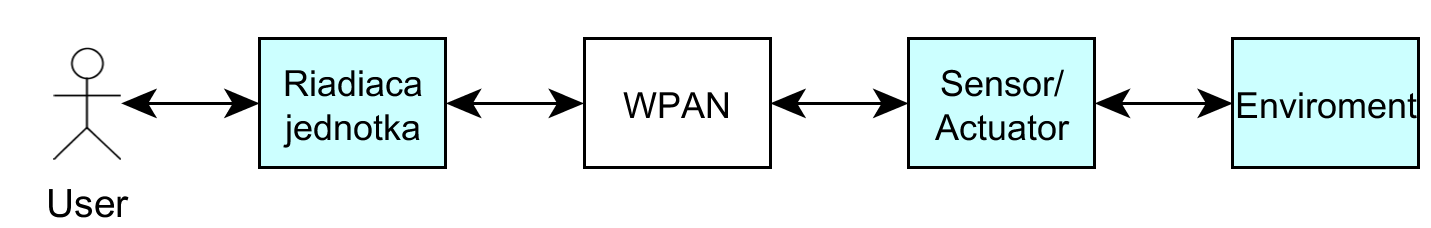
\includegraphics[scale=0.4]{n_topology.png}
	\caption{Jednoduchá bloková schéma siete.}
	\label{f:o_blok_topology}
\end{figure*}

\begin{figure*}[h]
	\centering
	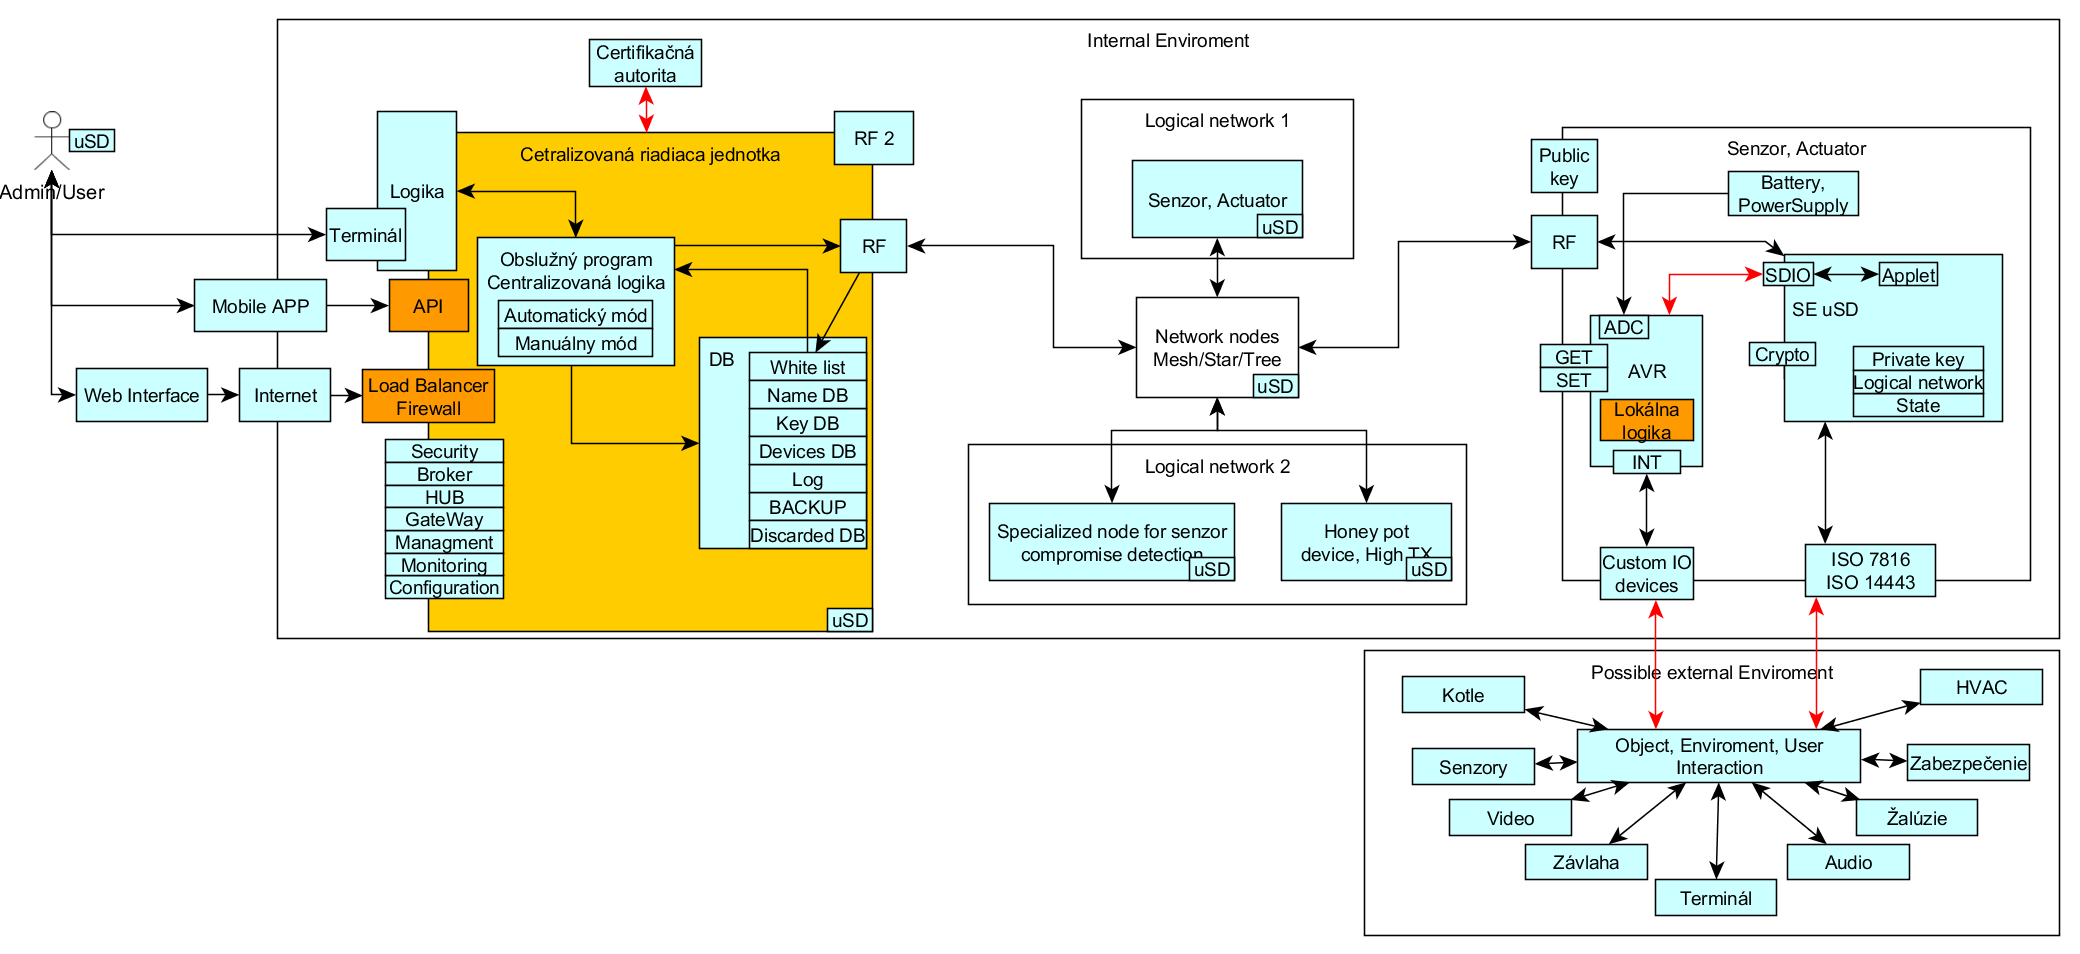
\includegraphics[width=20cm, angle=90]{n_topology0.png}
	\caption{Podrobnejšia bloková schéma navrhovanej topológie. Odtiene červenej farby predstavujú bezpečnostné riziká.}
	\label{f:o_advanced_topology}
\end{figure*}

\begin{figure*}[h]
	\centering
	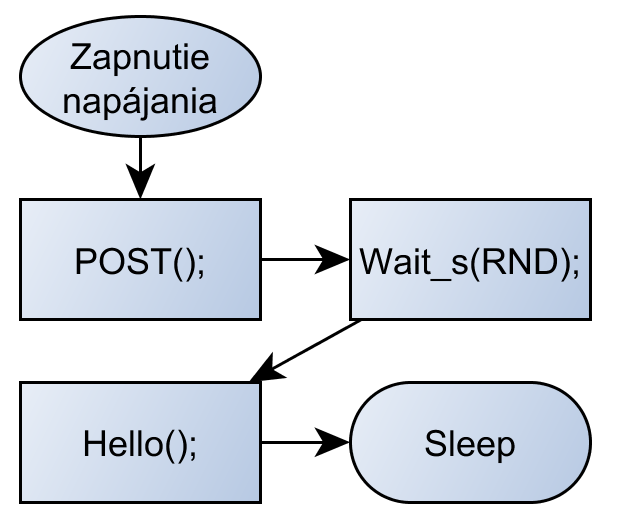
\includegraphics[scale=0.3]{n_konvergencia.png}
	\caption{Správanie sa koncového uzla po zapnutí napájania.}
	\label{f:o_konvergencia}
\end{figure*}

\begin{figure*}[h]
	\centering
	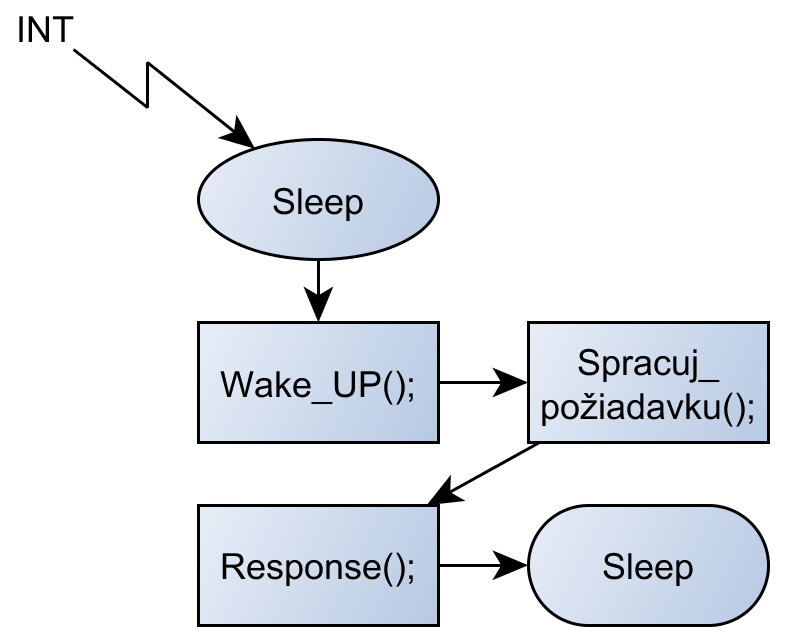
\includegraphics[scale=0.3]{n_event.png}
	\caption{Reakcia koncového uzla na udalosť.}
	\label{f:o_event}
\end{figure*}



\chapter{Implementácia} \label{s_implementation}
%\section{}
Za účelom overenia navrhnutého riešenia, boli vybraté zariadenia a protokoly opísané v tejto kapitole. Teoreticky nezáleží na zariadení, jeho architektúre ani na použitom komunikačnom protokole. Najdôležitejším cieľom použitých zariadení je získať kvantitatívne výsledky potrebné pre celkové vyhodnotenie návrhu a samotného projektu.

Overenie zabezpečenia komunikačnej sieti prebieha nad zmenšeným zjednodušeným modelom navrhnutej siete tvoreným iba z dvoch uzlov v sieti. Vybrané komunikačné moduly sa zaraďujú do produkčnej rady s označením nRF51 od firmy Nordic Semiconductor. Vývojový kit má osadený Arm Cortex-M0 mikroprocesor s označením nRF51422-QFAAC. Bloková schéma procesora je zobrazená na obrázku \ref{f:o_i_nrf51blockdiagram}. Základné vybrané parametre ktorými sa procesor vyznačuje sú\cite{nRF51}:
\begin{itemize}
	\item ARM Cortex-M0 32 bitový procesor,
	\item Thumb-2 inštrukčná sada,
	\item 3 úrovňový pipelining,
	\item 2.4 GHz vysielač v pásme ISM v rozmedzí frekvencií 2.4 - 2.4835 GHz s GFSK moduláciou a podporou protokolov napr. ANT alebo Bluetooth low energy,
	\item 256 kB pamäte pre program,
	\item 16 kB pamäte typu RAM,
	\item 16 MHz kryštál,
	\item 31 GPIO pinov,
	\item AES HW kryptovanie,
	\item Quadrature dekóder,
	\item UART,
	\item SPI rozhranie Master/Slave,
	\item Two-wire rozhranie kompatibilné s protokolom I2C,
	\item senzor teploty.
\end{itemize}
\onehalfspacing

\begin{figure*}[h]
	\centering
	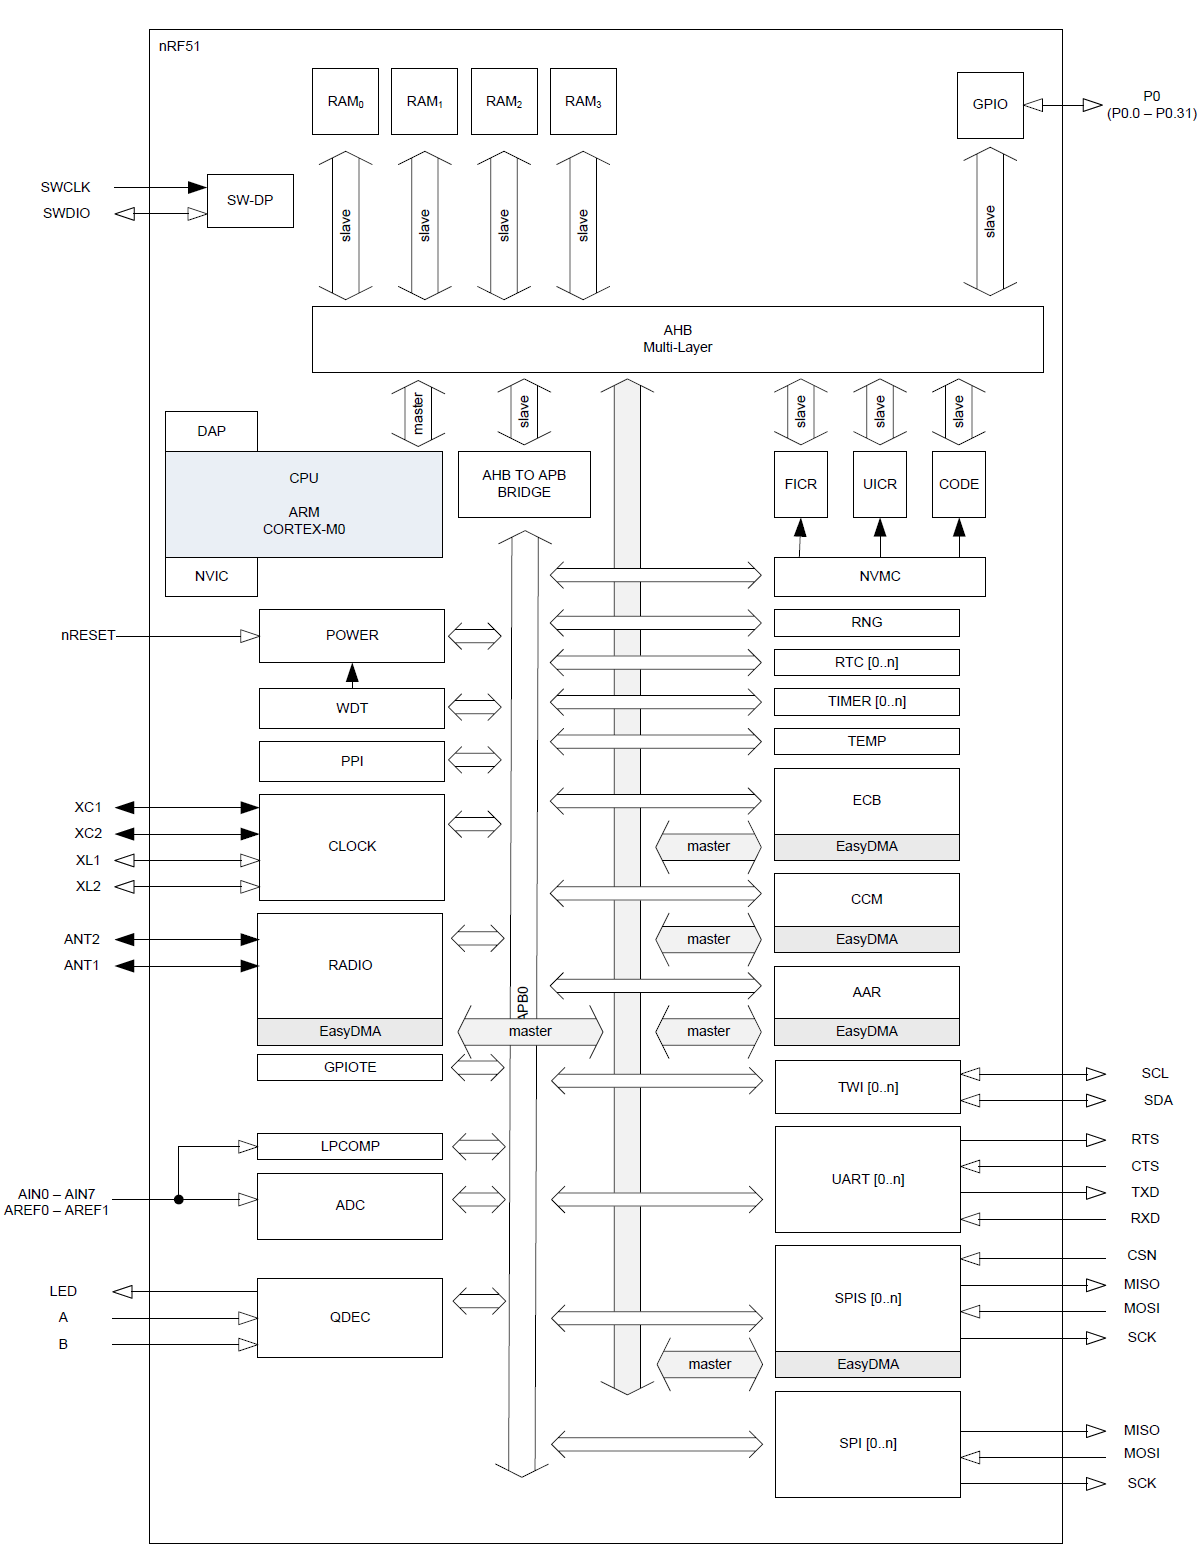
\includegraphics[scale=0.3]{i_nrf51blockdiagram.png}
	\caption{Bloková schéma procesora rady nRF51\cite{nRF51}.}
	\label{f:o_i_nrf51blockdiagram}
\end{figure*}

Konkrétne sa jedná o komunikačné moduly s označením PCA10006 a PCA10007. Obidve vývojové dosky sú osadené totožným, vyššie spomenutým procesorom rodiny ARM. Jediný rozdiel medzi doskami je vo vyvedenom externom koaxiálnom konektore, pre pripojenie antény na vývojovom kite PCA10007.
Komunikačné moduly majú natvrdo naprogramovaný neprepisovateľný SoftDevice S210 verzie 2.0.0. SoftDevice je označenie pre predkompilovaný a zlinkovaný protokolový zásobník. Použitý SoftDevice vo výsledku určuje, na akom protokole zariadenie funguje a môže komunikovať. Protokolový zásobník S210.2.0.0 potrebuje pre správne fungovanie 2 kB pamäte RAM a zaberá prvých 40 kB pamäte pre program. Vypočítané hodnoty, od ktorých môžeme umiestniť používateľský aplikačný program a dáta spolu s ich veľkostami, sú uvedené v tabuľke \ref{t:s210_memory}. Bloková schéma protokolového zásobníka v kontexte s okolím je na obrázku \ref{f:o_SD210}.

\begin{figure*}[h]
	\centering
	\includegraphics[scale=0.05]{i_siet.jpg}
	\caption{Zariadenia tvoriace zjednodušený model siete.}
	\label{f:i_devices}
\end{figure*}

ANT protokolový zásobník verzie 2.0 podporuje funkcionality\cite{SD210}:
\begin{itemize}
	\item rôzne typy topológií P2P, star, tree,
	\item nezávislosť na RTOS systémoch,
	\item bezpečné viacniťové softvérové rozhranie,
	\item asynchrónne, udalosťami riadené vykonávanie,
	\item kryptovanie jedného komunikačného kanála pomocou AES-128,
	\item asynchrónne posielanie dát,
	\item spravovanie až 8 rôznych sieťových kľúčov, pre komunikáciu na rôznych sieťach.
\end{itemize}
\onehalfspacing

CMSIS\footnote{\url{https://www.arm.com/products/processors/cortex-m/cortex-microcontroller-software-interface-standard.php}} (Cortex Microcontroller Software Interface Standard) je štandard navrhnutý spoločnosťou ARM za účelom zjednodušenia a urýchlenia vývoja softvéru na procesoroch rodiny ARM Cortex. Tento štandard sa skladá z viacerých spolu kompatibilných projektov, ktoré zabezpečujú podporu od RTOS, rozhranie pre ladenie a krokovanie programu, až po abstrakciu hardvéru a tým pádom istú nezávislosť a prenositeľnosť kódu od použitého hardvéru\cite{CMSIS}.

\begin{table}[h]
	\centering
	\caption{Začiatky spolu s veľkosťami jednotlivých pamäťových blokov pre program a dáta.}
	\label{t:s210_memory}
	\begin{tabular}{|c|c|c|c|}
		\hline
		\multicolumn{2}{|c|}{ROM} & \multicolumn{2}{c|}{RAM} \\ \hline
		Začiatok     & Veľkosť    & Začiatok     & Veľkosť   \\ \hline
		0xA000       & 0x36000    & 0x20000900   & 0x3700    \\ \hline
	\end{tabular}
\end{table}

\begin{figure*}[h]
	\centering
	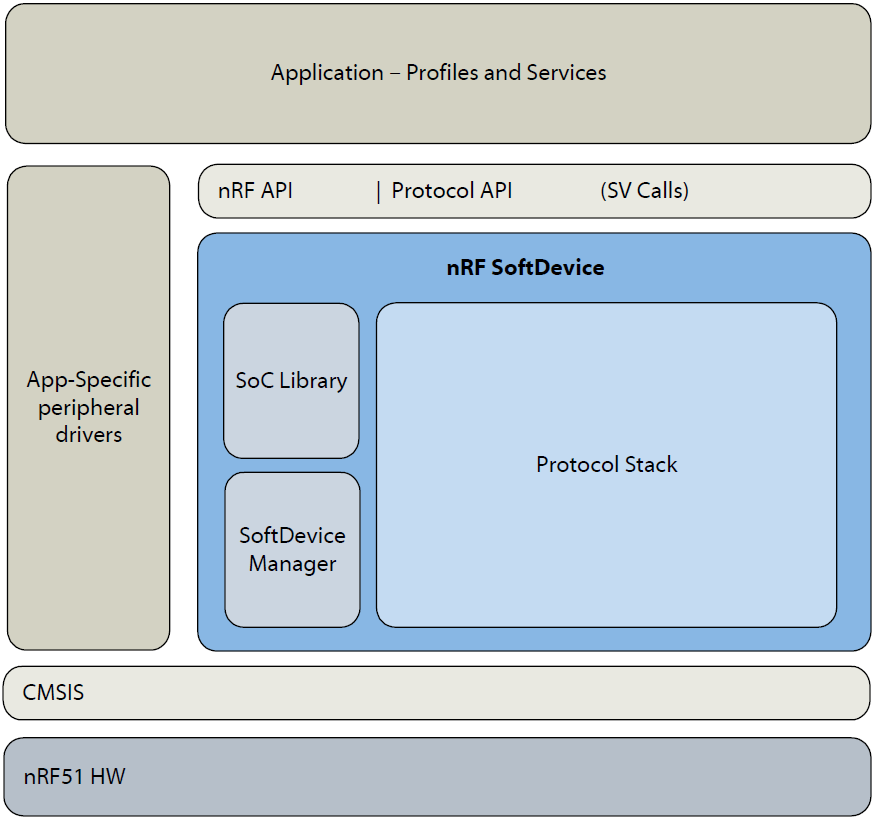
\includegraphics[scale=0.3]{i_SD210.png}
	\caption{Kompozícia SoftDevice-u v kontexte so zbytkom systému\cite{SD210}.}
	\label{f:o_SD210}
\end{figure*}

\begin{figure*}[h]
	\centering
	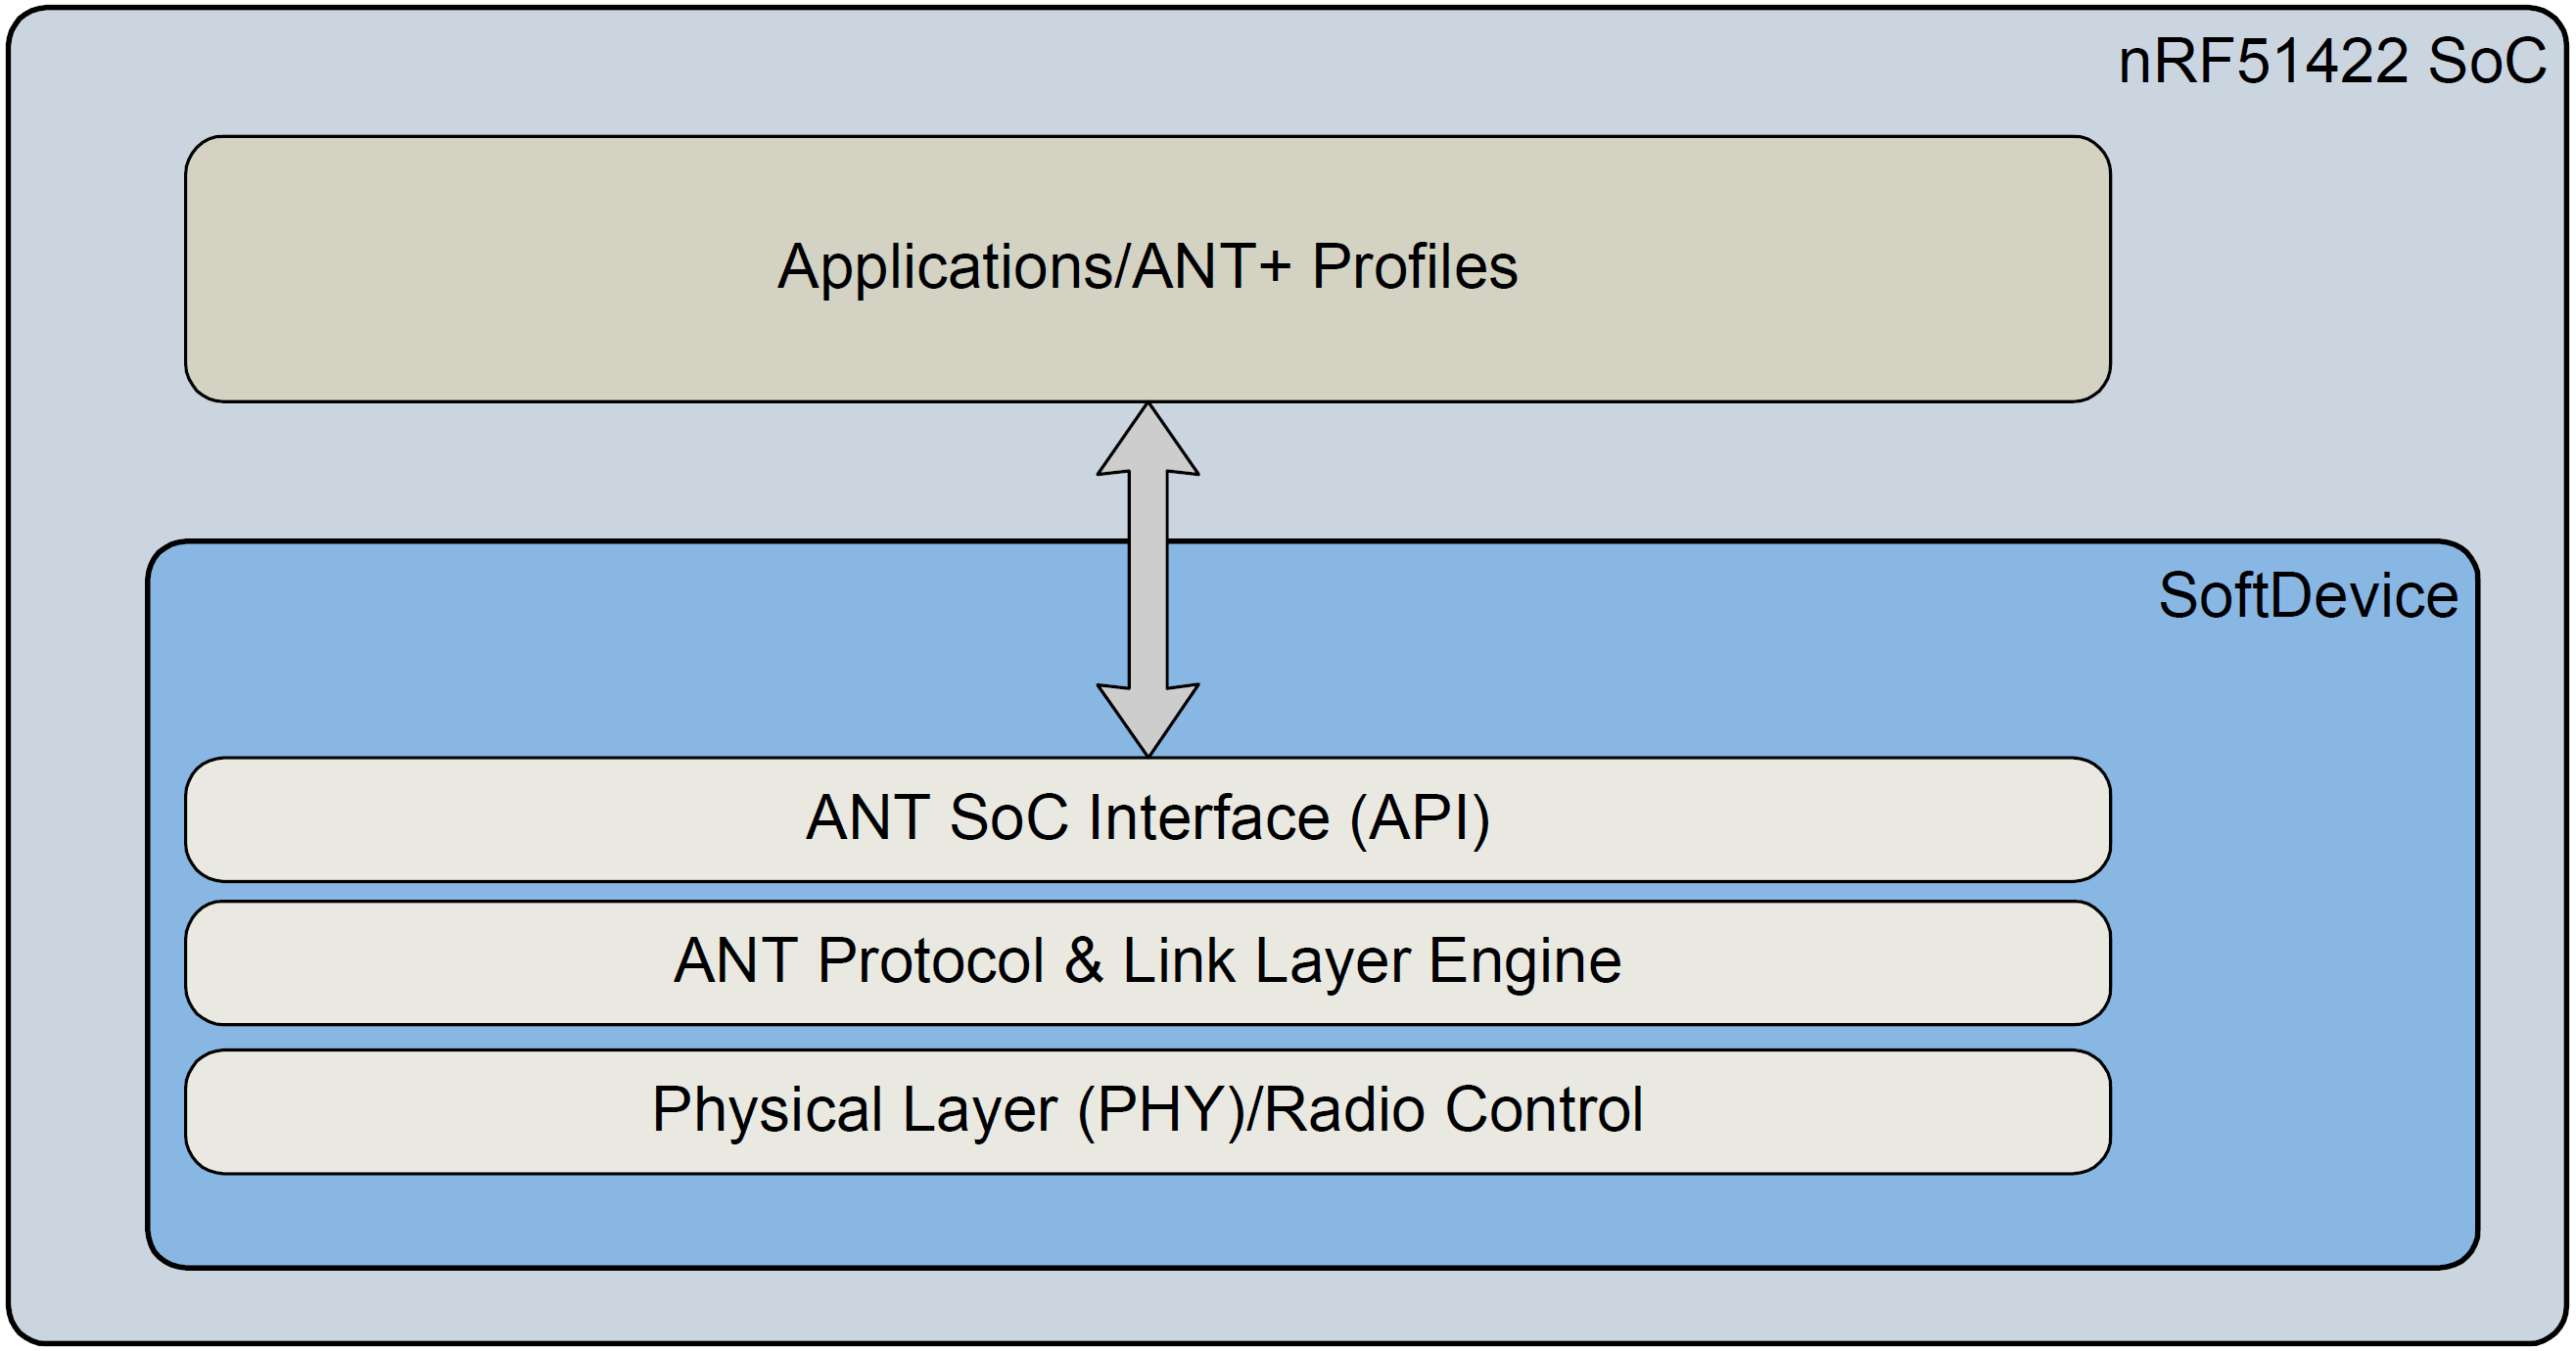
\includegraphics[scale=0.1]{i_SD210_nrf51422.png}
	\caption{Kompozícia a štruktúra protokolového zásobníka\cite{SD210}.}
	\label{f:o_SD210_alone}
\end{figure*}

\begin{figure*}[h]
	\centering
	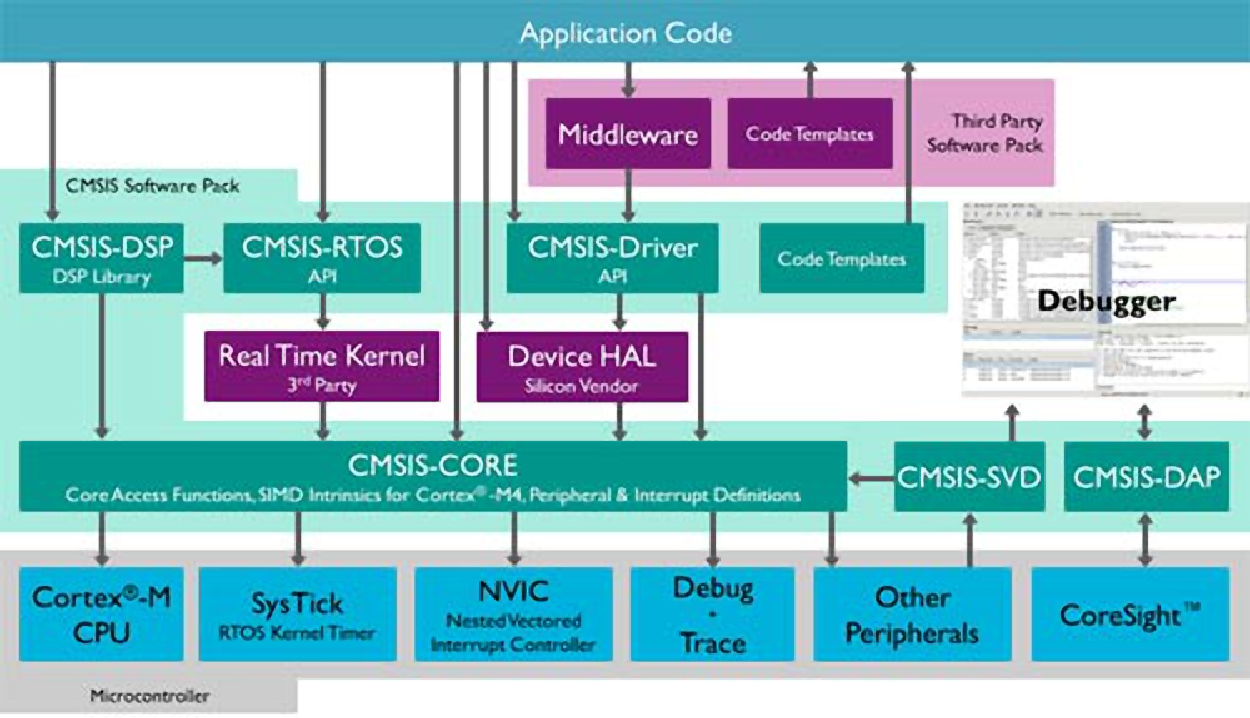
\includegraphics[scale=0.3]{i_CMSISv4_small.png}
	\caption{CMSIS infraštruktúra\cite{CMSIS}.}
	\label{f:o_CMSIS}
\end{figure*}
Pre účely zjednodušenia testovania je jeden z komunikačných modulov osadený na základovej doske od Nordic Semiconductor s názvom nRF6310 rev 1.3.
Vývoj kódu pre komunikačné moduly prebieha vo vývojovom prostredí Keil {\textmu}Vision verzie V5.21.1.0 v programovacom jazyku C. Pre vývoj kódu procesorov rodiny ARM je použitý MDK-Lite toolchain\footnote{\url{http://www2.keil.com/mdk5/editions/lite/}}. 
Programovanie a real-time debugovanie prebieha pomocou programátora v obvode od spoločnosti Segger s označením J-Link Lite. Pre správnu funkčnosť programátora je potrebné nainštalovať príslušný softvérový balíček s ovládačmi\footnote{\url{https://www.segger.com/downloads/jlink?}}. Súčasťou inštalačného balíka je aj terminál s označením L-Link RTT viewer, ktorý slúži ako komunikačné rozhranie na komunikáciu so zariadeniami podporujúcich RTT (Real Time Transmit) technológie\footnote{\url{https://www.segger.com/jlink-rtt.html}}.
Pre programovanie vývojového kitu sme nainštalovali SDK určené pre radu zariadení nRF51 a nRF52 \footnote{\url{https://www.nordicsemi.com/eng/Products/Bluetooth-low-energy/nRF5-SDK}}.

\section{Bezdrôtová komunikácia}
Komunikácia medzi zariadeniami je realizovaná prostredníctvom broadcastov. 
ANT protokol komunikuje vo vyhradených časových intervaloch \ref{f:reverse_send}. Takisto umožnuje obojsmernú komunikáciu. Komunikácia smerom naspäť, od Slave zariadenia k Mastrovi, je možná iba vo vyhradenom krátkom časovom úseku. Pokiaľ výpočet nezbehne počas daného krátkeho časového úseku, je nutné dáta poslať v niektorých ďalších časových úsekoch.

Naimplementovaná komunikácia medzi Mastrom a Slavom prebieha v princípe ako na obr. \ref{f:mssequence}. Keď Master detekuje zmenu na pripojených tlačidlách, tieto dáta zakóduje príslušným nakonfigurovaným zabezpečením \ref{bootloader}. Dáta pošle Slave zariadeniu. Ten ich dekóduje, znova zakóduje a pošle naspäť vo vyhradenom časovom okne Mastrovi. Master prijaté dáta dekóduje a pošle na ich na LED diódy.

ANT protokol podporuje v jednom pakete maximálne 8 bajtov používateľských dát. O posielanie správ väčších ako 8 bajtov, sa v projekte starajú funkcie obsiahnuté v súbore Segmenter.c. Na posielanie týchto správ sa nevyužíva Burst mód.

V implementácií bol použitý príklad od Nordic-u, ktorý jednosmerne posielal dáta pomocou broatcastov. Tento príklad bol rozšírený na obojsmernú komunikácie a doplnený o ďalšie funckionality.

	\begin{figure*}[h]
		\centering
		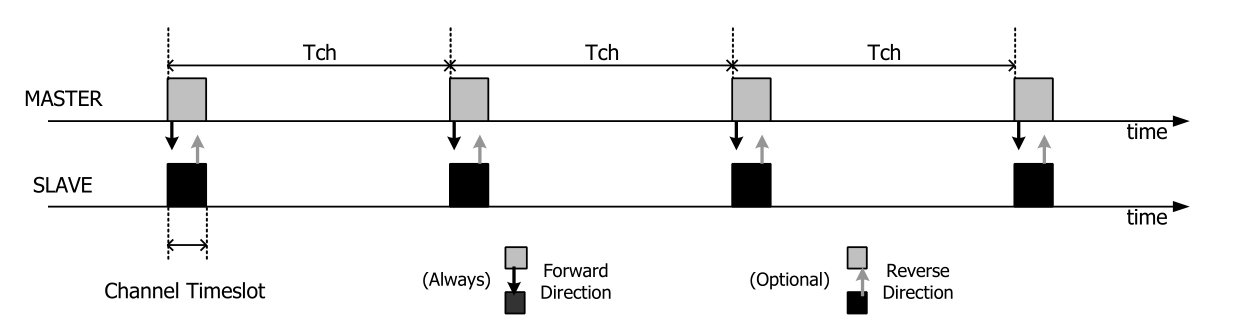
\includegraphics[scale=0.37]{reverse.jpg}
		\caption{Obojsmerná komunikácia po ANT protokole \cite{ANT}.}
		\label{f:reverse_send}
	\end{figure*}


	\begin{figure*}[h]
		\centering
		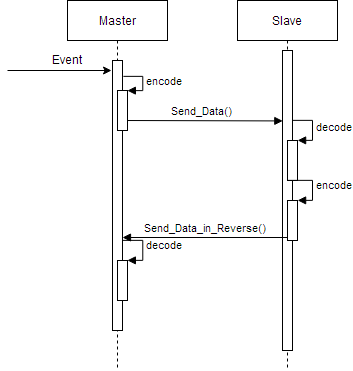
\includegraphics[scale=0.7]{mssequence.png}
		\caption{Komunikácia medzi Master a Slave zariadením.}
		\label{f:mssequence}
	\end{figure*}

\subsection{Master}
	Komunikácia je iniciovaná zariadením, ktoré je nakonfigurované ako Master.
	V periodických časových intervaloch posiela pomocou broadcastov dáta po ANT komunikačnom protokole.
	
	Master je pripojený nRFGo MotherBoard doske a je pripojený k LED diódam a tlačidlám. 
	Pripojenie periférií je nasledovné:
	\begin{itemize}
		\item LED diódy sú pripojené na porte P1,
		\item tlačidlá sú pripojené na porte P2,
		\item ISO7816 signál CLK je pripojený na P0.5,
		\item ISO7816 signál RST je pripojený na P0.4,
		\item ISO7816 signál VCC je pripojený na P0.6,
		\item ISO7816 signál TX je pripojený na P0.3,
		\item ISO7816 signál RX je pripojený na P0.2.
	\end{itemize}

	Master zariadenie umožňuje nakonfigurovať zabezpečenie komunikačného kanála pomocou bootloadera a spustenie automatického testu. 
	Master reaguje na zmenu na tlačidlách a túto zmenu posiela Slave zariadeniu. 
	Dáta prijaté od Slave zariadenie dekóduje a zobrazuje na LED diódach.

\subsection{Slave}
	Slave zariadenie prijíma dáta Master zariadenia. Tieto dáta dekóduje, znovu zakóduje príslušným spôsobom a pošle naspäť Master zariadeniu.
	
	
	Pripojenie periférií je rovnaké ako pri Master zariadení:
	\begin{itemize}
		\item ISO7816 signál CLK je pripojený na P0.5,
		\item ISO7816 signál RST je pripojený na P0.4,
		\item ISO7816 signál VCC je pripojený na P0.6,
		\item ISO7816 signál TX je pripojený na P0.3,
		\item ISO7816 signál RX je pripojený na P0.2.
	\end{itemize}

\section{SW AES}
Za účelom referenčnej softvérovej implementácie AES, bola použitá online dostupná knižnica na GitHube, s názvom Tiny AES128 in C\footnote{\url{https://github.com/kokke/tiny-AES128-C}}. Dĺžka použitého kľúča je 128 bitov. Šifrovanie prebieha v móde CBC.

Kľúč aj inicializačný vektor sú predzdieľané.
Ich hodnoty sú nasledovné:
\begin{itemize}
	\item PSK:    0x2b7e151628aed2a6abf7158809cf4f3c,
	\item vektor: 0xaa55aa55aa55aa55aa55aa55aa55aa55.
\end{itemize}


\section{Bootloader} \label{bootloader}
	Pri podržaní ktorého-koľvek tlačidla ihneď po zapnutí, je možné na Master zariadení, ktorý je osadený na vývojovej doske nRF6310 (nRF Go MotherBoard), nakonfigurovať zabezpečenie bezdrôtového komunikačného kanála. Následne umožňuje zapnutie automatického testu a prejdenie do testovacieho módu na odladenie komunikácie cez štandard ISO7816.
Pre namapovanie týchto funkcií na príslušné tlačidlá viď. \ref{f:o_bootloader}.
	
	Slave zariadenie na sieti sa automaticky prispôsobí nastavenému typu zabezpečenia komunikačného protokolu.
\begin{figure*}[!htb]
	\centering
	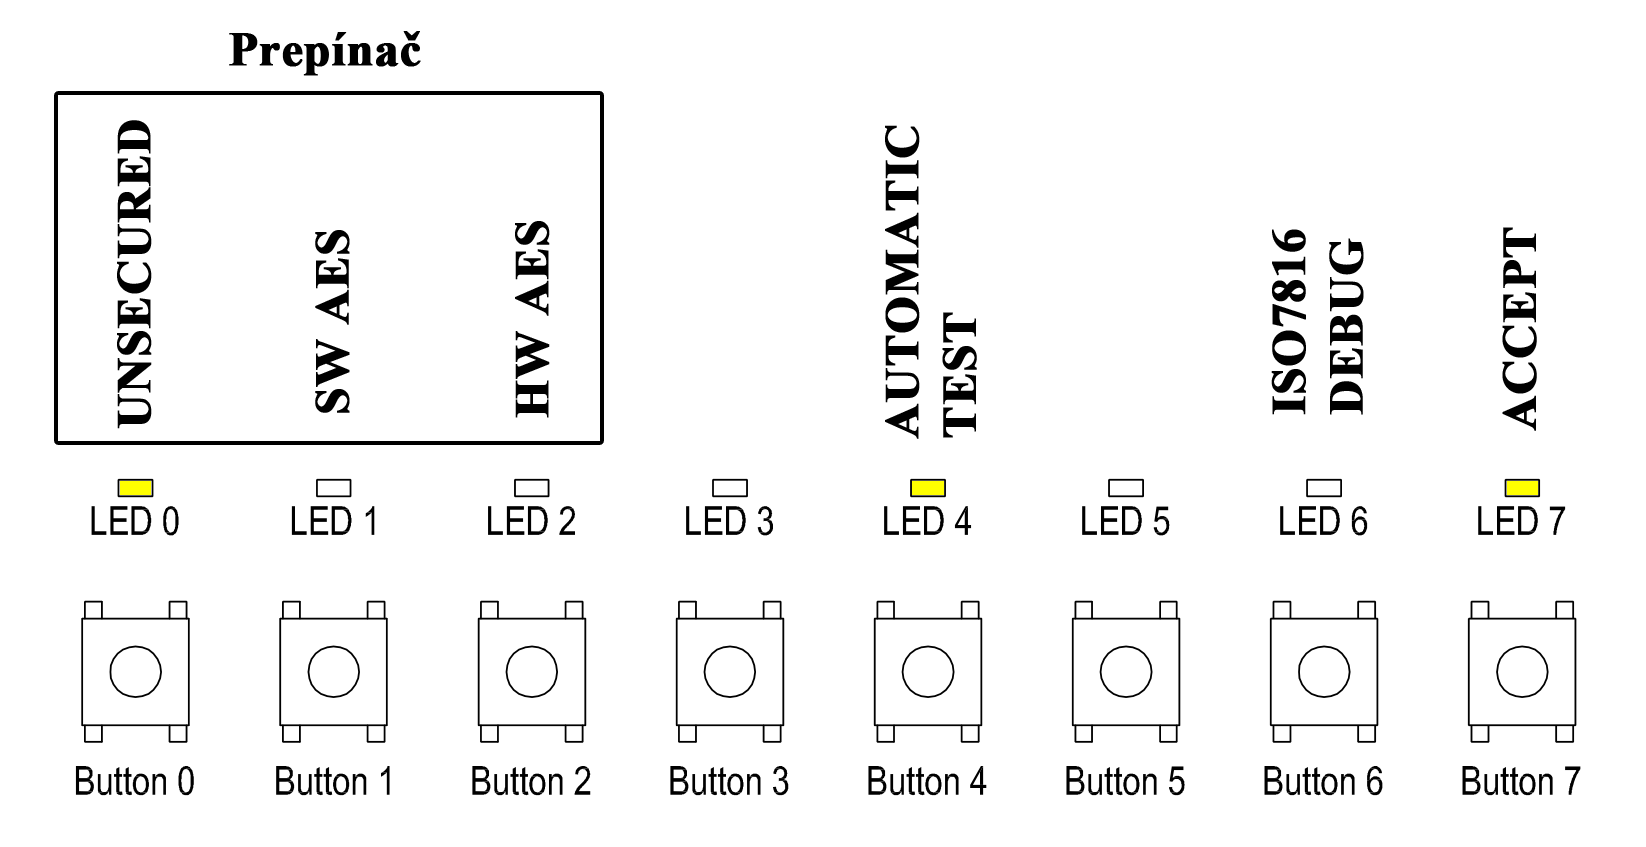
\includegraphics[scale=0.2]{bootloader.png}
	\caption{Konfigurácia nastavení po zapnutí\cite{nrfug}.}
	\label{f:o_bootloader}
\end{figure*}

\section{Štandard ISO7816}

Pre komunikáciu s kryptoelementom bolo nutné naimplementovať rozhranie podľa štandardu ISO7816.

Implementované rozhranie dokáže komunikovať s protokolom, ktorý je kódovaný v priamej konverzií. TS byte Direct conversion ATR 3B
inverse konverzia ATR 3F

Dokáže rozanalyzovať prijímanú ATR správu podľa normy ISO7816 obr. \ref{f:atr}, nie všetky hodnoty sa však používajú.

	\begin{figure*}[h]
		\centering
		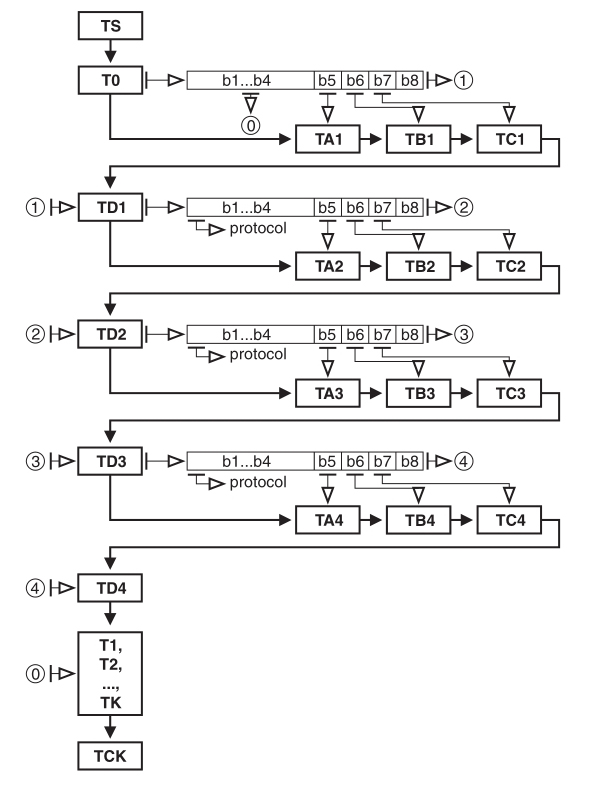
\includegraphics[scale=0.45]{atr_parsing.jpg}
		\caption{Parsovanie ATR (Answer to reset) správy po pripojení smart karty\cite{smartcard}.}
		\label{f:atr}
	\end{figure*}

Program generuje valídne sekvencie studenej aktivácie karty a deaktivácie karty podľa štandadu.

Na generovanie napájania je signál VCC pripojený GPIO pin procesora.
Signál Reset je takisto pripojený na pin procesora.
Generovanie hodinového signálu je realizované procesorom. Generovanie signálu prebieha automatizovane pomocou časovača Timer2 v 8 bitovom režime, udalostí a periférie s názvom PPI (Programmable Peripheral Interface). Pomocou týchto periférií bolo možné vygenerovať pri frekvencií oscilátora 16MHz hodiny s frekvneciou maximálne 4MHz. Výsledný pracovný cyklus hodín je 50\%. Vo výslednej implementácií je frekvencia externého hodinového signálu CLK 2666666.7 Hz.
\ref{f:isouart}

	\begin{figure*}[h]
		\centering
		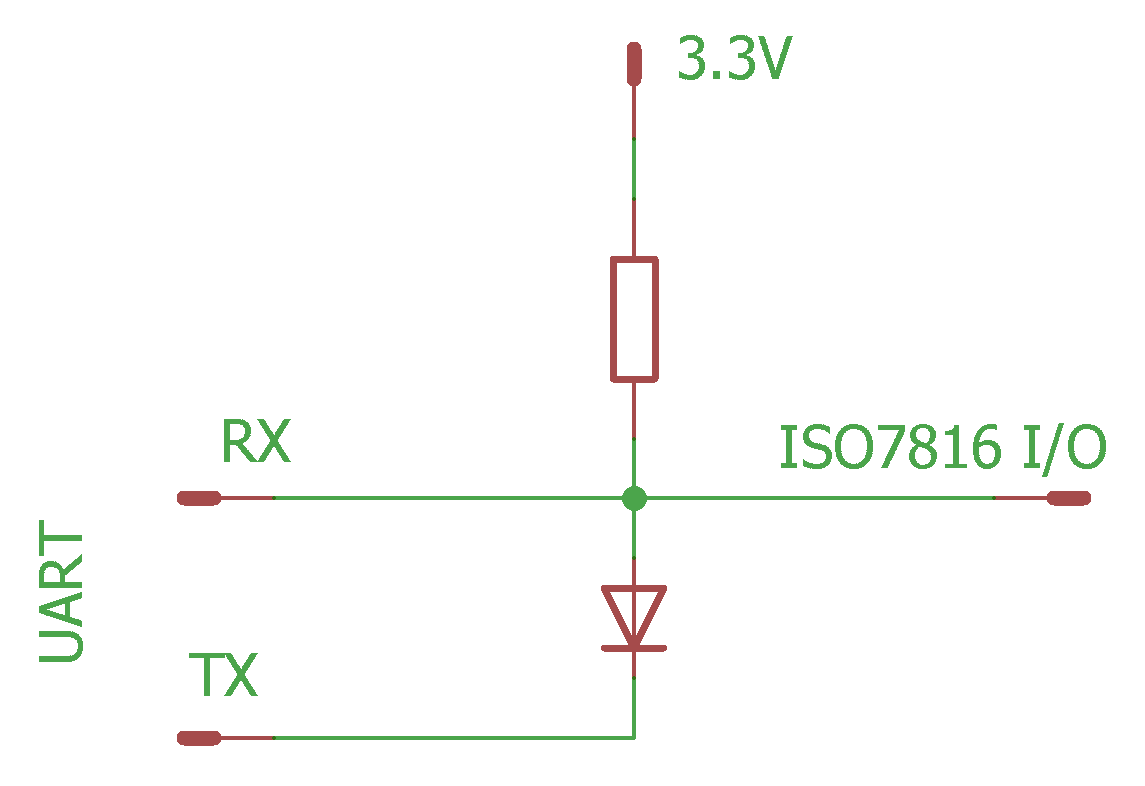
\includegraphics[scale=1.2]{ISOUART.png}
		\caption{Pripojenie pinov RX a TX (UART) k pinu I/O (ISO7816).}
		\label{f:isouart}
	\end{figure*}


pri parametr 372 a 1 je výsledná rýchlosť sériovej linky 7168 bps.

Z analyzovania správy. Program umožnuje aj vyjednávanie zmeny protokolu, vo výsledku sa ale nepoužíva a komunikuje sa protokolom, ktorý preferuje daný kryptoelement alebo smart karta.

Z ATR správy okrem iných vecí, sa dá identifikovať preferovaný spôsob a parametre komunikácie. Boli implementované dve najpoužívanejšie formy komunikácie štandardu ISO7816-3:
	\begin{itemize}
		\item Bajtovo orientovaný prenos dát T=0: forma a štruktúra posielaných dát vo forme APDU je na obr.  \ref{f:apdu},
		\item blokovo orientovaný prenos dát T=1: forma a štruktúra posielaných dát vo forme bloku je na obr. \ref{f:tpdu}. Štandardne sa do bloku zabaľujú dáta vo forme APDU správy \ref{f:apdu}. Štandardne je v blokovej komunikácií použitý spôsob kontrolnej sumy vo forme LRC (longitudinal redundancy check), ktorý vyžaduje jeden bajt. Dvoj-bajtové CRC so špecifickým polynómom nebolo nutné implementovať. Následne je implementované sekvenčné číslo pri komunikácií podľa protokol T=1.
	\end{itemize}


	\begin{figure*}[h]
		\centering
		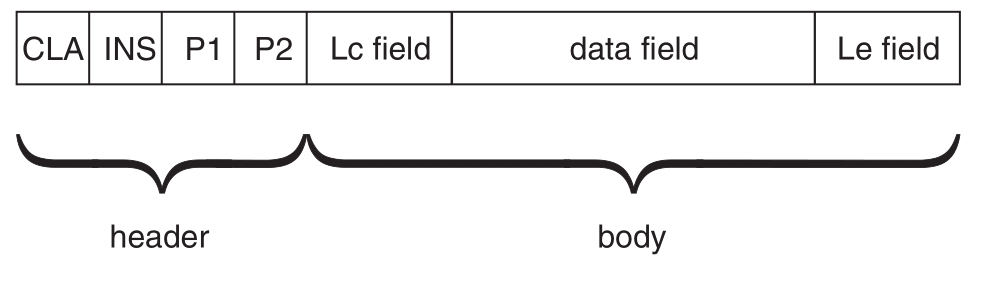
\includegraphics[scale=0.2]{apdu.jpg}
		\caption{Štandardný format APDU správy podľa štandardu ISO7816\cite{smartcard}.}
		\label{f:apdu}
	\end{figure*}
	
	\begin{figure*}[h]
		\centering
		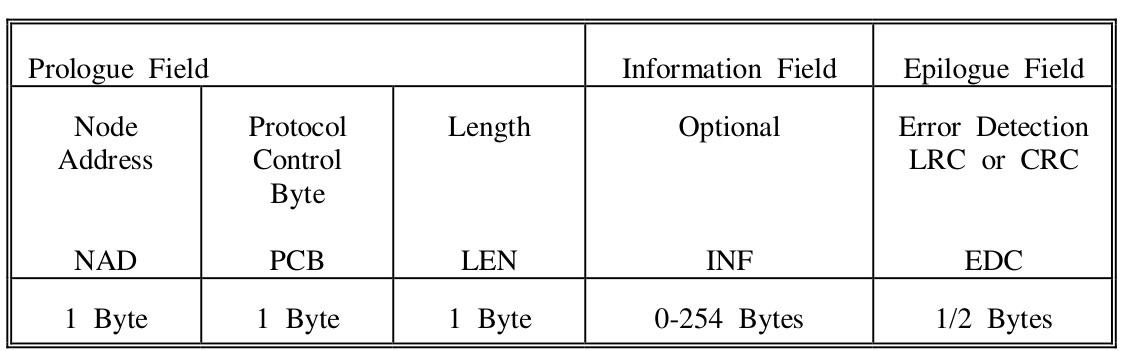
\includegraphics[scale=0.2]{block.jpg}
		\caption{\cite{SmartCardTutorial}.}
		\label{f:tpdu}
	\end{figure*}


Z viacerých zdrojov na internete boli pozbierané štandardné odpovede protokolu spolu s ľudsky čitateľnou správou, čo reprezentujú. Tieto odpovede majú veľký význam pri odlaďovaní komunikácie. Odpovede spolu s príslušnými hláškami sú zozbierané v súbore /Keil/ISO7816\_errors.h.h


\section{ISO7816 debugger}
pripojenie
cez jlink rtt viever
	CLK
	Reset
nastavnie baudrate
aktivacia deaktivacia, restovanie,
nastavenie parity
T=0 T=1
obrazok
posielanie sprav zadanych cez segger konzolu

vyhladavanie card manazera  a prehladavanie instruckcii
\ref{f:i_iso_dekoder}

\section{Applet}

PSK
vector

AES
toto áno
toto nie
krpytoelementy ake typy a oznacenie

Boli vyskusane rozne verzie Eclipse, JRE, JCKITu, a rozne typy konvertorov na vysledny cap súbor.  Specificky kompilator a nastavenie. Výsledný funkčný postup je opísaný v kapitole \ref{s_applet_compile}.

odpoveda na nasledujuce apdu spravy v datovej cast. Na parametroch apdu spravy ako Instrukcia, parametre P1 a P2 nezalezi, neberu sa do uvahy.
\begin{itemize}
	\item FF odpovie aa test odpovede appletu a kryptoelementu
	\item 03 16 bajtov zakoduje 
	\item 04 16 bajtov
	\item ak prijme cokolvek ine, posle v odpovedi rovnake data ako prijal v apdu sprave.
\end{itemize}


\section{Automatizovaný test}
Princíp automatického testu, spočíva v tom, aby boli zabezpečené konzistentné podmienky počas meraní, pri rôznych typoch zabezpečenia komunikačného kanála.

Počas automatického testovania, Master zariadenie neprijíma udalosti z tlačidiel, ale dáta ktoré sa posielajú po komunikačnom protokole sú generované programovo. Master odošle zakódovanú hodnotu, začínajúcu na nule, Slave zariadeniu. Ten by ju mal poslať naspäť. Pokiaľ však Master nepríjme dáta do istého časového okamžiku, alebo príjme iné dáta ako poslal pri poslednom odoslaní, pokúsi sa správu poslať znovu. Pokiaľ bola naspäť prijatá správa s rovnakým obsahom, ako bola poslaná, inkrementuje sa posielaná hodnota, ktorá sa znova odošle.

Test sa ukončí po úspešnom vykonaní určitého počtu cyklov odoslaní a prijatí, ktorý sa nastavuje parametrom TEST\_MAX\_VALUE počas kompilácie.

Každá prijatá hodnota sa súčasne vykreslí na LED diódy.

\section{Dosky plošných spojov}
Počas vypracovania záverečnej práce boli navrhnuté, vyrobené a osadené dve dosky plošných spojov. Ich zapojenie a funkcie sú opísané v nasledujúcich kapitolách.

	\subsection{Testovacia doska pre štandard ISO7816}
	
	Prvá navrhnutá a realizovaná doska, slúži v prvom rade na odladenie komunikácie prostredníctvom UART sériovej linky so štandardom ISO7816 a na pozorovanie správania sa komunikácie s rôznym spôsobom pripojenia sériovej linky ku kryptoelementu.
	
	Konektor vľavo (obr. \ref{f:board_ISO_schematic}) slúži na pripojenie pinov procesora. Na konektor vpravo sa pripojuje kryptoelement alebo smart karta štandardom ISO7816.
	
	Prvý jumper vľavo (\ref{f:board_ISO_schematic})  umožnuje odpojiť a pripojiť signál TX, na signál RX sériovej linky. A to buď cez rezistor alebo diódu.
	Pomocou druhého jumpra je možné odpojiť alebo pripojiť dva typy pull-up rezistorov na I/O linku. Hodnoty osadených rezistorov sú 10k a 3k3. 
	Väčšina literatúry, týkajúca sa zapojenia a komunikácie so smart kartami, odporúča mať pripojený  pull-up odpor na komunikačnú linku. Hodnota napájania na pull-up odporoch, by mala odpovedať maximálnemu dovolenému napätiu, ktoré smart karta podporuje: 1.8V, 3.3V alebo 5V.
	
	Pomocou týchto jumprov je možné testovať rôzne kombinácie zapojení. Vo výslednom zapojení, aj na druhej doske bolo použité zapojenie zobrazené na obr. \ref{f:isouart}.
	
	 V rozložení súčiastok na doske, obr. \ref{f:board_ISO_layout}, boli pridané testovaci body, napr. pre pripojenie multimetrov a osciloskopu.
	
	Výsledná doska je zobrazená na obr.  \ref{f:i_board_iso}.
	
	\begin{figure*}[h]
		\centering
		\includegraphics[scale=0.7]{Schematics.png}
		\caption{Testovacia doska pre konverziu UART na štandard ISO7816.}
		\label{f:board_ISO_schematic}
	\end{figure*}
	
	\begin{figure*}[h]
		\centering
		\includegraphics[scale=1]{Board.png}
		\caption{Rozloženie súčiastok na doske plošných spojov.}
		\label{f:board_ISO_layout}
	\end{figure*}
	
	\subsection{Doska pre Slave zariadenie}

	Hlavný prínos dosky pre Slave zariadenie je v tom, že poskytuje napájanie pre vývojový kit od spoločnosti Nordic. Doska má osadený aj vyhladzovací kondenzátor.
	Doska je napájaná napätím 3.3V.
	
	Druhá funckionalita, ktorú doska poskytuje je pripojenie UART sériovej linky k štandardu ISO7816, podľa schémy zapojenia, ako je na obr. \ref{f:isouart}. Všetky signály potrebné pre komunikáciu podľa štandardu ISO7816, ktoré procesor generuje, sú pripojené k portu P0 a vyvedené k príslušnému konektoru.
	Schéma zapojenia dosky pre Slave zariadenie je na obr. \ref{f:board_slave_schematic}. 
	
	Vývojový kit Nordic, má použité menej tradičné konektory, na pripojenie sa k rozširujúcej doske nRF Go Motherboard. To zťažilo pripojenie kryptoelementu k vývojovému kitu. Protichodný konektor nebol dostupný v bežných predajniach a vyskytoval sa iba v prevedeniach SMD. 
	Rozteč medzi jednotlivými pinmi konektoru je dosť malá (1.27mm), aby sa s nimi dalo efektívne pracovať v domácich podmienkach. Pri výrobe totiž nemusí prísť k dokonalému preneseniu stôp z prenového média (papier), na dosku plošných spojov. V domácich podmienkach takisto veľmi ľahko môže prísť k podleptaniu a súčasne aj k nedostatočnému odleptaniu medenej vrstvy. Bolo teda nutné vymyslieť vlastný konektor.	
	
	Vo vývojovom nástroji Eagle, bola vytvorená vlastná knižnica, pre daný konektor (2x20 pinov), ktorá slúži hlavne ako vodítko, v akých vzdialenostiach sa majú konektory nachádzať a ďalej vyznačuje miesta, kde majú byť odvŕtané diery a pripojené vodiče.
	
	Vodiče sú v konektore uložené voľne. Vodiče sú následne v dostatočnej vzdialenosti pripájkované k správnym cestám. Najideálnejšie pasovali do protichodného konektora na Nordic doske, jednožilové medené vodiče z eternetového kábla.
	
	Tímto štýlom je privedené napájanie a zem k doske, spolu so signálmi pre štandard ISO7816. 
	
	Výsledné cesty spolu s osadením súčiastok sú na obr. \ref{f:board_slave_layout}.
	
	Detail zapojenia a pripojenia konektora je zobrazený na obr. \ref{f:i_board2}.
	Výsledná osadená doska spolu s pripojeným vývojový kitom je zobrazená na obr. \ref{f:i_board_nrf}.
	
	\begin{figure*}[h]
		\centering
		\includegraphics[scale=0.7]{test2.png}
		\caption{Schéma zapojenia a pripojenia slave zariadenia s kryptoelementom.}
		\label{f:board_slave_schematic}
	\end{figure*}
	
	\begin{figure*}[h]
		\centering
		\includegraphics[scale=1]{test.png}
		\caption{Rozloženie súčiastok na doske plošných spojov pre slave.}
		\label{f:board_slave_layout}
	\end{figure*}

\section{Projekt}
	Include obsahuje vsetky hlavickove subory a subory s externym kodom, ktore su potrebne pre dany projekt.
	
	Projekt ma v sebe nakonfiguronve , paramtre kompilovanie, pouzity SoftDevice program a data.
	Nastavenia pre nahratie a odladenie programu s pouzitim Segger programatora. Rozsahy pamati pre 
	
	Projekt vo vyvojovom prostredi ma predkonfigurovane rozne ciele. Tzn. ze z jedneho projektu je mozne skopilovat rozne a odladovat iba jedntlive izolovane funckionality. Subory, ktore spolu logicky suvisia su spolu zadefinovane  v skupinach.
	
	Kazdy target moze mat nastavene rozne parametre kompilovania, subory, ktore sa maju skopilova a aj rozdielne typy includov.
	
	\ref{f:keil_project}
	
	Opis typov cieľových zariadení pri kompilácií:
	\begin{itemize}
		\item Master
		\item Slave
		\item Converter
		\item Converter
	\end{itemize}
	
	Opis najdoležitejších súborov v projekte:
	\begin{itemize}
		\item a
	\end{itemize}

	\begin{figure*}[h]
		\centering
		\includegraphics[scale=0.35]{i_projekt1.jpg}
		\caption{Nahratie appletu na kryptoelement.}
		\label{f:keil_project}
	\end{figure*}

%TODO
%Popisuje vybrané dôležité časti kódu.
%Štruktúra Certifikátu
%Použité referenčné softvérové implementácie RSA a AES v jazyku C.

\chapter{Testovanie} \label{s_testing}
Kapitola testovania sa zaoberá návrhom vhodných testov, vybraním vhodných parametrov, ukazovateľov a samotnou realizáciou testov. Následne sa zaoberá porovnaním a vyhodnotením získaných dát.
Pri navrhovaní testov boli uvažované viaceré metriky: rýchlosť kryptovania a dekryptovania, prúdová spotreba zariadenia a výdrž zariadenia napájeného batériou. Doba odozvy, dáta prenesené navyše po sieti, nároky na prenosové komunikačné pásmo, odozvu a oneskorenie zariadenia od prijatia požiadavky až po jej vykonanie a spracovanie, zabezpečenie kvality služieb, pamäťové nároky na rôzne typy pamäti ako ROM, RAM.
Veľkosti pamäťových nárokov sa zisťujú priamo z výstupu kompilátora. Nároky na sieť sú vypočítané z veľkosti dát a štruktúr, ktoré sú potrebné pri naviazaní a zabezpečení spojenia medzi uzlami.
Prúdová spotreba je meraná externým DMU s rozumnou precíznosťou a kalibráciou.
Čas vykonávania programu je meraný externe, počítadlom impulzov alebo frekvencie a následne porovnaním s dĺžkou vykonávania programu získanou priamo z meraného obvodu, z príslušného časovača alebo hodín reálneho času napr. cez rozhranie UART alebo RTT.

%\section{}
Realizovanie testov prebieha v troch hlavných fázach, ktoré sú medzi sebou porovnané:
\begin{itemize}
	\item bez zabezpečenia: dáta sú po sieti prenášané bez akéhokoľvek zabezpečenia, autentifikácie zariadení a podobne,
	\item so softvérovým zabezpečením: kryptografické algoritmy sú realizované referenčnými implementáciami pre jazyk C,
	\item s hardvérovým zabezpečením: kryptografické algoritmy sú realizované špecializovaným dedikovaným externým zariadením.
\end{itemize}
\onehalfspacing

Testovanie zabezpečenia prebieha pomocou troch rôznych spôsobov kryptovania:
\begin{itemize}
	\item čistá symetrická kryptografia: zabezpečuje dôvernosť a integritu ale nie autentifikáciu,
	\item čistá asymetrická kryptografia: realizovaná napr. pomocou RSA alebo eliptických kriviek, ktorá už dokáže zabezpečiť aj autentifikáciu zariadení,
	\item kombinácia asymetrickej a symetrickej kryptografie: asymetrická kryptografia sa použije na výmenu symetrického kľúča, ktorý sa pravidelne mení a môže byť generovaný a distribuovaný rovnaký pre skupinu logicky súvisiacich zariadení.
\end{itemize}
\onehalfspacing


Aby sa zabezpečila relevantnosť výsledkov, je vykonaných niekoľko opakovaných meraní, ktoré sú následne spriemerované a sprevádzané s výpočtom smerodajnej odchýlky.

Porovnanie medzi hardvérovými a softvérovými implementáciami bude prebiehať nad rovnakým objemom a obsahom dát. Mení sa iba spôsob implementácie zabezpečenia siete.

Výsledky meraní sú zapísané do tabuľky \ref{t:t_testovanie} a následne vyhodnotené.

%\begin{adjustbox}{angle=90}

	\begin{table}[h]
		\centering
		\caption{Tabuľka pre zápis výsledkov z testovania.}
		\label{t:t_testovanie}
		\Rotatebox{90}{
			\begin{tabular}{|c|l|l|l|l|l|l|}
				\hline
				\multirow{2}{*}{Implementácia} & \multicolumn{1}{c|}{\multirow{2}{*}{Typ zabezpečenia}} & \multicolumn{5}{c|}{Metriky} \\ \cline{3-7} 
				& \multicolumn{1}{c|}{} & \multicolumn{1}{p{3.1cm}|}{Pamäť programu {[}B{]}} & \multicolumn{1}{p{1cm}|}{RAM {[}B{]}} & \multicolumn{1}{p{3.3cm}|}{Prúdová spotreba {[}mA{]}} & \multicolumn{1}{p{1cm}|}{Čas {[}ms{]}} & \multicolumn{1}{p{3.5cm}|}{Network overhead {[}B{]}} \\ \hline
				& Žiadne zabezpečenie &  &  &  &  &  \\ \hline
				\multirow{3}{*}{SW} & AES 128 &  &  &  &  &  \\ \cline{2-2}
				& RSA/ECC &  &  &  &  &  \\ \cline{2-2}
				& RSA/ECC + AES &  &  &  &  &  \\ \hline
				\multirow{3}{*}{HW} & AES 128 &  &  &  &  &  \\ \cline{2-2}
				& RSA/ECC &  &  &  &  &  \\ \cline{2-2}
				& RSA/ECC + AES &  &  &  &  &  \\ \hline
			\end{tabular}
		}
	\end{table}
%\end{adjustbox}
\chapter{Zhodnotenie} \label{s_conclusion}
%\section{Záver}
%Zanalyzovali sme kryptograficke algoritmy, protokoly, dostupne bezne technologuie.
%Napln prace v dalsom semestri bude spocivat v doplneni a uprave uz vytvorených kapitôl. Budeme sa viac venovať samotnému podrobnejsiuemu navrh, kde sa budeme snazit zabezpecit siet a uzly pre tpymi utokov.

Zhodnotenie sa venuje vyhodnoteniu jednotlivých fáz vypracovania záverečného projektu. Uvádzajú sa vzniknuté problémy počas jednotlivých fáz vypracovania, stručné zhodnotenie, čo sa podarilo, nepodarilo a aké sú možnosti a priestory na vylepšenia.

\section{Zhodnotenie prvej fázy vypracovania projektu}
V prvej časti vypracovania záverečného projektu sme sa zamerali na čo najširšie zanalyzovanie a oboznámenie sa s komplexnou problematikou spojenou s bezpečnosťou. Študovali sme motiváciu, rozmýšlanie rôznych typov útočníkov, analyzovali sme ich metódy a nástroje. Zaoberali sme sa taxonómiou realizovania aktívnych útokov na rôzne typy systémov, nielen bezdrôtové komunikačné siete. Následne oblasťami ako informačná bezpečnosť, aktuálnym trendom hardvérového zabezpečenia v rôznych oblastiach a riešeniami od dodávateľov ako Microchip\footnote{\url{http://www.microchip.com/design-centers/internet-of-things}} alebo Atmel\footnote{\url{http://blog.atmel.com/2015/11/09/develop-secure-iot-apps-with-the-atmel-certified-id-platform/}} pre oblasti ako IoT. Zamerali sme sa aj na aktuálne vyvíjané technológie, bezpečnostými slabinami systémov, získavaním root oprávnení rôznych zariadení, kryptografickými algoritmami, dostupnými bezdrôtovými komunikačnými protokolmi a používanými zariadeniami v inteligentných domácnostiach.

%Bola analyzovana do istej miery bezpocnost spojena s bezdorovymi komunikacnymi sietami

Snažili sme sa získať predstavu, ako by mal celý systém fungovať a aké sú predpoklady od jednotlivých zúčastnených strán, aby sme navrhli a aplikovali správne resp. vhodné protiopatrenia.
Spravili sme si celkový široký pohľad na problematiku a navrhované riešenie na rôznych úrovniach abstrakcie, od fyzickej vrstvy navrhovaného systému, ich fungovanie, vzájomné poprepájanie, limitácie, až po aplikačné vrstvy ako je ochrana aktív a informácií. Pozerali sme sa na systém, ako realizátor projektu, ktorého zaujíma cena, čas potrebný na nasadenie produktu, znovupoužiteľnosť komponentov, jednoduchá rozšíriteľnosť siete a služieb v sieti, až po bežného koncového spotrebiteľa, ktorý má isté predpoklady o fungovaní systému a bude náš systém používať. Pri koncovom používateľovi treba myslieť na použiteľnosť systému, funkčnosť, výslednú celkovú bezpečnosť, používateľský zážitok, jednoduchosť použitia, možnosť konfigurácie, manažovania, pridávanie a odoberanie zariadení.

Následne boli analyzované najpoužívanejšie dostupné kryptrografické algoritmy.
Analyzované boli dostupné a používané bezdrôtové komunikačné protokoly.
Pozreli sme sa na dostupné produkty z oblasti domácej automatizácie a ich zabezpečenie.

Zamerali sme sa aj na problematiku návrhu bezpečných vnorených aplikácií v podobe appletov pre platformu Java Card Open Platform.

Bola vykonaná hĺbková analýza širokej problematiky spojenej s návrhom a bezpečnosťou inteligentných domácností.
Bol zadefinovaný pojem inteligentná domácnosť, jeho hlavné prvky a aké prináša výhody.

Vykonali sme blokový návrh fungovania, architektúry a topológie navrhovanej inteligentnej domácnosti a zadefinovali sme použité uzly v sieti. Zadefinovaným prvkom siete sme pridelili základné funkcionality. Spravili sme si predstavu, ako bude navrhovaný systém fungovať ako celok, identifikovali sme proti komu stojíme a akým spôsobom sa snažíme zabezpečiť bezpečnostné parametre siete.

Zostáva sa zamyslieť nad cenou a dopadmi zabezpečenia detekcie alebo prevencie proti fyzickým útokom, napr. pri komunikácií riadiaceho mikropočítača so secure elementov, zaliatím zariadenia do epoxidu, realizovaním zariadenia ako SiP (systém v púzdre), alebo pomocou iných metód požívaných vo vojenských aplikáciach. Pri návrhu bezpečnostných systémov netreba zabúdať ani na písanie bezpečného softvéru odolného proti aktívnym fyzickým útokom a softvéru so zvýšeným zabezpečením proti poruchám.

V nasledujúcej etape dopracujeme vybrané časti analýzy, porovnáme analyzované protokoly v tabuľke, dopracujeme návrh a začneme sa venovať implementácií a návrhu testov.

%\cite{networksecurity}.
\section{Zhodnotenie druhej fázy vypracovania projektu}
V druhej časti vypracovania diplomového projektu sme upravili a prerobili niektoré časti vybraných kapitol. Do istej miery bol upravený návrh. Boli dopracované kapitoly týkajúce sa kryptografie, bezdrôtovými komunikačnými protokolmi, implementácie a kapitola týkajúca sa testovaním a vyhodnotením nameraných výsledkov. Navrhli sme spôsob realizovania testovania a overenie riešenia.

Oboznámili sme sa do istej miery s hardvérom a jeho architektúrou. Začali sme s implementáciou od spojazdnenia programátora a vývojových prostredí, cez zabezpečenie odľadovania programu, jednoduchého rozblikania lediek, načítania vstupov z tlačidiel až po štúdium aplikačných rozhraní pre prácu s protokolovým zásobníkom na komunikáciu po bezdrôtovom komunikačnom kanále.

Predpokladaný plán práce a rozloženie úloh v ďalšom semestri je v prílohe v tabuľke \ref{t:plan_prace}.


\section{Zhodnotenie tretej fázy vypracovania projektu}
nepodarilo sa mi nasjt a spojazdnit sw knizcniu pre vypocet. Hladal som specificku, taku, ktora bude jednoducha v zmysle pouzivania statickym poli a nie dynamickej alokacie pocas behu programu, 


Vzhladom na to, ze implementacia a odladenie komunikacie podla standardu ISO7816 trvala dlhsie ako som predpokladal, a neskor sa vyskytli este problemy so specifickou kompilaciu a vyzadovala specificke nastavenia systyemu, aby kryptoelemeny prilaj pri Load instruckii skompilovany applet, 

Porovnaj to s hw implementaciou

zavisi od ryclhosti seriovej linky

Doimplementovat 
Vyskusat rozne rychlost
Externe generovanie CLK signal 3.5 5 10 MHz v zavilsto od fyzickych limitov niektorcychsmart kareit

\section{Zhodnotenie}
Podarilo sa uspense doimplementovat obosmernu komuniaciu pomocou ANT protokolu, naimplelemtntovať a oddebugovat komunikaciu podla standardu ISO7816, naimplementovat a nahrat applet na kryptoelemnt, obashujuci Java VM A vyuzit kryptograficke funkcie tohto appletu na zakodovnaie dát.
Naimplementovat posielanie sprav cez vaic casovych okien ANT komunikacneho protokolu. Takisto boli navrhnute a vyrobene 2 dosky polosnych spojov pre pripojenei kryptoelementu a nordic vyvojového kitu.

Spociatku som bol skepticky, nakoniec aj pri horšich vysledok, tato komunikacia je standardizovana, pravidelene revidovana, umoznuje v podstate cokolvek co si zmyslyte. Vypocty PKI, ECC, nasobenie velkych cisiel, kryptograficku podporu, externu pamat, koprocesor, viac appletov na danej smart karte, parametrizaciu, bezpecne ukladanie, pristup k dodatocnym rozhraniam ako napr NFC, si myslim, ze v specifickych pripadoch prenositelenost na ostatne zariadenie, ktore dany standard pouzivaju.

Secure messaging medzi zariadenim a smart kartou

Vyhodnotenie vysledkov

%\section{Zhodnotenie poslednej fázy vypracovania}
%Co sa podarilo,
%Co sa nepodarilo
%Napady na vylepsenia
%V com mozu pokracovat dalej

\clearpage
\phantomsection
\addcontentsline{toc}{chapter}{Použitá literatúra}
%\printbibliography
\bibliography{literatura}
\bibliographystyle{siam} %plain siam

%\newpage
%\mbox{}

\newpage
\thispagestyle{empty}
\vspace*{10cm}
\hspace*{5cm}
\textbf{\LARGE{PRÍLOHY}}

\addappheadtotoc
\def\appendixname{}
\appendix

\newpage
\pagenumbering{bychapter}

\chapter{Plán práce v DPIII}
\begin{table}[h]
	\centering
	\caption{Plán práce v DPIII}
	\label{t:plan_prace}
	\noindent\begin{tabular}{|c|c|c|l|}
		\hline
		\multicolumn{1}{|c|}{} & \multicolumn{1}{c|}{Začiatok} & \multicolumn{1}{c|}{Koniec} & {Plánovaná náplň práce} \\ \hline
		\multirow{2}{*}{Február} & 13.2. & 19.2. & \multirow{3}{*}{\parbox{10cm}{SW implementácie kryptografických metód}} \\
		& 20.2. & 26.2. &  \\ \cline{1-3}
		\multirow{4}{*}{Marec} & 27.2. & 5.3. &  \\ \cline{4-4} 
		& 6.3. & 12.3. & \multirow{3}{*}{\parbox{10cm}{Implementácia appletov pre komunikáciu s kryptoelementom}} \\
		& 13.3. & 19.3. &  \\
		& 20.3. & 26.3. &  \\ \hline
		\multirow{5}{*}{Apríl} & 27.3. & 2.4. & \multirow{3}{*}{\parbox{10cm}{Použitie HW  kryptoelementov na bezdrôtovú komunikáciu}} \\
		& 3.4. & 9.4. &  \\
		& 10.4. & 16.4. &  \\ \cline{4-4} 
		& 17.4. & 23.4. & \multirow{4}{*}{\parbox{10cm}{Testovanie, porovnanie výsledkov, finalizácia dokumentu, vyhodnotenie}} \\
		& 24.4. & 30.4. &  \\ \cline{1-3}
		\multirow{2}{*}{Máj} & 1.5. & 7.5. &  \\
		& 8.5. & 11.5. &  \\ \hline
	\end{tabular}
\end{table}

%\newpage
%\pagenumbering{bychapter}
%\chapter{Technická dokumentácia a používateľská príručka}
%\subsection

\newpage
\pagenumbering{bychapter}
\chapter{Obsah priloženého média}
Priložené elektronické médium má nasledovný obsah a štruktúru:
%\begin{verbatim}
%\end{verbatim}

\begin{tikzpicture}[dirtree, scale=0.5]
	\node {\textbf{root}} 
	child { node {\textbf{Anotácia}}
			child { node {AnotaciaSJ.pdf} }
			child { node {AnotaciaEN.pdf} }
	}
	child { node {\textbf{Titulná strana}}
		child { node {titulna\_strana.pdf} }
	}
	child { node {\textbf{Dokumentácia}}
		child { node {\textbf{Obrázky}} }
		child { node {Dokument.pdf} }
		child { node {Dokument.tex} }
		child { node {Literatura.bib} }
	}
	child { node {\textbf{Applet}}
		child { node {\textbf{Applet}}
			child { node {\textbf{src}}
					child { node {\textbf{test}} 
							child { node {Test.java}}
					}
    		}
    	}
		child { node {\textbf{GPShell}} }
		child { node {\textbf{Install}} 
					child { node {test.cap} }
					child { node {applet\_install.txt} }
					child { node {applet\_try.txt} }
					child { node {applet\_delete.txt} }
			}
		child { node {\textbf{JDCE}} }
		child { node {\textbf{JDCK222}} }
		child { node {\textbf{JDK160}} }
	}
	child { node {\textbf{DPS dosky}}
		child { node {\textbf{Knižnica}}
			child { node {sfc-120-t2-l-d.lbr} }		
		}
		child { node {dp.sch} }
		child { node {dp.brd} }
		child { node {dpMaster.sch} }
		child { node {dpMaster.brd} }
	}	
	child { node {\textbf{Referenčné softvérové implementácie}}
			child { node {tiny-AES128-C-master.zip} }
	};
\end{tikzpicture}

\begin{tikzpicture}[dirtree, scale=0.5]
	\node {\phantom{    }} 
	child { node {\textbf{Keil}}
		child { node {\textbf{Include}} }
		child { node {Universal.h}}
		child { node {ISO7816.h}}
		child { node {ISO7816\_errors.h}}
		child { node {EncryptionType.h}}
		child { node {PSK.h}}
		child { node {ANT\_SD.c}}
		child { node {Automated\_Test.c}}
		child { node {Bootloader.c}}
		child { node {CLK\_Gen.c}}
		child { node {CLK\_Gen\_functions.c}}
		child { node {EncodeDecode.c}}
		child { node {GlobalInit\_functions.c}}
		child { node {Globals.c}}
		child { node {GPIO\_functions.c}}
		child { node {ISO7816\_activation\_sequences.c}}
		child { node {ISO7816\_APDU\_tests.c}}
		child { node {ISO7816\_Applet\_Communication.c}}
		child { node {ISO7816\_Applet\_functions.c}}
		child { node {ISO7816\_ATR\_functions.c}}
		child { node {ISO7816\_error\_functions.c}}
		child { node {iso7816\_functions.c}}
		child { node {ISO7816\_init.c}}
		child { node {ISO7816\_Message\_Checks.c}}
		child { node {ISO7816\_Messages\_functions.c}}
		child { node {ISO7816\_Misc\_functions.c}}
		child { node {ISO7816\_Segger\_UART\_7816\_converter.c}}
		child { node {ISO7816\_send\_recieve.c}}
		child { node {ISO7816\_timing\_calc\_functions.c}}
		child { node {ISO7816\_uart\_iso\_converter\_Standalone.c}}
		child { node {main.c}}
		child { node {Master.c}}
		child { node {Misc\_functions.c}}
		child { node {Pin\_RST.c}}
		child { node {Pin\_VCC.c}}
		child { node {Segger\_functions.c}}
		child { node {Segmenter.c}}
		child { node {Slave.c}}
		child { node {UART\_functions.c}}
		child { node {UART\_test.c}}
		child { node {JLinkSettings.ini}}
		child { node {ant\_temp.sct}}
		child { node {ant\_temp.uvopt}}
		child { node {ant\_temp.uvproj}}
	};
\end{tikzpicture}

%child { node {uSD projekt} }

%\end{otherlanguage*}

%tencnicka dokumentacia navom, komipilacia rozbehanie
\chapter{Technická dokumentácia} \label{s_manual}
 
	\section{Nahratie programu na vývojovú dosku Nordic} \label{s_nrf_program}
 \begin{enumerate}
 	\item Nainštalujte vývojové prostredie Keil v edícií MDK-Lite (Microcontroller Development Kit), ideálne verziu 521a\footnote{\url{http://www2.keil.com/mdk5/}},
 	\item nainštalujte nRF51\_SDK verziu 10.0.0, pre Keil nRF5x\_MDK\_8\_2\_0\_Keil4.msi\footnote{\url{https://developer.nordicsemi.com/nRF5_SDK/nRF51_SDK_v10.x.x/}},
 	\item otvorte Keil IDE, doinštalujte a aktualizujte balíčky, ktoré by ste chceli používať (Nordic dosky, ARM kompilátor),
 	\item otvorte projekt nachádzajúci sa na priloženom médiu v priečinku /Keil/,
 	\item vyberte cieľové zariadenie, pre ktoré chcete skompilovať kód,  \ref{f:i_keil_flash} krok 1,
 	\item kliknite na prekompilovať všetko,  \ref{f:i_keil_flash} krok 2,
 	\item pripojte programátor Segger J-Link k nRF doske,
 	\item pripojte nápajanie k doske,
 	\item nahrajte skompilovaný program na dosku, kliknutím na Load \ref{f:i_keil_flash} krok 3.
 \end{enumerate}
 
 \begin{figure*}[!htb]
 	\centering
 	\includegraphics[scale=0.3]{keil_flash.jpg}
 	\caption{Nahratie programu na vývojovú dosku.}
 	\label{f:i_keil_flash}
 \end{figure*}
 
 \newpage
 
\section{Skompilovanie appletu} \label{s_applet_compile}
	\begin{enumerate}
		\item Rozbaľte JCDK 2.2.2 development kit\footnote{\url{http://www.oracle.com/technetwork/java/embedded/javacard/downloads/javacard-sdk-2043229.html}},
		\item nainštalujte Eclipse 3.5 (Galileo)\footnote{\url{http://archive.eclipse.org/eclipse/downloads/}},
		\item nainštalujte JDK verziu 1.6.0\footnote{\url{http://www.oracle.com/technetwork/java/javase/downloads/java-archive-downloads-javase6-419409.html}},
		\item nakopírujte plugin JCDE do Eclipse 3.5\footnote{\url{http://eclipse-jcde.sourceforge.net/}},
		\item otvorte rozbalené vývojové prostredie Eclipse 3.5,
		\item nakonfigurujte cestu v Eclipse na priečinok JCDK 2.2.2,
		\item naimportujte projekt nachádzajúci sa v priečinku /Applet/Applet/,
		\item otvorte projekt,
		\item pravým tlačidlom myši kliknite na balík \ref{f:applet_compile} krok 1,
		\item nájdite položku Java Card Tools \ref{f:applet_compile} krok 2,
		\item kliknite na Convert \ref{f:applet_compile} krok 3.
	\end{enumerate}
	
	\begin{figure*}[!htb]
		\centering
		\includegraphics[scale=0.35]{Java_card_compile.jpg}
		\caption{Skompilovanie appletu pre kryptoelement.}
		\label{f:applet_compile}
	\end{figure*}
	
 \newpage

\section{Inštalácia appletu} \label{s_applet_install}
	\begin{enumerate}
		\item Rozoberte čítačku kariet, 
		\item vhodným spôsobom sa pripojte na píslušné kontakty čítačky obr.  \ref{f:krypto_reader} krok 1,
		\item k čítačke kariet pripojte kryptoelement obr. \ref{f:krypto_reader} krok 2,
		\item čítačku kariet pripojte k počítaču,
		\item následne postupujte podľa podkapitoly \ref{s_applet_pytool} alebo podľa kapitoly \ref{s_applet_gpshell}.
	\end{enumerate}
	\begin{figure*}[h]
		\centering
		\includegraphics[scale=0.15]{krypto_reader2.jpg}
		\caption{Pripojenie kryptoelementu k čítačke kariet.}
		\label{f:krypto_reader}
	\end{figure*}
	

\subsection{PyApduTool} \label{s_applet_pytool}
	\begin{enumerate}
		\item Stiahnite a nainštalujte kit s názvom JCKIT\footnote{\url{http://javacardos.com/tools/\#jcide}}, ktorý obsahuje vývojové prostredie pre Smart karty s názvom JCIDE a nástroj PyApduTool,
		\item otvorte nástroj PyAdpuTool,
		\item kliknite na Connect obr. \ref{f:applet_install1} krok 1,
		\item vyberte card manažéra obr. \ref{f:applet_install2} krok 2,
		\item vyberte *.cap súbor, ktorý chcete nahrať na kryptoelement  obr. \ref{f:applet_install2} krok 3,
		\item kliknite na stiahnuť  obr. \ref{f:applet_install2} krok 4,
		\item kliknite na nainštalovanie appletu  obr. \ref{f:applet_install2} krok 5,
		\item potvrďte nainštalovanie  obr. \ref{f:applet_install2} krok 6. 
	\end{enumerate}
	
	\begin{figure*}[h]
		\centering
		\includegraphics[scale=0.35]{applet_install1.jpg}
		\caption{Pripojenie čítačky kariet.}
		\label{f:applet_install1}
	\end{figure*}
	\begin{figure*}[h]
		\centering
		\includegraphics[scale=0.35]{applet_install2.jpg}
		\caption{Nahratie appletu na kryptoelement.}
		\label{f:applet_install2}
	\end{figure*}
		
\subsection{GPShell} \label{s_applet_gpshell}
	\begin{enumerate}
		\item Stiahnite nástroj GPShell od GlobalPlatform priamo z oficiálneho repozitára\footnote{\url{https://sourceforge.net/projects/globalplatform/files/GPShell/}}, alebo použite verziu nachádzajúcu sa na priloženom médiu v priečinku /Applet/GPShell/, 
		\item rozbaľte archív GPShell-x.x.x.zip,
		\item nakopírujte skompilovaný applet test.cap do priečinka s nástrojom GPShell,
		\item nakopírujte skripty applet\_install, applet\_try a applet\_delete do priečinka s nástrojom GPShell,
		\item z príkazoveho riadku spustite GPShell s príslušným parametrom akcie, ktorú chcete vykonať \ref{lst:gpshell}.
	\end{enumerate}

\renewcommand\lstlistingname{}
	\begin{lstlisting}[caption={Nainštalovanie appletu cez nástroj GPShell.}, label={lst:gpshell}] 
	> GPShell.exe applet_install.txt
	> GPShell.exe applet_try.txt
	> GPShell.exe applet_delete.txt
	\end{lstlisting}


\chapter{Obrázky} \label{s_pictures}
\begin{figure*}[h]
	\centering
	\includegraphics[scale=0.15]{board1_.jpg}
	\caption{Vyrobená a osadená testovacia doska pre prevodník z UART na štandard ISO7816.}
	\label{f:i_board_iso}
\end{figure*}

\begin{figure*}[h]
	\centering
	\includegraphics[scale=0.15]{board2_.jpg}
	\caption{Vyrobená a osadená doska pre Nordic NRF s ISO7816.}
	\label{f:i_board_nrf}
\end{figure*}

\begin{figure*}[h]
	\centering
	\includegraphics[scale=0.15]{board2_con.jpg}
	\caption{Konektor na mieru s roztečou 1.27mm.}
	\label{f:i_board2}
\end{figure*}


\begin{figure*}[h]
	\centering
	\includegraphics[scale=0.5]{i_converter.jpg}
	\caption{Ukážkový výpis z konzolovej aplikácie pre komunikáciu s ISO7816.}
	\label{f:i_iso_dekoder}
\end{figure*}




\end{document}
